%# -*- coding: utf-8-unix -*-
%%==================================================
%% thesis.tex
%%==================================================

% 双面打印
\documentclass[doctor, openright, oneside, zihao=-4]{sjtuthesis}
% \documentclass[bachelor, fontset=adobe, openany, oneside, submit]{sjtuthesis}
% \documentclass[master, fontset=adobe, review]{sjtuthesis}
% \documentclass[%
%   bachelor|master|doctor,	% 必选项
%   fontset=adobe|windows,  	% 只测试了adobe
%   oneside|twoside,		% 单面打印,双面打印(奇偶页交换页边距,默认)
%   openany|openright, 		% 可以在奇数或者偶数页开新章|只在奇数页开新章(默认)
%   zihao=-4|5,, 		% 正文字号:小四、五号(默认)
%   review,	 		% 盲审论文,隐去作者姓名、学号、导师姓名、致谢、发表论文和参与的项目
%   submit			% 定稿提交的论文,插入签名扫描版的原创性声明、授权声明 
% ]

\usepackage{thesisfonts_external}
\usepackage{comment}
\newcommand{\bnorm}[1]{\left\lVert\mathbf{#1}\right\rVert}
\newcommand{\abs}[1]{\left\lvert#1\right\rvert}
\newcommand{\norm}[1]{\left\lVert#1\right\rVert}
\newcommand{\rtwo}{\frac{\sqrt{2}}{2}}
\newcommand{\snorm}{\left\lVert\mathbf{s}(t)\right\rVert}
\newcommand{\neweqref}[1]{\hspace{0.2em}\eqref{#1}\hspace{0.2em}}
\newcommand{\newref}[1]{\hspace{0.2em}\ref{#1}\hspace{0.2em}}
\newcommand\numberthis{\addtocounter{equation}{1}\tag{\theequation}}
\renewcommand{\listtablename}{表\hspace{1em}录}
\renewcommand{\listfigurename}{图\hspace{1em}录}

% 逐个导入参考文献数据库
\addbibresource{bib/thesis.bib}
% \addbibresource{bib/chap2.bib}

\begin{document}

%% 无编号内容:中英文论文封面、授权页
%# -*- coding: utf-8-unix -*-
\title{基于滑模变结构的平流层浮空器容错控制研究}
\author{肖\quad{}畅}
\advisor{段登平}
% \coadvisor{某某教授}
\defenddate{2018年X月X日}
\school{上海交通大学}
\institute{航空航天学院}
\studentnumber{0144139007}
\major{控制科学与工程}

%\englishtitle{A Sample Document for \LaTeX-basedd SJTU Thesis Template}
\englishtitle{Research on Stratosphere Aerostat Fault-tolerant Control Techniques Based on Sliding Modes}
\englishauthor{\textsc{Chang Xiao}}
\englishadvisor{Prof. \textsc{Dengping Duan}}
% \englishcoadvisor{Prof. \textsc{Uom Uom}}
\englishschool{Shanghai Jiao Tong University}
\englishinstitute{\textsc{Near Space Research Center, School of Aeronautics and Astronautics} \\
  \textsc{Shanghai Jiao Tong University} \\
  \textsc{Shanghai, P.R.China}}
\englishmajor{Control Science and Engineering}
\englishdate{Apr. 15th, 2018}


\maketitle

\makeenglishtitle

\makeatletter
\ifsjtu@submit\relax
	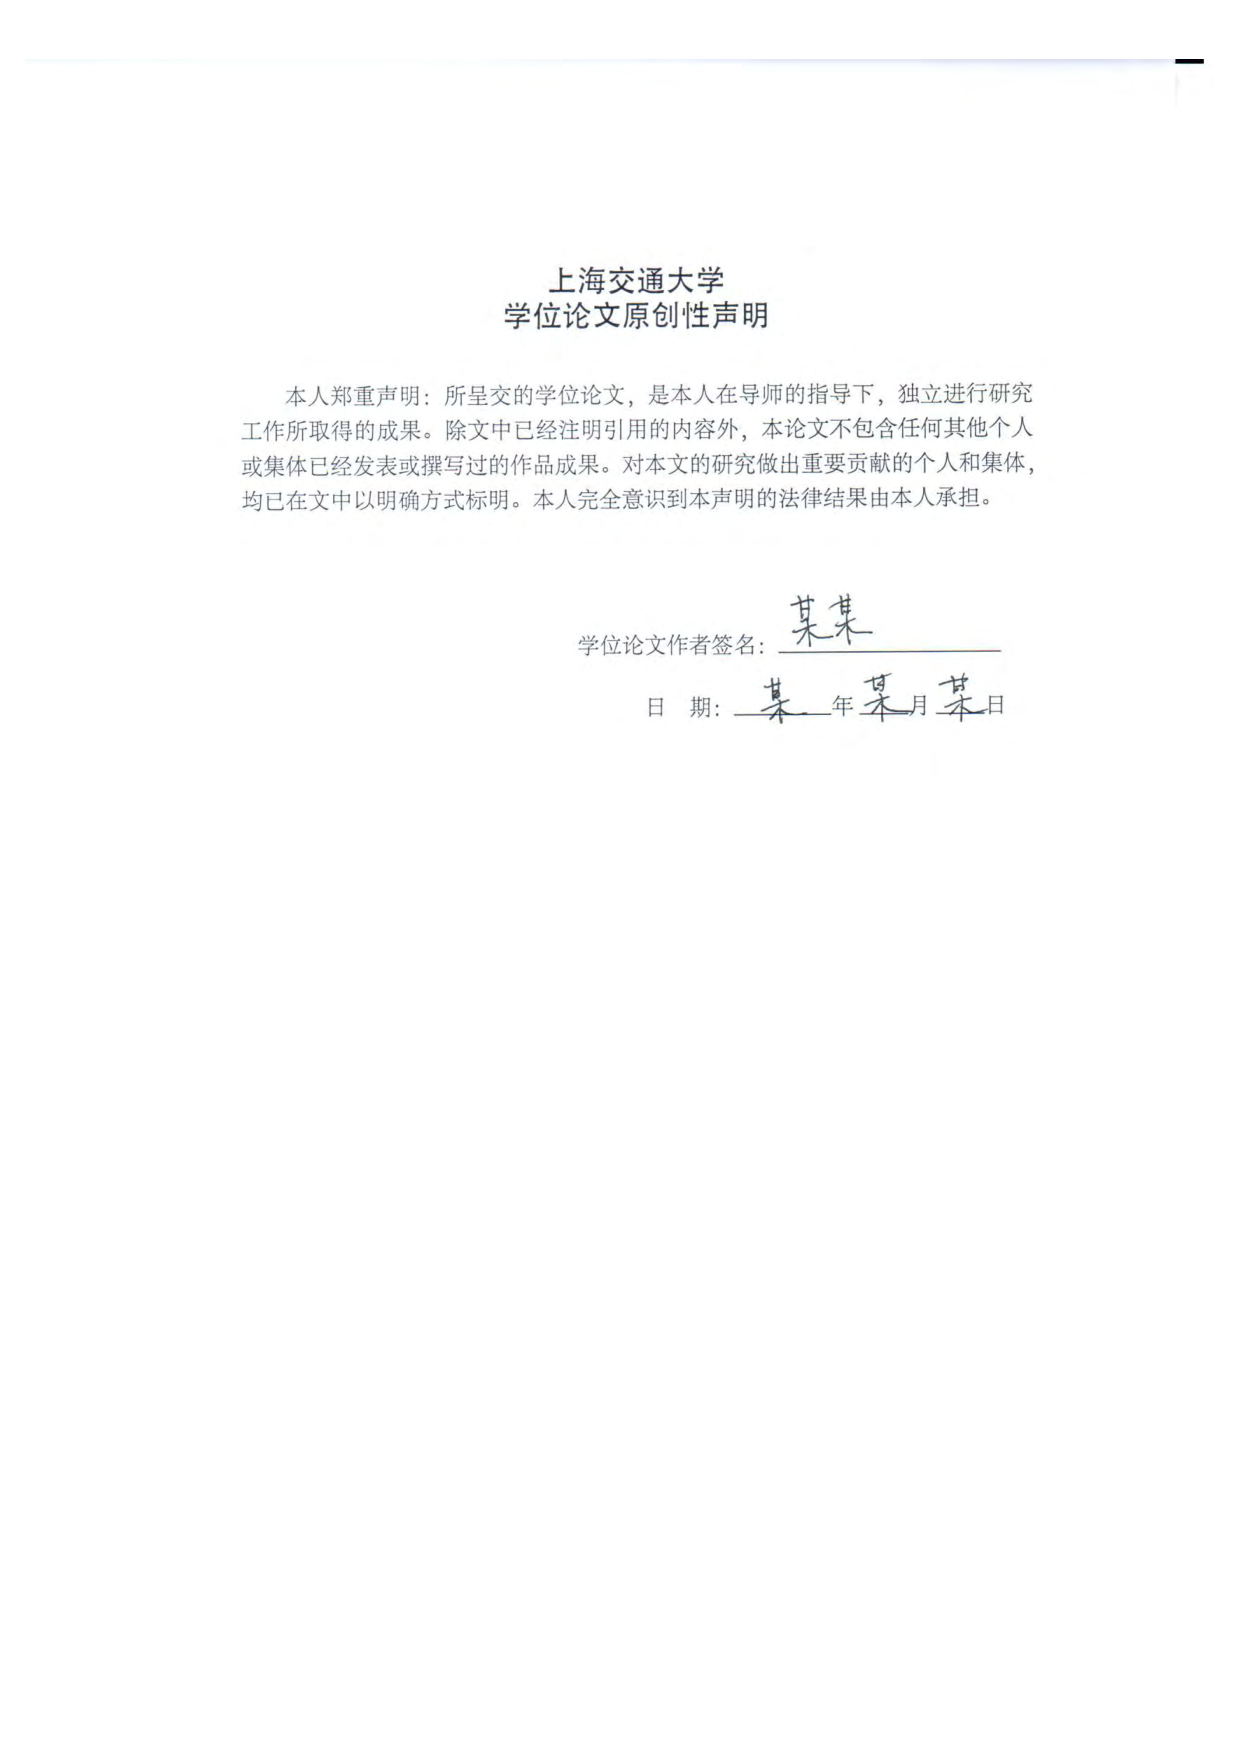
\includepdf{pdf/original.pdf}
	\cleardoublepage
	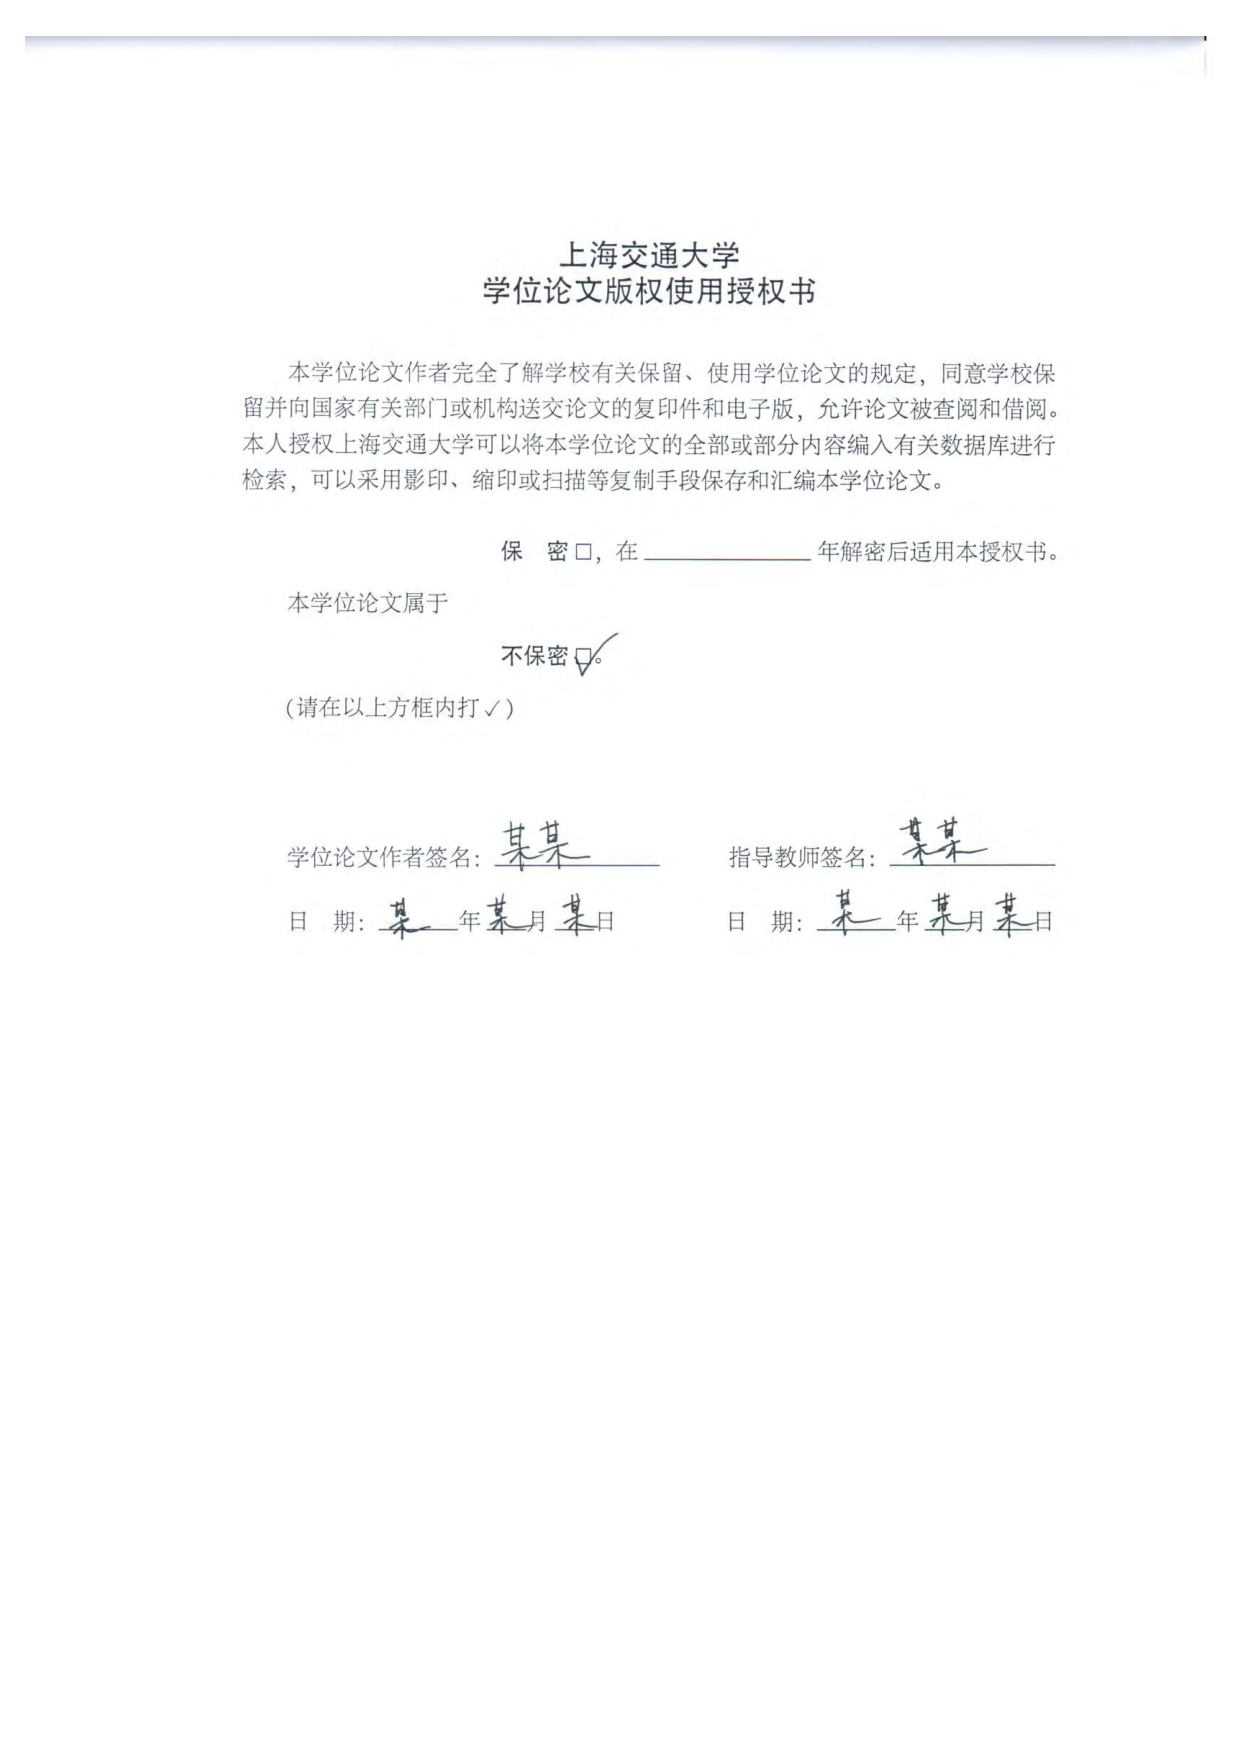
\includepdf{pdf/authorization.pdf}
	\cleardoublepage
\else
\ifsjtu@review\relax
% exclude the original claim and authorization
\else
	\makeDeclareOriginal
	\makeDeclareAuthorization
\fi
\fi
\makeatother


\frontmatter 	% 使用罗马数字对前言编号

%% 摘要
\pagestyle{main}
%# -*- coding: utf-8-unix -*-
%%==================================================
%% abstract.tex for SJTU Master Thesis
%%==================================================

\begin{abstract}

上海交通大学是我国历史最悠久的高等学府之一,是教育部直属、教育部与上海市共建的全国重点大学,是国家 “七五”、“八五”重点建设和“211工程”、“985工程”的首批建设高校。经过115年的不懈努力,上海交通大学已经成为一所“综合性、研究型、国际化”的国内一流、国际知名大学,并正在向世界一流大学稳步迈进。 

十九世纪末,甲午战败,民族危难。中国近代著名实业家、教育家盛宣怀和一批有识之士秉持“自强首在储才,储才必先兴学”的信念,于1896年在上海创办了交通大学的前身——南洋公学。建校伊始,学校即坚持“求实学,务实业”的宗旨,以培养“第一等人才”为教育目标,精勤进取,笃行不倦,在二十世纪二三十年代已成为国内著名的高等学府,被誉为“东方MIT”。抗战时期,广大师生历尽艰难,移转租界,内迁重庆,坚持办学,不少学生投笔从戎,浴血沙场。解放前夕,广大师生积极投身民主革命,学校被誉为“民主堡垒”。

新中国成立初期,为配合国家经济建设的需要,学校调整出相当一部分优势专业、师资设备,支持国内兄弟院校的发展。五十年代中期,学校又响应国家建设大西北的号召,根据国务院决定,部分迁往西安,分为交通大学上海部分和西安部分。1959年3月两部分同时被列为全国重点大学,7月经国务院批准分别独立建制,交通大学上海部分启用“上海交通大学”校名。历经西迁、两地办学、独立办学等变迁,为构建新中国的高等教育体系,促进社会主义建设做出了重要贡献。六七十年代,学校先后归属国防科工委和六机部领导,积极投身国防人才培养和国防科研,为“两弹一星”和国防现代化做出了巨大贡献。

改革开放以来,学校以“敢为天下先”的精神,大胆推进改革:率先组成教授代表团访问美国,率先实行校内管理体制改革,率先接受海外友人巨资捐赠等,有力地推动了学校的教学科研改革。1984年,邓小平同志亲切接见了学校领导和师生代表,对学校的各项改革给予了充分肯定。在国家和上海市的大力支持下,学校以“上水平、创一流”为目标,以学科建设为龙头,先后恢复和兴建了理科、管理学科、生命学科、法学和人文学科等。1999年,上海农学院并入;2005年,与上海第二医科大学强强合并。至此,学校完成了综合性大学的学科布局。近年来,通过国家“985工程”和“211工程”的建设,学校高层次人才日渐汇聚,科研实力快速提升,实现了向研究型大学的转变。与此同时,学校通过与美国密西根大学等世界一流大学的合作办学,实施国际化战略取得重要突破。1985年开始闵行校区建设,历经20多年,已基本建设成设施完善,环境优美的现代化大学校园,并已完成了办学重心向闵行校区的转移。学校现有徐汇、闵行、法华、七宝和重庆南路(卢湾)5个校区,总占地面积4840亩。通过一系列的改革和建设,学校的各项办学指标大幅度上升,实现了跨越式发展,整体实力显著增强,为建设世界一流大学奠定了坚实的基础。

交通大学始终把人才培养作为办学的根本任务。一百多年来,学校为国家和社会培养了20余万各类优秀人才,包括一批杰出的政治家、科学家、社会活动家、实业家、工程技术专家和医学专家,如江泽民、陆定一、丁关根、汪道涵、钱学森、吴文俊、徐光宪、张光斗、黄炎培、邵力子、李叔同、蔡锷、邹韬奋、陈敏章、王振义、陈竺等。在中国科学院、中国工程院院士中,有200余位交大校友;在国家23位“两弹一星”功臣中,有6位交大校友;在18位国家最高科学技术奖获得者中,有3位来自交大。交大创造了中国近现代发展史上的诸多“第一”:中国最早的内燃机、最早的电机、最早的中文打字机等;新中国第一艘万吨轮、第一艘核潜艇、第一艘气垫船、第一艘水翼艇、自主设计的第一代战斗机、第一枚运载火箭、第一颗人造卫星、第一例心脏二尖瓣分离术、第一例成功移植同种原位肝手术、第一例成功抢救大面积烧伤病人手术等,都凝聚着交大师生和校友的心血智慧。改革开放以来,一批年轻的校友已在世界各地、各行各业崭露头角。

截至2011年12月31日,学校共有24个学院/直属系(另有继续教育学院、技术学院和国际教育学院),19个直属单位,12家附属医院,全日制本科生16802人、研究生24495人(其中博士研究生5059人);有专任教师2979名,其中教授835名;中国科学院院士15名,中国工程院院士20名,中组部“千人计划”49名,“长江学者”95名,国家杰出青年基金获得者80名,国家重点基础研究发展计划(973计划)首席科学家24名,国家重大科学研究计划首席科学家9名,国家基金委创新研究群体6个,教育部创新团队17个。

学校现有本科专业68个,涵盖经济学、法学、文学、理学、工学、农学、医学、管理学和艺术等九个学科门类;拥有国家级教学及人才培养基地7个,国家级校外实践教育基地5个,国家级实验教学示范中心5个,上海市实验教学示范中心4个;有国家级教学团队8个,上海市教学团队15个;有国家级教学名师7人,上海市教学名师35人;有国家级精品课程46门,上海市精品课程117门;有国家级双语示范课程7门;2001、2005和2009年,作为第一完成单位,共获得国家级教学成果37项、上海市教学成果157项。

\keywords{\large 上海交大 \quad 饮水思源 \quad 爱国荣校}
\end{abstract}

\begin{englishabstract}

An imperial edict issued in 1896 by Emperor Guangxu, established Nanyang Public School in Shanghai. The normal school, school of foreign studies, middle school and a high school were established. Sheng Xuanhuai, the person responsible for proposing the idea to the emperor, became the first president and is regarded as the founder of the university.

During the 1930s, the university gained a reputation of nurturing top engineers. After the foundation of People's Republic, some faculties were transferred to other universities. A significant amount of its faculty were sent in 1956, by the national government, to Xi'an to help build up Xi'an Jiao Tong University in western China. Afterwards, the school was officially renamed Shanghai Jiao Tong University.

Since the reform and opening up policy in China, SJTU has taken the lead in management reform of institutions for higher education, regaining its vigor and vitality with an unprecedented momentum of growth. SJTU includes five beautiful campuses, Xuhui, Minhang, Luwan Qibao, and Fahua, taking up an area of about 3,225,833 m2. A number of disciplines have been advancing towards the top echelon internationally, and a batch of burgeoning branches of learning have taken an important position domestically.

Today SJTU has 31 schools (departments), 63 undergraduate programs, 250 masters-degree programs, 203 Ph.D. programs, 28 post-doctorate programs, and 11 state key laboratories and national engineering research centers.

SJTU boasts a large number of famous scientists and professors, including 35 academics of the Academy of Sciences and Academy of Engineering, 95 accredited professors and chair professors of the "Cheung Kong Scholars Program" and more than 2,000 professors and associate professors.

Its total enrollment of students amounts to 35,929, of which 1,564 are international students. There are 16,802 undergraduates, and 17,563 masters and Ph.D. candidates. After more than a century of operation, Jiao Tong University has inherited the old tradition of "high starting points, solid foundation, strict requirements and extensive practice." Students from SJTU have won top prizes in various competitions, including ACM International Collegiate Programming Contest, International Mathematical Contest in Modeling and Electronics Design Contests. Famous alumni include Jiang Zemin, Lu Dingyi, Ding Guangen, Wang Daohan, Qian Xuesen, Wu Wenjun, Zou Taofen, Mao Yisheng, Cai Er, Huang Yanpei, Shao Lizi, Wang An and many more. More than 200 of the academics of the Chinese Academy of Sciences and Chinese Academy of Engineering are alumni of Jiao Tong University.

\englishkeywords{\large SJTU, master thesis, XeTeX/LaTeX template}
\end{englishabstract}



%% 目录、插图目录、表格目录
\tableofcontents
\listoffigures
\addcontentsline{toc}{chapter}{\listfigurename} %将插图目录加入全文目录
\listoftables
\addcontentsline{toc}{chapter}{\listtablename}  %将表格目录加入全文目录
\listofalgorithms
\addcontentsline{toc}{chapter}{算法索引}        %将算法目录加入全文目录

%# -*- coding: utf-8-unix -*-
\chapter{主要符号对照表}
\label{chap:symb}

\begin{longtable}{cl}
$\phi$ & 浮空器的滚转角 \\
$\theta$ & 浮空器的俯仰角 \\
$\psi$ & 浮空器的偏航角 \\
$u$ & 机体坐标系下的$x$方向线速度 \\
$v$ & 机体坐标系下的$y$方向线速度 \\
$w$ & 机体坐标系下的$z$方向线速度 \\
$p$ & 机体坐标系下绕$x$轴的转动角速度 \\
$q$ & 机体坐标系下绕$y$轴的转动角速度 \\
$r$ & 机体坐标系下绕$z$轴的转动角速度 \\
$\mathbf{M}\in\mathbb{R}^{6\times6}$ & 浮空器的惯性矩阵\\ 
$x_G,y_G,z_G$ & 浮空器的重心位置 \\
$x_B,y_B,z_B$ & 浮空器的浮力中心位置 \\
$m$ & 浮空器的总质量 \\
$m_{11},\cdots,m_{66}$ & 浮空器的附加质量 \\
$I_x,I_y,I_z$ & 浮空器绕$x,y,z$轴的转动惯量 \\
$\mathbf{F_{gb}}\in\mathbb{R}^{6\times1}$ & 浮空器重力与浮力的合力 \\
$\mathbf{F_a}\in\mathbb{R}^{6\times1}$ & 浮空器所受气动力 \\
$\mathbf{F_i}\in\mathbb{R}^{6\times1}$ & 浮空器所受科氏力 \\
$\mathbf{F_t}\in\mathbb{R}^{6\times1}$ & 浮空器的总控制输入 \\
$f_x$ & 浮空器所受$x$方向推力输入 \\
$f_y$ & 浮空器所受$y$方向推力输入 \\
$f_z$ & 浮空器所受$z$方向推力输入 \\
$m_x$ & 浮空器所受绕$x$轴方向力矩输入 \\
$m_y$ & 浮空器所受绕$y$轴方向力矩输入 \\
$m_z$ & 浮空器所受绕$z$轴方向力矩输入 \\
$B$ & 浮空器所受浮力 \\
$G$ & 浮空器所受重力 \\
$q_{\infty}=\frac{1}{2}\rho v_{wind}^2$ & 浮空器所受气动压强 \\
$\mathrm{Vol}$ & 浮空器的体积 \\
$S_{ref}=\mathrm{Vol}^{2/3}$ & 浮空器的气动参考面积 \\
$L_{ref}=\mathrm{Vol}^{1/3}$ & 浮空器的气动参考长度 \\
$\Omega$  & 浮空器$x$轴与空气流速方向的迎角 \\
$C_x$ & 浮空器的水平气动系数 \\
$C_z$ & 浮空器的纵向气动系数 \\
$C_{my}$ & 浮空器的俯仰力矩气动系数 \\
$R_p$ & 浮空器的螺旋桨到其体积中心的距离 \\
$\mathbf{J_1}$ & 机体系到地面坐标系的线速度转换矩阵 \\
$\mathbf{J_2}$ & 机体系到地面坐标系的角速度转换矩阵 \\
$\rho$ & 飞行高度下的空气密度 \\
$\mathbf{S}$ & 气动矩阵 \\
\end{longtable}
 % 主要符号、缩略词对照表

\mainmatter	% 使用阿拉伯数字对正文编号

%% 正文内容
\pagestyle{main}
%# -*- coding: utf-8-unix -*-
%%==================================================
%% chapter01.tex for SJTU Master Thesis
%%==================================================

%\bibliographystyle{sjtu2}%[此处用于每章都生产参考文献]
\chapter{绪论}
\label{chap:introduction}

\section{研究背景和意义}
飞行器的发明至今已有100多年的历史。人类已经发展出了适应于不同飞行高度和任务的多种飞行器。在20km高度以下,通常以固定翼飞机、直升飞机和中低空飞艇为主;在高度100km以上,通常以卫星为主;而在20km-100km的高度通常以平流层飞艇为主。飞行器按照功能又可分为载人飞行器和无人飞行器:载人飞行器在民航运输、太空探测领域的应用前景宽广;而无人飞行器在抢险救灾、卫星通信等领域有巨大的潜力。在军事方面,飞行器还可用于敌情侦查,危险区域探测、执行无人任务、充当通信中继平台等方面。

但是,自从飞行器发明以来,系统故障就是一个不可避免的话题。由于系统长时间运行、材料设备老化、系统过于复杂甚至飞行员操作失误等多种原因,任何飞行器都会在运行过程中发生故障。尤其是飞行器被大量用于民航领域之后,空难代价十分巨大。 历史上单单因飞机引擎熄火引起的空难事故就有很多。2015年6月30日,印尼军用大力士运输机发生空难\footnote{\url{https://www.kinitv.com/video/20264O102}}。军机在引擎熄火后试图折返,不过最终却失控撞向附近的大楼和住房。事故后发生后,调查队伍发现军机的其中一个引擎突然熄火,相信是造成军机坠毁的主要原因。2015年2月4日,台湾复兴航空一家GE235-ATR72型班级从台北松山机场起飞后不久,坠毁在机场10跑道末端东南东方约5.4公里处的基隆河,机上共58人,包括驾驶舱内3名机师在内,有43人罹难\footnote{\url{http://www.scio.gov.cn/zhzc/8/3/document/1439904/1439904.htm}}。据调查引擎熄火也是空难发生的主要原因。1982年6月24日,英国航空一班原定由伦敦希思罗机场飞往纽西兰奥克兰国际机场,中途停孟买、清奈、吉隆坡、柏斯及墨尔本的班机。当日,航班由一架注册编号G-BDXH的波音747-200飞行。这架班机在印尼附近的空域飞入一片火山灰云,导致四具引擎全部熄火,所幸最终平安降落在雅加达哈利姆·珀达纳库苏马国际机场。此外还有很多如加拿大航空143号班机事故\footnote{https://baike.baidu.com/item/加拿大航空143号航班事故/7365085?fr=aladdin}和伊朗班机事故\footnote{\url{http://newspaper.jfdaily.com/jfrb/html/2014-08/11/content_2560.htm}}。这些事故的共性都是执行机构(引擎)发生了故障,从而直接导致了飞行器的危险。虽然经验丰富的飞行员可以减小这类事故的伤害,但是大多数情况下,执行机构失效还是会对飞行器的乘客安全造成极大的威胁。

容错控制不仅仅只对于载人飞行器有重要意义。对于无人自主飞行器而言,没有了飞行员的干预,其自主性大大提高,飞行器性能和工作时长都有了明显提高。但随之带来的就是更高的控制算法要求。比如飞行器要有鲁棒的控制方案以应对各种各样的执行机构失效问题;飞行器需要在强干扰的情况下维持稳定姿态并在有可能的条件下继续完成给定任务。这些需求都是迫切和重要的,因此,在提高飞行器的自主性、减少人为干预的同时,必须提出有效的容错控制方案。否则,无人自主飞行器的实现必将遇到极大的困难。

而轻于空气的浮空器(Lighter-than-air, LTA)作为飞行器中人们研究最少的一类,应用前景十分广泛。浮空器分为自主浮空器与系留浮空器。系留浮空器通常高度限制在1000m以下,不需要过多控制,但由于受风影响较大,且高度有局限性,应用前景比较窄。而自主浮空器则具有高度灵活可变,飞行距离长的特点,不受系留的限制,因而应用前景更为广泛。自主浮空器,尤其平流层浮空器的设计非常复杂,由于平流层浮空器通常需要具有很长的飞行时间,并工作在极端恶劣的自然环境中,因此其执行机构不可避免地会发生故障。如果不加以对应的容错控制算法,自主浮空器就不能很好地完成其自主任务。

浮空器的研究曾在20世纪初非常流行。当时人们以氢气作为填充气体。后来因为德国“兴登堡”号飞艇的事故\footnote{\url{https://en.wikipedia.org/wiki/Hindenburg_disaster}},人们停止了对飞艇的研究。但是在20世纪末期到21世纪初,由于材料科学的发展和氦气的广泛使用,浮空器的飞行性能和安全性都得到了大大提高,同时由于卫星和飞机的发展,临近空间的军事价值迅速提升,因此针对平流层浮空器的研究重回人们的视野\cite{lutz1998drag,gomes1998airship,jose2002influence,Bessert2005731}。

事实上,由于设计、制造浮空器耗费资金巨大,其安全运行一直被工程师和科学家们重视。在上世纪90年代以前,人们已经熟知通过设计冗余的执行机构,进行对多输入多输出(MIMO)的系统的反馈控制器设计\cite{makarand1988actuator,conner1979fail}。但是控制器的表现都不太理想。甚至是明知在控制器故障之后,剩余控制器有足够能力保持系统稳定的前提下,控制系统仍然无法让被控对象保持稳定\cite{119629}。因此,设计一个能够容忍执行机构或传感器故障,并保持系统闭环行为的控制系统,在20世纪80年代的时候开始成为学术研究的热点。

浮空器的容错控制意义非常深远。无论商用还是军用浮空器,都搭载了十分复杂的控制系统。由于系统的复杂性,许多零部件不可避免地会发生不可预知的错误;而不同系统之间的互相依赖、不同变量之间的耦合都会将任何一个小故障放大,甚至影响飞行安全。因此,针对浮空器的容错控制的研究意义十分重大。

\section{研究现状与存在问题}
浮空器的容错控制与飞行器的容错控制关系紧密。由于浮空器的动力学模型与一般飞行器大体相同,所以很多用于一般飞行器的算法也可以在浮空器上使用。因此,本节主要阐述的是一般飞行器的容错控制的分类、方法和效果。并结合浮空器本身的特性,阐述浮空器容错控制的特异性和难点。

飞行器的容错控制是非线性系统容错控制的一个分支,非线性系统的容错在国内外也已经有很多研究成果。浮空器的容错控制研究,没有跳出非线性系统的范畴,研究方法也与非线性系统类似。现在学术界对容错控制的分类方法有一些不同的观点。Blanke等\cite{BLANKE1997693}从工程角度把容错控制系统分成三层——底层(控制层)、中层(探测与重构)和高层(监测)。许域菲\cite{xuyufei2011}对比了增益预置(Gain Scheduling)、特征结构配置(Eigenvector Assignment)、自适应控制(Adaptive control)、滑模变结构控制(Sliding mode control)、反演思想(Backstepping)和智能控制(Intelligence control)这六种先进容错控制方法的优缺点。Yin在做航天器姿态容错控制的工作中,认为将容错控制分为故障检测与控制器重构\cite{7407616}。尽管这些分类方法从不同角度阐述了容错控制的研究现状,但是目前最主流的分类是将容错控制根据设计思路不同分为被动容错控制和主动容错控制\cite{Zhang2008229,5160615,jiang2005fault,gaozhifeng2011,xuyufei2011,wangdejun2014},文献\citen{Jiang201260}阐述了被动容错与主动容错的本质上的不同,本文也采纳这一分类观点。而其中主动容错控制又可分为故障检测与诊断和容错控制器设计两个步骤,目前这两个步骤也各自都是相关领域的研究热点。在具体的控制器设计方法上,被动容错控制和主动容错控制有很多相似之处。本节中,\newref{subsec:passive} 主要介绍非线性系统的被动容错研究;\newref{subsec:fdd} 主要介绍故障检测与诊断的研究成果;\newref{subsec:active} 主要介绍非线性系统的主动容错控制研究成果。

\subsection{被动容错控制}\label{subsec:passive}
被动容错控制(Passive Fault-tolerant Control, PFTC),其思想是针对一种或几种错误,使用鲁棒控制的一些技巧,构造一个控制器,使得这几种已知错误发生时对控制器的影响减到最小或忽略不计\cite{jiang2005fault,6859271}。在PFTC中,“被动”表示控制器一旦构造好就不再改变事先设计好的参数和结构,当系统发生任何被考虑在内的故障时,这个控制器能自动对故障进行补偿,保证系统的闭环动态品质在一个可接受的范围内。其优点是运算速度快、无需掌握错误的在线信息,一切运算都在离线时算好,控制器实施起来较为简单;缺点是必须事先想好错误发生的种类和影响,并将其表现在系统模型的参数变化中,只能应对已知的几种错误,无法应对不可预知类型的错误。同时,由于被动容错需要用一种控制器应对多种错误,那么这种控制器势必要设计得非常保守,因而很难达到最优控制效果\cite{jiang2005fault}。

为了直观地说明被动容错控制的思想,在此引用文献\citen{Jiang201260}中的一张示意图——图\newref{fig:asp}表示了不同错误下的一个控制器空间示意图。其中三个大圆表示三种错误下,能够保持系统的可接受的控制器范围。每种错误都有一个对应的最优控制器解(图中Optimal solution)。我们如果要设计一种被动容错控制器,同时处理这三种错误,那么只能将控制器设计在图中三圆的公共区域(图中阴影区域)。显然,这对三种错误来说各自都不是最优解,可以说需要处理的错误种类越多,系统的相应距离最优解越遥远。特别是图\newref{fig:aspoverlap}所示的几种情况,三个圆没有交集,那么理论上针对这样系统的被动容错控制是不存在的,这时只能对错误进行取舍。
\begin{figure}[!htp]
    \centering
    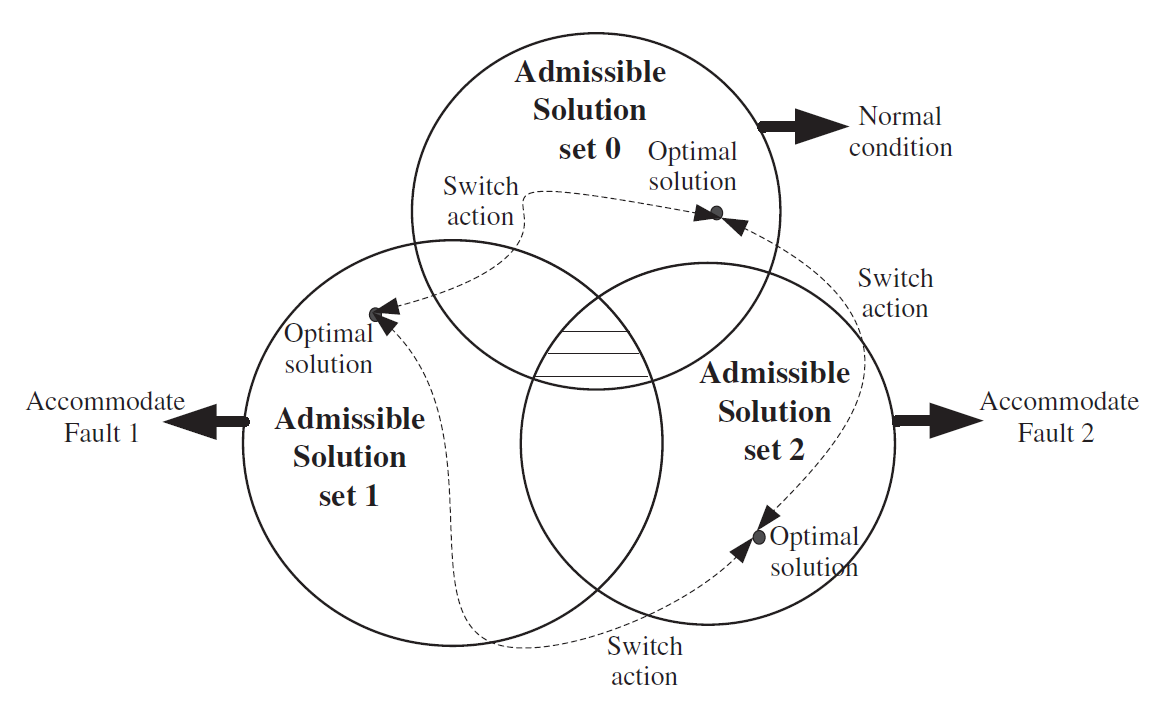
\includegraphics[width = 0.9\textwidth]{figure/admissiblesp.png}
    \bicaption[fig:asp]{可接受的控制空间示意}{可接受的控制空间示意\cite{Jiang201260}}{Fig.}{The acceptable space}
\end{figure}
\begin{figure}[!htp]
    \centering
    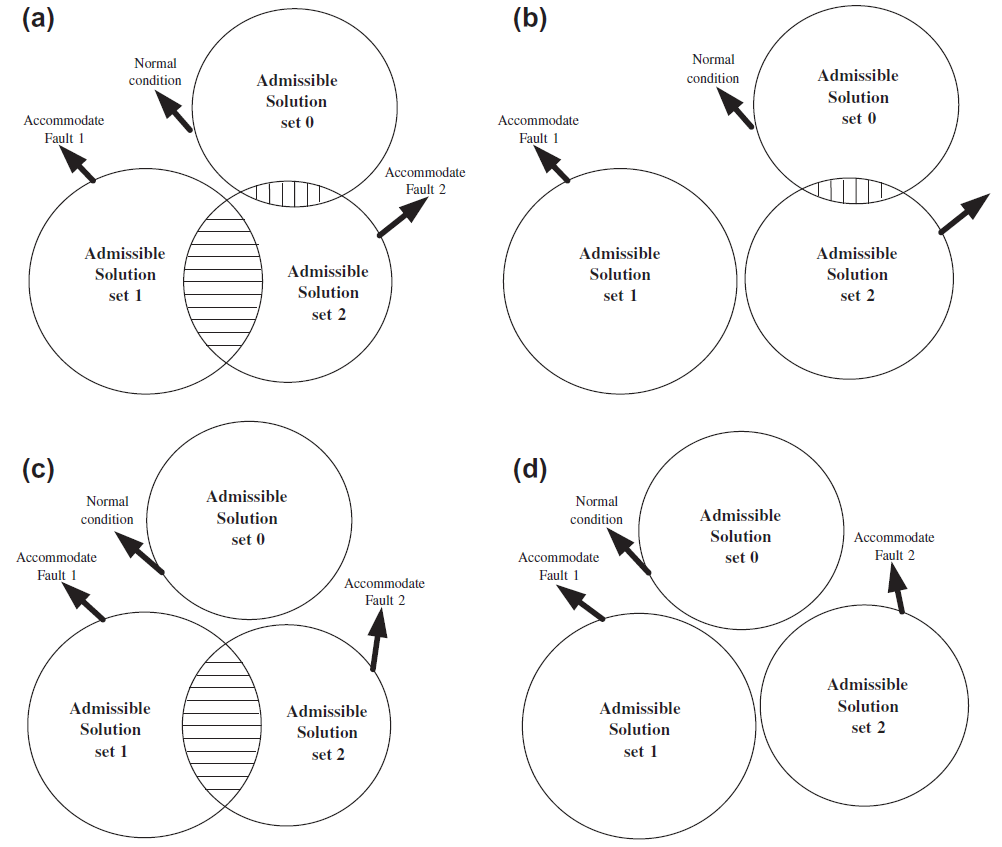
\includegraphics[width = 0.9\textwidth]{figure/aspoverlap.png}
    \bicaption[fig:aspoverlap]{其他控制器空间示意}{其他控制器空间示意\cite{Jiang201260}}{Fig.}{Other controller's space}
\end{figure}

被动容错控制文献中被称为可靠控制(Reliable control)。“可靠”的概念第一次由Siljak于1980年提出\cite{siljak1980},经过Date和Cho等人的发展\cite{70346,4790503},最终在1992年由Robert J. Veillette进行系统地总结\cite{119629},提出了“可靠控制”这一概念。往后,文献中的凡是以被动容错控制思路设计的控制器,都以reliable control呈现。

被动容错控制的设计方法有很多种,在$H_\infty$优化\cite{119629,7850999}、LMI方法\cite{7795198,974340,1236798}、LQ方法\cite{VEILLETTE1995137,847106,866928},滑模控制方法\cite{4160860},模糊系统\cite{7795198,7505963,Zha20173267},动态预补偿结合特征结构配置\cite{Jiang2000Design,ZHAO19981267},去中心化观测器\cite{70346}等方面均有相关研究成果。其中文献\cite{ZHAO19981267}首次给控制器冗余和错误构建了数学模型。另外,根据针对系统错误的不同,被动容错控制还可以分为针对执行机构失效\cite{ZHAO19981267,974340,VEILLETTE1995137,1236798,Tian20101907,Li20132455,7353144,7863042,70346,866928}、时变错误\cite{7850999,CHEN2004349,6064886}和随机错误\cite{7795198,7505963,5540530,Zha20173267}。基于控制器重构的被动容错控制也受到了不少关注\cite{6859271},这一类控制器通过重新分配控制量的方法来使控制器适应多种错误。
国内外也有不少文献对被动容错控制提出了分类方法。国外文献中,Fekih\cite{6859271}用鲁棒控制的分类方法把被动容错控制分为了数量反馈理论法、$H_\infty$范数优化法\cite{4079591}、LQ控制法\cite{Staroswiecki20072070}、$\mu$同步法和变结构方法。国内文献中,王德军\cite{wangdejun2014}、许德智\cite{xudezhi2013}和高志峰\cite{gaozhifeng2011}都将被动容错控制分为可靠镇定、完整性与联立镇定三类方法。肖冰\cite{xiaobing2014}认为在航天器姿态控制中,被动容错控制可以与主动容错控制的控制器重构部分做为一个方向共同研究。他将航天器姿态容错控制方法,分为基于自适应技术(Adaptive)的方法、基于滑模控制的方法和基于控制分配的方法三类,这一点在Yin. S的论文中\cite{7407616}也得到了有力的支撑。

\subsection{故障检测与故障诊断}\label{subsec:fdd}

故障检测(Fault Detection)与故障诊断(Fault Diagnosis)是两个不同的概念。故障检测,一般指系统对是否发生故障进行在线检测;而故障诊断,指的是在检测到故障的基础上,判断故障的类型和严重性。故障检测与诊断是主动容错控制器设计前的必经步骤。目前已经有很多综述文章阐述了故障检测与诊断的研究现状\cite{Venkatasubramanian2003293,6859271,Zhang2008229,7407616,6423903,Marzat2012modelbased,Jiang201260,5282515,Venkatasubramanian2003293,Venkatasubramanian2003A}。其中具体对故障检测的分类也有一些不同。

Inseok Hwang\cite{5282515}在文献中将故障检测分为硬件冗余(Hardware Redundancy)和分析冗余(Analytical Redundancy)两类。而其中硬件冗余主要是设计多传感器来尽可能明确地检测故障,可分为交叉频道监控(Cross channel monitoring, CCM)、残差生成(Residual Generation)和信号处理(Signal Processing)方法;分析冗余主要是用数学模型直接对系统当前状况进行估计,不需要多余的硬件,因此也更高效,分析冗余又可分为定性(Qualitative)方法和定量(Quantitative)方法。 Fekih\cite{6859271}和Hwang\cite{5282515}都认为所有故障检测都由三个步骤构成:残差生成(Residual Generation)、残差评估(Residual Evaluation)和最终判断(Decision Making)。在此基础上,诊断方法可以分为基于模型(Model-Based)的方法和不基于模型(Model-Free)的方法。其中基于模型的方法有模糊、神经网络、专家系统等方法\cite{Patan2008Artificial},不基于模型的方法主要是基于算法和统计的手段。而残差评估则可以分为序列概率检验(Sequential probability ratio test)和通用比例检验(Generalized Likelihood Ratio Test)等统计学上的方法\cite{5282515}。此外,Yin的文献\citen{7407616}中把故障检测分为两大类——基于模型的方法和基于数据的方法。其中基于模型的方法依赖于系统模型,而当模型不准确时,可以使用纯数据方法。

本文的观点与Fekih\cite{6859271}和Hwang\cite{5282515}各有相似之处,认为不论基于模型还是数据,故障检测的思路都是通过设计一个残差函数来对故障进行判断,具体在残差函数的设计思路及依赖上,才有了基于模型、不基于模型或是基于数据的区别。因此,本文故障检测的步骤分为残差生成、残差评估两个步骤。而残差生成作为故障检测的核心部分,又可以分为基于模型的方法和基于数据的方法。
\subsubsection{基于模型的方法}
对于基于模型的方法,文献\citen{Marzat2012modelbased}做了很好的综述。Venkatasubramanian的两篇综述\citen{Venkatasubramanian2003293,Venkatasubramanian2003A}将基于模型的故障检测分为定性方法和定量方法。通常来说,该类故障检测分为残差生成、残差评估两个环节\cite{Marzat2012modelbased},系统框图如图\newref{fig:FDDProcess}所示。在残差生成环节,使用系统的执行器输入和传感器数据来预测系统接下来的行为;然后将预测行为与系统实际行为进行比较。这里介绍几种基于模型的方法,分别是参数估计类方法、状态估计类方法、奇偶校验空间方法、去耦合类方法和闭环方法。
\begin{figure}[htp]
    \centering
    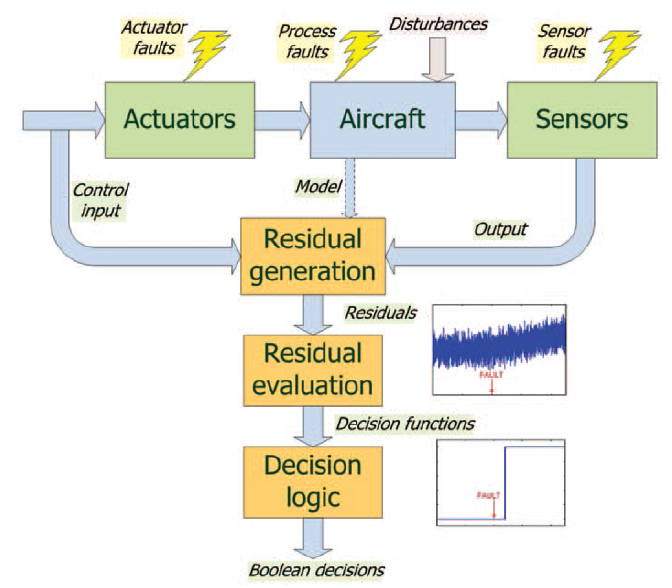
\includegraphics[width = 0.9\textwidth]{FDDProcess.png}
    \bicaption[fig:FDDProcess]{一种典型的故障检测机制}{一种典型的故障检测机制}{Fig.}{A typical fault detection scheme}
\end{figure}

\paragraph*{参数估计类方法}由于系统方程中的参数很可能没有直接的物理意义,而有些能测量到的物理量又不能明显地给出系统是否有错误的判断,参数估计故障诊断方法就是在这种背景下产生的。这类方法的思路是:把系统方程中的参数$\theta$与系统中具有实际物理意义但不能测量到的变量$p_a$(如舵偏角等)建立方程
$$\theta = g_p(p_a)$$
然后首先依据系统观测方程
$$y=h(u,\theta)$$
测量到的$y$对参数$\theta$进行估计,得到$\hat{\theta}$;再通过$p_{a0} = g_p^{-1}(\hat{\theta})$求出可能的$p_{a0}$。最后将得到的$p_{a0}$输入事先设计好的残差函数,与事先设置好的可接受的$p_a$值进行比较。这是一种比较经典的方法,文献多在2000年以前出现\cite{ISERMANN1984387,FRANK1990459,ISERMANN1993815,411478,BLOCH19951709},其中对参数$\hat{\theta}$的辨识也成为了新的研究方向\cite{ISERMANN1993815,411478,BLOCH19951709},涉及到的方法多为最小二乘、卡尔曼滤波等一些最优估计的方法。参数估计的计算强度较大是这类方法的缺点,文献\cite{Villemonteix2009Bayesian}对参数估计提出了一种贝叶斯(Bayesian)优化方法。在残差函数的设计中,也可以设置多个可接受的$p_a$值的集合,详见文献\citen{Kieffer2011Guaranteed,Puig2010Fault}。

\paragraph*{状态估计类方法}状态估计类方法的思路是通过对系统状态的估计与传感器测量的数据做对比,得到系统是否发生错误的判决。通常可以根据对不确定性的处理分为确定性方法、随机方法和有界误差方法\cite{Marzat2012modelbased}。

确定性方法\cite{1098323,ALCORTAGARCIA1997663}不考虑系统的误差和扰动,直接在模型中推导观测误差与错误的关系。Luenberger观测器\cite{1098323}是这种方法第一次被应用到线性系统上。由于非线性系统线性化的时候会产生误差,因此又有了处理非线性系统的扩展Luenberger观测器(Extended
Luenberger Observer, ELO)\cite{Nejjari2008Extended,ZEITZ1987149}。此外,由于非线性系统的复杂性,也有很多种观测器得到了研究,如自适应观测器(Adaptive observers)\cite{878691,Zhang2010290}、高增益观测器(High-gain observers)\cite{Busvelle2002HIGH}、滑模观测器(Sliding Mode Observers)\cite{Edwards2011Sliding,1269645}和基于偏微分方程(partial-differential equation)设计的新型观测器\cite{5717995}。

随机方法中,通常假定系统的噪声扰动服从高斯分布(Gaussian Distribution),在处理线性系统时以卡尔曼滤波器(Kalman Filter)为代表。基于卡尔曼滤波器的容错方法首先在文献\cite{MEHRA1971637}中提到,而后\cite{NIKOUKHAH19941851,539440,willsky1986detection}做了后续延伸工作。处理非线性系统时,有扩展卡尔曼滤波(Extended Kalman Filter, EKF)、无迹卡尔曼滤波(Unscented Kalman Filter, UKF)和粒子滤波(Particle Filter, PF)。扩展卡尔曼滤波通过对非线性系统线性化来使用卡尔曼滤波\cite{CHANG19952861};无迹卡尔曼滤波则不对系统线性化,通过一些系统状态采样点来逼近系统状态的高斯分布\cite{4252507,XIONG2005113}。粒子滤波则可适用于非线性非高斯分布的噪声,它采用蒙特卡洛方法对错误进行建模并估计\cite{1271398,971661}。

有界误差方法不同与上面两种。上面两种都使用了显示的故障模型或概率分布,而有界误差方法使用故障的上界进行处理。这类方法的文献如区间分析法\cite{4547434}和神经-模糊方法\cite{Korbicz2007609}。

\paragraph*{奇偶校验空间法}奇偶空间校验(Parity Space)方法比较容易从直观上理解,是一种解除系统状态和错误之间的耦合,从而方便设计出只跟故障有关的残差函数\cite{patton1991review,GERTLER1995627}的方法。具体来说,对于一个静态线性观测系统:
\begin{equation*}
    \mathbf{y} = \mathbf{Cx} + \mathbf{E_fw_f}
\end{equation*}
其中$\mathbf{w_f}$是系统错误,$\mathbf{y}$是观测变量。此时如果设计一个矩阵$\mathbf{W}$,使得$\mathbf{WC=0}$,那么残差函数$\mathbf{Wy}$就只与系统错误$\mathbf{w_f}$有关了,可以依次设计残差函数。对于动态系统,可以用\citen{Marzat2012modelbased}中提及的方法先把系统化成静态系统的形式。对于非线性系统,则可以用线性化、仿射变换等方式来处理,详见文献\citen{Staroswiecki2001687,shumsky2007redundancy,1024022,948476}。

\paragraph*{去耦合类方法}在故障检测设计残差函数时,经常遇到的一个问题是如何区分系统的正常扰动和意外故障。一个理想的残差函数应该满足\cite{1104419}:1)只对系统错误有响应,对系统状态和扰动无响应;2)在系统没有故障的时候,能够随着时间的推移收敛到0。这里介绍四种去耦合类的方法。

第一种是特征结构分配(Eigenstructure Assignment)的方法\cite{261546}。该方法给系统的输出估计偏差$\mathbf{e_y}$左乘了一个权值矩阵$\mathbf{W}$作为残差函数\cite{261546,RNC:RNC523}。同样的方法也可以用在奇偶校验空间的残差设计中,使得残差对系统扰动不敏感\cite{doi:10.1080/00207179508921908}。

第二种是未知输入观测器(Unknown-Input Observer, UIO)。这种观测器能够在估计系统状态的同时将外部扰动的影响降到最小\cite{jie1996design,1657536,220921}。简单将未知输入观测器的原理说明如下,假设系统如\neweqref{eq:UIO1}所示。
\begin{equation}\label{eq:UIO1}
\begin{cases}
\dot{x} = Ax+Bu+E_dw_d+E_fw_f \\
y = Cx 
\end{cases}
\end{equation}
其中$w_d$代表扰动,$w_f$代表错误。针对该系统的位置输入观测器设计如\neweqref{eq:UIO2}所示
\begin{equation}\label{eq:UIO2}
\begin{cases}
\dot{\hat{x}}=F\hat{x}+TBu+(K_1+K_2)y \\
\mathbf{r} = (I-CH)y-C\hat{x}
\end{cases}
\end{equation}
其中,$\mathbf{r}$为残差函数,$F,T,K_1,K_2,H$都是设计参数,需满足以下条件:
\begin{equation*}
\begin{cases}
(HC-I)E_d=0\\
T = I - HC\\
F= I-HCA-K_1C\\
K_2=FH
\end{cases}
\end{equation*}
只要这样的观测器存在,那么可以用\citen{4101989}中提及的DOS(Dedicated observer scheme)或者GOS(General observer scheme)的方法进行故障检测系统设计。

第三类方法是$H_{\infty}$方法,这种策略适合精确解耦无法达到的情况\cite{doi:10.1080/002071799220704,Henry2005251}。$H_{\infty}$方法的思想是,根据$H_{\infty}$范数设计残差函数,使得错误对其影响最大,并且扰动对其影响最小。运用线性矩阵不等式(Linear Matrix Inequality, LMI)是解决这类问题的标准化方法\cite{Zhong2003543}。

第四类是非线性几何方法。微分几何的方法\cite{928586,Bokor2009113}能够检测是否存在一个只对一种错误敏感的滤波器\cite{Marzat2012modelbased}。微分代数的方法也有文献,如\citen{berdjag:hal-00198435}。此外,还有一种逆向的方法\cite{edelmayer2004input,doi:10.1080/00207170802582215,1102181}。该种方法不同于大多数故障检测方法。大多数故障检测系统都使用估计系统输出与测量到的系统输出作比较或设计残差函数,这种逆向方法使用系统输入与前一时段发送给系统执行器的输入作比较。由于大多数飞行器都装备了惯性测量元件(Inertia Measurement Unit, IMU),针对利用惯性测量元件的故障检测也有相关文献,如\citen{MARZAT2010951,5676073}。

\paragraph*{闭环方法}前面介绍的几种故障检测方法都是未考虑反馈控制的开环检测方法。但事实上控制信息能极大地辅助故障检测。比如设计一个辅助控制器添加到系统本身的输入中\cite{NIEMANN2006587,ASHARI2009192}。文献\citen{ASHARI2009192,4602147}将这种方法应用到无人机上,通过添加一个微小的正弦控制量的方法进行故障检测。但是这种方法需要非常小心,需要保证添加的控制量不会严重干扰系统的稳定性和表现\cite{Niemann2006Active}。

鉴于以上原因,闭环方法需要在控制表现和故障检测能力中做取舍。Jacobson\cite{92987}设计了同时能够控制和故障检测的模型。 相关的多目标优化问题也成为了研究的热点。Henry\cite{Henry2005251}提出了一种对这类问题的建模,并用线性矩阵不等式得到了问题的最优解。Niemann\cite{649678}对闭环故障检测方法的效果与开环方法做了对比。

\subsubsection{基于数据的方法}\label{subsubsec:databased}
当系统模型十分不精确,没有显示表达甚至无法获取的时候,人们对系统的认知途径只能通过测量的方式。通过测量到的数据,加上一定的分析方法,能够最大限度地还原系统的面貌。这时,系统相当于一个黑盒,其历史运行数据是掌握其运行规律的唯一方法。通过数据,不仅可以对系统进行故障诊断,还能进行控制器设计。这一类方法统称基于数据的方法。在1991年,Jackson已经使用多变量统计学进行故障检测。

Yin在基于数据的方法有较多的研究文献\cite{6717991,7394158,7067026,6748057,7297846,7407616}。其中文献\cite{6717991,6748057,7407616}提供了基于数据的故障诊断的文献综述。此外,Qin\cite{Qin2012220}、Marzat\cite{Marzat2012modelbased}、Venkatasubramanian\cite{Venkatasubramanian2003327}都做了对基于数据故障检测方法的综述。其中Qin\cite{Qin2012220}对残差生成、残差判别、故障识别等多个步骤都做了综述。由于残差生成是故障检测的核心步骤,这里介绍几种基于数据的残差生成的方法。几种方法的思路都是给系统的正常状态建模,或者建立一个系统正常状态下的向量空间。如果测量得到的数据偏离了这个空间,那么就说明系统出现了错误。学术界这一类容错的方法有专家系统(Expert System)方法、主成分分析法(Principle Component Analysis, PCA)和模式识别方法等。由于专家系统方法现在应用较少,下面主要介绍主成分分析法和模式识别方法。

\paragraph*{主成分分析法}
主成分分析\cite{jolliffe2002principal}在工程中有非常广泛的应用,适用于能获取到大量历史运行数据的系统。Ding\cite{Ding2010138}对标准主成分分析在故障检测中的应用做了介绍。主成分分析通过对矩阵的奇异值分解,能够得到矩阵行空间或者列空间中对矩阵影响最大的$k$组基,这$k$组基扩展而成的空间就是正常空间范围,如果系统测量到的数值偏离了这个正常空间过多,那么可以判定系统运行出了错误。假定测量的数据是由$m$个传感器测量得到的$\mathbf{x}\in \mathcal{R}^m$。对系统进行$N$次测量后得到的数据是可以表示为$\mathbf{X}=[\mathbf{x_1},\mathbf{x_2},\cdots,\mathbf{x_N}]^T\in \mathcal{R}^{m\times N}$,其中第$k$次测量结果为$\mathbf{x_k}^T$。那么$\mathbf{X}$样本的协方差矩阵为
\begin{equation*}
    \mathbf{S} = \frac{1}{N-1}\mathbf{X}^T\mathbf{X}
\end{equation*}
对$\mathbf{S}$进行对角化,得到
\begin{equation*}
\mathbf{S}=\begin{bmatrix}\mathbf{T}& \tilde{\mathbf{T}}\end{bmatrix}\begin{bmatrix}\Lambda& O\\O&\tilde{\Lambda}\end{bmatrix}\begin{bmatrix}\mathbf{T}& \tilde{\mathbf{T}}\end{bmatrix}^T
\end{equation*}
其中$\mathbf{T}$是$m\times l$维矩阵,$l$是事先选取好的主要成分的维度。那么对于一个新的测量$\mathbf{x}$,它在主要成分和非主要成分空间上的投影分别为
\begin{eqnarray}
\text{主要空间:}\hat{\mathbf{x}} = \mathbf{TT}^T\mathbf{x} \\
\text{非主要空间:}\tilde{\mathbf{x}} = \tilde{\mathbf{T}}\tilde{\mathbf{T}}^T\mathbf{x}
\end{eqnarray}
后续依此可以设计残差函数,如$\tilde{\mathbf{T}}$的范数就是一个在无故障时很小的值。
主成分分析的优点是运算速度快,缺点是要求被测量和变化量是线性关系,这一点也是制约主成分分析精确程度的一个重要因素。在已有文献中,Lee\cite{Lee2004223}用核主成分分析(Kernel Principle Component Analysis)对非线性关系进行了探索。独立成分分析(Independent Component Analysis)也可以解决非线性问题\cite{Li20111015}。此外,主成分分析还有一些别的引申和变种\cite{Luo1999sensor,Harkat2006625,4602224,Misra20021281},包括处理动态系统的动态主成分分析\cite{Luo1999sensor},修正协方差矩阵的鲁棒主成分分析\cite{4602224}和处理固定模型的迭代主成分分析(Recursive PCA)等。主成分分析还有一种很相似的方法,叫偏最小二乘法(Partial Least Squares, PLS),用来处理数据维度大于样本或者数据变量之间耦合程度比较高的情况\cite{Wang2003613,JOEQIN1998503,6873303}。

\paragraph*{模式识别方法}
故障检测的本质其实是一种分类方法,而模式识别则提供了大量基于数据的分类方法。这类方法的思路是,首先给根据自己对系统的先验知识给系统的错误进行分类,并设置好每一类的故障向量空间。具体的分类可以用K-means等\cite{Patton1999}聚类算法实现。如果数据库中只有系统正常运行的数据,可以用单类支持向量机(One-class support vector machine)处理\cite{Mahadevan20091627,Chandola2009Anomaly}。根据使用的工具分类,模式识别方法可以分为使用神经网络、支持向量机等手段的方法。

综述\citen{824819}给出了模式识别的常见方法。最简单的情况是计算两类之间的边界函数$f(x)$,根据$f(x)$的正负来判断向量$x$的归属类别。寻找边界函数的方法有很多,在数据已有的情况下,神经网络是最普遍的一种\cite{897072,Chen2002101}。神经网络在故障检测中的使用也很普遍\cite{Chen2002101,FRANK199767,Markou20032481}。神经网络有两种架构——有监督学习和无监督学习。在有监督学习中\cite{Caruana2006empirical},只要选定了网络的拓扑结构,识别错误的问题就可以化简为估计神经元之间的权值,而这些权值可以由已有的有故障或正常的数据学习而来。在无监督学习中,神经网络也叫自组织网络(Self-organizing Network)。在这种情况下,网络结构是跟着网络输入自适应地变化的,如ART2网络\cite{33}。90年代最流行的有监督学习训练神经网络的方法是方向传播(Back-propagation, BP)法。此外,支持向量机(Support Vector machine, SVM)方法也是一种重要的用于故障检测的分类方法\cite{788640}。支持向量机是一种把数据映射到高维空间并寻找分界的方法;它通过设置一个风险函数并将其最小化的方法,寻找这个界面\cite{vapnik2013nature}。其他关于模式识别故障检测常见的方法详见文献\citen{Ge2004143,Davy20062009,Liu2017401,7813447,Markou20032499}

\subsection{控制器重构}\label{subsec:active}
可重构控制器(Reconfigurable controller)指的是能够自动根据在线信息重新生成控制信息的控制器。本文讨论的可重构控制器特指基于故障检测的可重构控制器。在主动容错控制中,当故障检测系统成功检测并识别出故障之后,系统会针对已发生的错误种类,实时生成能够让系统继续保持稳定的控制器。除了基于故障检测之外,可重构控制器还有基于其他信息的类型,如迭代学习控制\cite{1636313}(Iterative Learning Control, ILC),这一类不在本文的讨论范围之列。

控制器重构的方法也是一个重要的研究热点,因此也有一些不同的分类。Hwang\cite{5282515}将控制器重构分为多模型(Multi-model)方法和自适应(Adaptive)方法;Zhang\cite{Zhang2008229}对控制器重构做了多种分类,详见图\newref{fig:recclass};Yin\cite{7407616}将控制器重构分为自适应方法、滑模(Sliding mode)方法和基于控制分配(Control allocation)的方法;Fekih\cite{6859271}将控制器重构分为两类——事先计算好的方法和实时计算的方法。
\begin{figure}
    \centering
    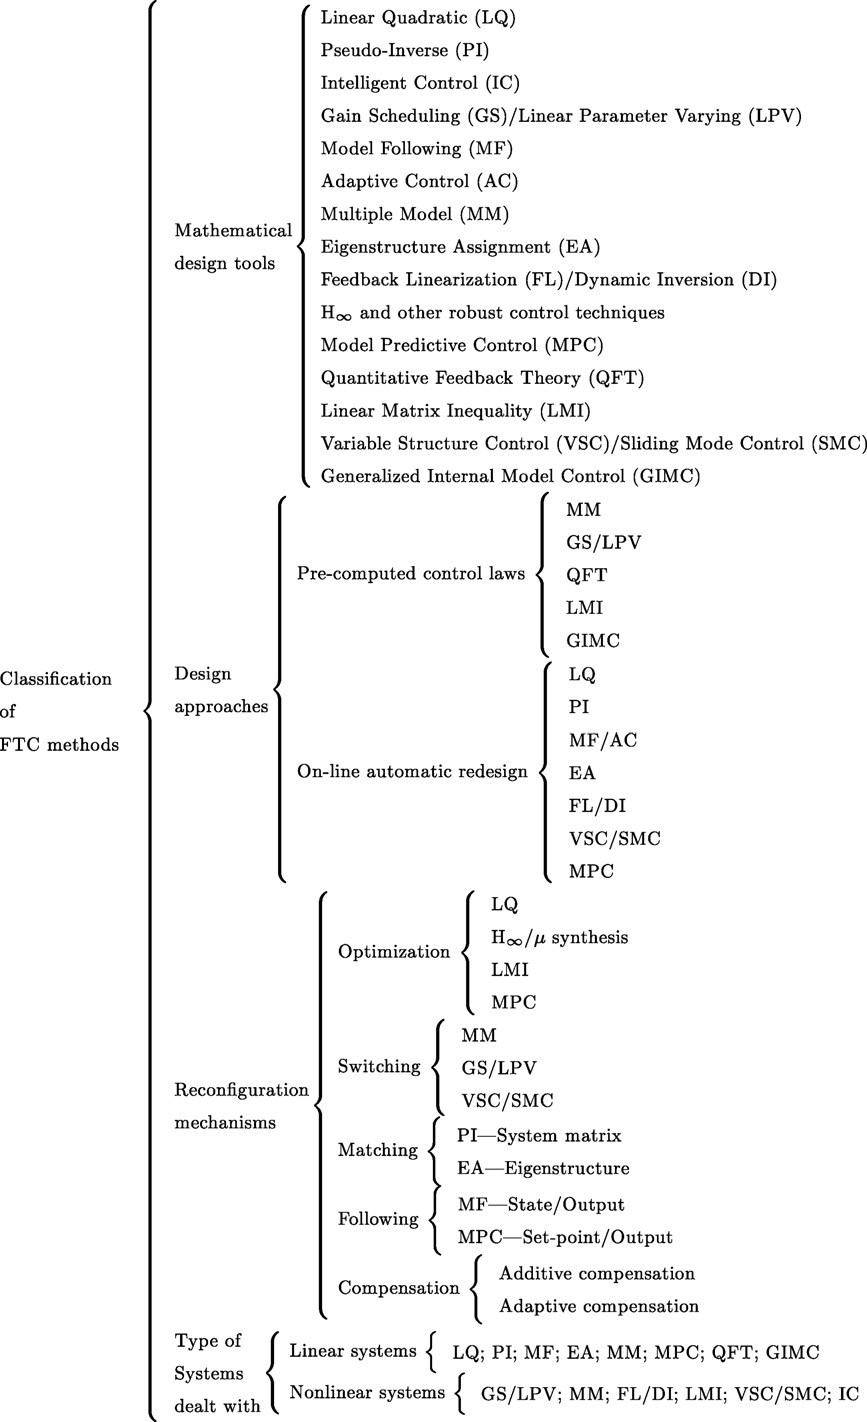
\includegraphics{Reconclass.jpg}
    \bicaption[fig:recclass]{控制器重构方法的分类}{控制器重构方法的分类\cite{Zhang2008229}}{Fig.}{The classification of controller reconfiguration methods}
\end{figure}
结合以上不同的分类,这里主要介绍三类控制器重构的方法——多模型方法、自适应方法和滑模方法。事实上,图\newref{fig:recclass}中提到的10多种方法之间也都有混合与交叉,很少有一种重构方法只依赖一种模型\cite{Zhang2008229}。

\paragraph*{多模型方法}
多模型方法的思路是,用平行的$N$个已知参数的模型来预测系统在不同错误情形下的下一步状态有哪些可能,然后根据测量得到的状态选择一个预测最准确的模型作为参考模型,预测的工具通常使用卡尔曼滤波器。事先给每个模型设计好控制器,一旦确定了错误种类,就立即将控制器切换成该种模型对应的控制器。这种故障重构机制没有在线计算的过程,控制器都是提前设计好的,模型也是提前根据不同错误类型构建的。因此理论上有多少种模型就能够处理多少种错误。

这一类方法主要有两种\cite{5282515}:多模型自适应估计(Multiple model adaptive estimation, MMAE)\cite{81428,70412}与交互多模型(Interacting multiple model, IMM)\cite{976961,827910},其中后者是为了解决系统参数变化的问题而提出的。此外,在飞行器的容错控制领域还有其他基于多模型方法的容错设计,如文献\cite{827910,786187,JUNG2005115}。

\paragraph*{自适应方法}
自适应控制器重构方法\cite{1709933,6670789,7353144}是最为常见的控制器重构策略。Boskovic\cite{703075}对控制输入变量大于控制输出变量的控制器提出了一种自适应控制器重组的方法,在多执行机构卡顿的情况,并且控制器不知道错误信息的情况下能够保持系统稳定。Chen\cite{989090}提出了一种处理输入信号卡顿的控制方法,并给出了针对执行器故障的补偿条件。Zuo\cite{6945860}针对线性和非线性但满足Lipschitz条件的多智能体系统提出了自适应容错控制。自适应方法也通常与神经网络\cite{6060930,Lin2017}、滑模控制\cite{6060930,7506323}、反演(Backstepping)\cite{Li2016177,Jiang201057}、模糊控制\cite{Zou201110}等其他方法结合使用。

\section{当前研究存在的问题}
当前针对容错控制的研究虽然有很多,但是由于平流层飞艇的特殊性,一般的容错控制方案并不能满足其需要。具体来说,平流层飞艇主要有如下特殊之处:
\begin{enumerate}
  \item 平流层飞艇由于内部充气,并工作在空气稀薄的环境下,因此昼夜温差巨大,所以其模型中的惯性矩阵和气动系数在不同时间将会急剧变化。
  \item 平流层飞艇受限于其载重限制,因此执行机构通常远远不能满足控制需要,饱和现象经常出现,需要在容错控制器的设计中考虑到。
  \item 平流层飞艇通常需要长时间工作在临近空间的恶劣环境下\cite{fenggui2013},因此其执行机构非常容易出现卡顿、失效等故障。一般的应对执行机构卡顿的方法。
  \item 平流层飞艇容易受到风的干扰,除此之外还会受到各种不稳定的气流,造成实际故障无法准确跟踪。
  \item 传统的Super-Twisting观测器应用于平流层飞艇进行故障重构的时候,其收敛速度非常缓慢,不能应用于实际中。
\end{enumerate}
因此,在实际中,平流层飞艇会遇到一些以前的研究没有考虑到的问题。所以针对平流层飞艇的研究不能完全采用一般的针对非线性系统的容错控制研究方案,需要单独针对平流层飞艇的模型设计控制方案或者故障重构方案。

\section{本课题创新点}
本课题主要针对浮空器经常出现的一些不确定性、故障和控制难点进行了容错控制器设计。本文的研究内容和创新点主要分为三个部分,分别是:
\begin{enumerate}
    \item 针对平流层飞艇的惯性矩阵和气动矩阵的不确定性,设计了一种自适应滑模容错控制方案。
    \item 针对平流层飞艇的惯性矩阵、气动矩阵的不确定性以及执行机构的效率损失和输出偏移等故障,设计了一种自适应滑模容错控制方案。
    \item 针对Super-Twisting观测器应用于平流层飞艇收敛速度慢的问题,提出了一种改进的Super-twisting观测器,增加了使其收敛速度可调节的参数,并证明了新观测器的稳定性。
\end{enumerate}

\chapter{浮空器数学模型与故障分析}\label{chap:preliminary}
在推导浮空器的容错控制算法时,遇到的首要问题就是如何将浮空器的各项故障表达成数学形式并体现在模型中。本章中给出了本文所使用的浮空器数学模型,和浮空器平时可能遇到的一些常见故障及其数学表达。
\section{浮空器数学模型}
本文所研究的浮空器为外观型如图\newref{fig:airshipoverview}所示的螺旋桨矢量推进的浮空器。其横截面是四段欧拉螺线(Euler Spiral,又称羊角螺线)的一部分围成的闭合图形(图),这样能够保证体积一定的情况下所用布料最少。四个矢量推进螺旋桨均匀分布在最大半径纬度的周围。
\begin{figure}
    \centering
    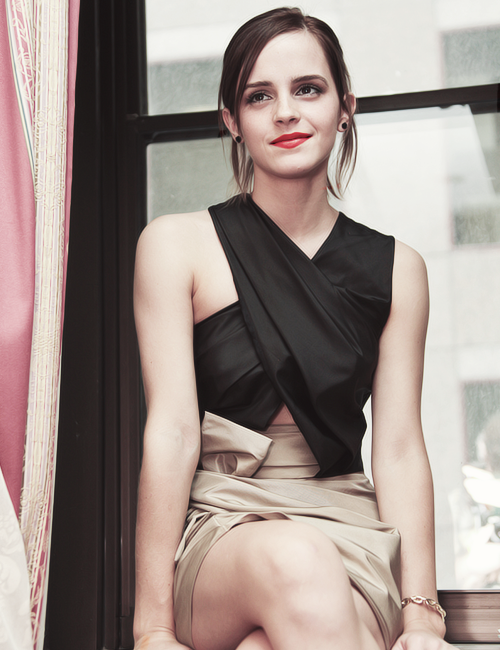
\includegraphics[width=0.5\textwidth]{figure/placeholder.png}
    \bicaption[fig:blimpcut]{欧拉螺线及浮空器横截面}{欧拉螺线及浮空器横截面}{Fig.}{Euler Spiral and Airship Cross-section}
\end{figure}

其机体坐标系、地面坐标系的建立过程和特性和模型已经在文献\citen{Chen20131748,zhanghao2014}中做了详细分析。相关参数也已经在本文前的符号列表中给出,这里仅简单将数学模型简单列举。
\begin{figure}
    \centering
    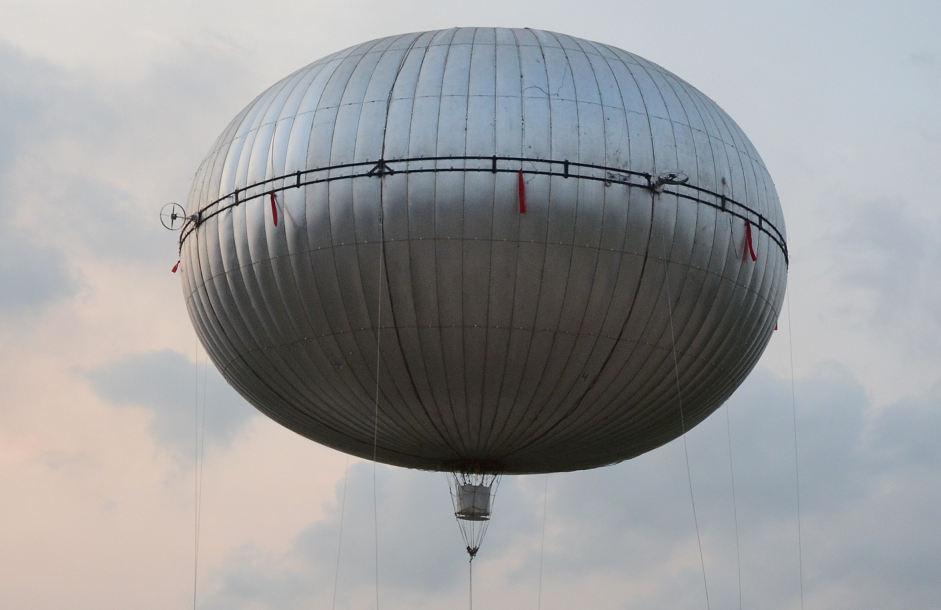
\includegraphics[width=0.7\textwidth]{airship.png}
    \bicaption[fig:airshipoverview]{螺旋桨矢量推进浮空器外观}{螺旋桨矢量推进浮空器外观}{Fig.}{The Apperance of Airship}
\end{figure}

令$x$, $y$, $z$分别为浮空器在地面坐标系下在$x$, $y$, $z$方向的位移,$\mathbf{x_1}=[x,y,z,\phi,\theta,\psi]^T$, $\mathbf{x_2}=[u,v,w,p,q,r]^T$,那么浮空器模型的状态空间形式为
\begin{equation}\label{eq:model1}
    \begin{cases}
    \dot{\mathbf{x}}_1 &= \mathbf{J}\dot{\mathbf{x}}_2 \\
    \mathbf{M}\dot{\mathbf{x}}_2 &= \mathbf{F_{gb}} + \mathbf{F_a} + \mathbf{F_i} + \mathbf{F_t}
    \end{cases}
\end{equation}
其中$\mathbf{J}$是坐标转换矩阵,其表达式为
\begin{equation}\label{eq:J}
\mathbf{J} = \left[\begin{matrix}
\mathbf{J_1}&\mathbf{O_{3\times3}}  \\
\mathbf{O_{3\times3}}&\mathbf{J_2} 
\end{matrix}\right]
\end{equation}

\begin{equation}\label{eq:J1}
\mathbf{J_1}=\left[
\begin{matrix}
\cos\psi\cos\theta&\cos\psi\sin\theta\sin\phi-\sin\psi\cos\phi&\cos\psi\sin\theta\cos\phi+\sin\psi\sin\phi\\
\sin\psi\cos\theta&\sin\psi\sin\theta\sin\phi+\cos\psi\cos\phi &\sin\psi\sin\theta\cos\phi-\cos\psi\sin\phi \\
-\sin\theta &\cos\theta\sin\phi&\cos\theta\cos\phi
\end{matrix}
\right]
\end{equation}

\begin{equation}\label{eq:J2}
\mathbf{J_2}=\left[
\begin{matrix}
1&\sin\phi\tan\theta&\cos\phi\tan\theta  \\
0&\cos\phi&-\sin\phi  \\
0&\sin\phi\sec\theta&\cos\phi\sec\theta  \\
\end{matrix}
\right]
\end{equation}

$\mathbf{M}$是惯性矩阵,其表达式为:
\begin{equation}\label{eq:M}
\mathbf{M}=\left[
\begin{matrix}
m+m_{11}&0&0&0&mz_G&-my_G  \\
0&m+m_{22}&0&0-mz_G&0&mx_G  \\
0&0&m+m_{33}&my_G&-mx_G&0  \\
0&-mz_G&my_G&I_x+m_{44}&0&0  \\
mz_G&0&-mx_G&0&I_y+m_{55}&0  \\
-my_G&mx_G&0&0&0&I_z+m_{66}  \\
\end{matrix}
\right]
\end{equation}

科氏力$\mathbf{F_i}$的表达式为
\begin{equation}\label{eq:Fi}
\mathbf{F_{i}}=\left[
\begin{matrix}
-(m+m_{33})wq+(m+m_{22})vr-mz_Gpr+mx_G(r^2+q^2)-my_Gpq  \\
-(m+m_{11})ur+(m+m_{33})wp-mz_Gqr+my_G(r^2+p^2)-mx_Gpq \\
-(m+m_{22})vp+(m+m_{11})uq-my_Gqr+mz_G(p^2+q^2)-mx_Gpr \\
(m_{55}-m_{66}-I_z+I_y)qr-my_G(pv-qu)+mz_G(ru-pw) \\
(m_{66}-m_{44}-I_x+I_z)pr-mz_G(qw-rv)+mx_G(pv-qu) \\
(m_{44}-m_{55}-I_y+I_z)qp-mx_G(ru-pw)+my_G(qw-rv)
\end{matrix}
\right]
\end{equation}

空气动力$\mathbf{F_a}$的表达式为
\begin{equation}\label{eq:Fa}
\mathbf{F_{a}}=\left[
\begin{matrix}
f_a\cdot\cos\Omega \\
f_a\cdot\sin\Omega \\
q_{\infty}\cdot C_z\cdot S_{ref} \\
-M_a\cdot\cos\Omega \\
M_a\cdot\sin\Omega \\
0\\
\end{matrix}
\right]
\end{equation}
其中
\begin{eqnarray}\label{eq:fa}
f_a &=& q_{\infty}\cdot C_x\cdot  S_{ref} \\
M_a &=& q_{\infty}\cdot C_{my}\cdot  S_{ref} \cdot L_{ref}
\end{eqnarray}

重力与浮力的合力$\mathbf{F_{gb}}$的表达式为
\begin{equation}\label{eq:Fgb}
\mathbf{F_{gb}}=\left[
\begin{matrix}
-(G-B)\mathrm{sin}\theta  \\
(G-B)\mathrm{sin}\phi\mathrm{cos}\theta \\
(G-B)\mathrm{cos}\phi\mathrm{cos}\theta \\
-(Gz_{G}-Bz_{B})\mathrm{sin}\phi\mathrm{cos}\theta \\
-(Gz_{G}-Bz_{B})\mathrm{sin}\theta-(Gx_{G}-Bx_{B})\mathrm{cos}\phi\mathrm{sin}\theta \\
(Gx_{G}-Bx_{B})\mathrm{sin}\phi\mathrm{cos}\theta
\end{matrix}
\right]
\end{equation}

浮空器的控制输入矢量$\mathbf{F_t}=[f_x, f_y, f_z, m_x, m_y, m_z]^T$的推导在文献\citen{zhanghao2014}中有详细提及。如果定义螺旋桨推力向上(即$z$轴负方向)的方向角为$0$,$\mu$为螺旋桨的方位角,其范围为$[-\pi,\pi]$,$f_i\text{ }(i=1,2,3,4)$为四个螺旋桨分别产生的推力大小。在矢量平面内,几个螺旋桨推进器的矢量推力可以分解为水平和垂直方向正交的两个力$f_{iH}$和$f_{iV}$,它们与矢量推力大小、矢量转角的关系为:
\begin{eqnarray}
f_{iH}&=&f_i\sin\mu_i \\
f_{iV}&=&-f_i\cos\mu_i
\end{eqnarray}
将$f_{iH}$和$f_{iV}$分解到坐标轴上,得到六维推力和推力力矩,如图\newref{fig:controlalloc}所示。
\begin{figure}
    \centering
    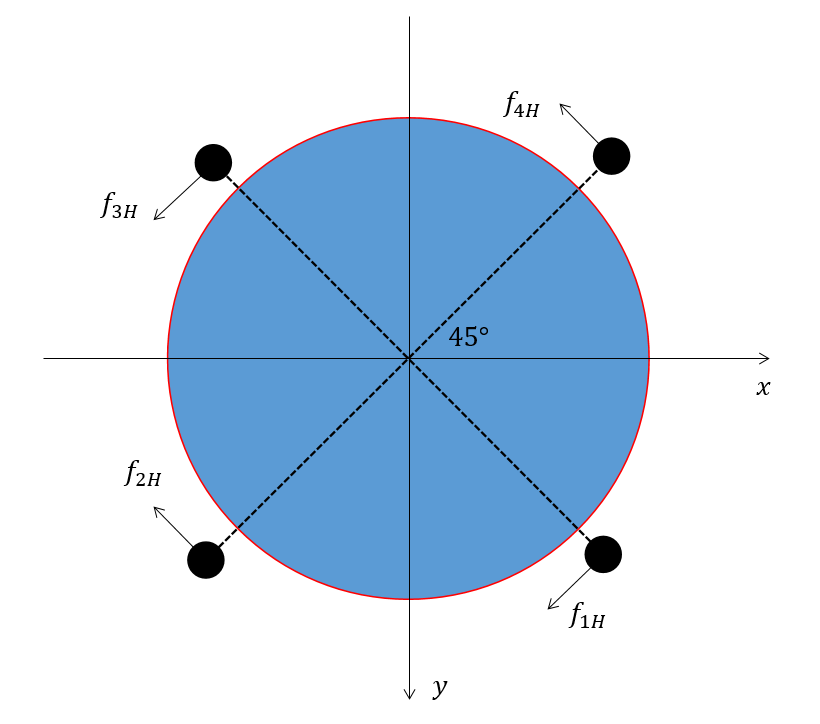
\includegraphics[width=0.7\textwidth]{figure/controlallocation.png}
    \bicaption[fig:controlalloc]{矢量推力局部坐标系和矢量角度定义}{矢量推力局部坐标系和矢量角度定义\cite{zhanghao2014}}{Fig.}{A sketch of the vectored thrusts}
\end{figure}
文献\citen{zhanghao2014}对$\mathbf{F_t}$和$f_{iH}$, $f_{iV}$, $\mu_i$之间的关系进行了详细的推导,这里仅给出结论如下:
\begin{equation}
    \mathbf{F_t}=\mathbf{D}F_{HV}
\end{equation}
其中
\begin{equation}\label{eq:D}
    \mathbf{D}=\left[\begin{matrix}
\rtwo&\rtwo&-\rtwo&-\rtwo&0&0&0&0\\
-\rtwo&\rtwo&\rtwo&-\rtwo&0&0&0&0\\
0&0&0&0&1&1&1&1\\
0&0&0&0&\rtwo R_p&\rtwo R_p&-\rtwo R_p&-\rtwo R_p\\
0&0&0&0&-\rtwo R_p&\rtwo R_p&\rtwo R_p&-\rtwo R_p\\
-R_p&-R_p&-R_p&-R_p&0&0&0&0\\
\end{matrix}
\right]
\end{equation}

\begin{equation}
    F_{HV} = \left[\begin{matrix}f_{1H}&f_{2H}&f_{3H}&f_{4H}&f_{1V}&f_{2V}&f_{3V}&f_{4V}\end{matrix}
\right]^T
\end{equation}

这里$\mathbf{D}$为控制分配矩阵,$F_{HV}$为中间控制量。

在实际进行控制时,控制器计算得出控制量$\mathbf{F_t}$后,通过$\mathbf{D}$的伪逆矩阵$\mathbf{D}^{\dagger}$和\neweqref{eq:fthv}可以计算得出每个螺旋桨实际需求的分力$F_{T_{HV}}$,再通过\neweqref{eq:fi}和\neweqref{eq:miui}计算出各个螺旋桨的实际输出量,求得每个螺旋桨实际所需的推力和转角大小。
\begin{equation}\label{eq:fthv}
    F_{T_{HV}} = \mathbf{D}^{\dagger}\mathbf{F_t}
\end{equation}

\begin{equation}\label{eq:fi}
    f_i = \sqrt{f_{iH}^2+f_{iV}^2}, \qquad (i=1,2,3,4)
\end{equation}

\begin{equation}\label{eq:miui}
    \mu_i = \tan^{-1}\left(\frac{f_{iH}}{f_{iV}}\right), \qquad (i=1,2,3,4)
\end{equation}

\section{浮空器故障的数学形式分析}
\subsection{附加质量问题}
不同于高速飞行器,浮空器的附加质量非常明显。事实上,任何在流体中运动的物体都会对流体产生作用力,这个作用力会对物体本身产生反作用力,造成物体的动量变化\cite{mueller2004development}。为了仍使物体维持原定速度运行,人们引入了附加质量来抵消这部分流体反作用力。在传统的飞机模型中,因为飞机本身质量很大,这部分空气反作用力是可以被忽略的。然而对于浮空器来说,这部分反作用力和其质量几乎同属一个数量级,因此不能被忽略。

附加质量的数学形式就体现在惯性矩阵$\mathbf{M}$中。如果没有附加质量,那么浮空器的惯性矩阵应为对角阵:
\begin{equation}
    \left[\begin{matrix}
    m&&&&&\\
    &m&&&&\\
    &&m&&&\\
    &&&I_x&&\\
    &&&&I_y&\\
    &&&&&I_z\\
    \end{matrix}\right]
\end{equation}

引入附加质量后,需要注意的是每个飞行器的惯性矩阵都因其形状而各自不同,式\neweqref{eq:M}所示的附加质量矩阵只适用于本文的或与本文中研究对象形状相似的物体。

\subsection{气动参数不确定问题}
气动参数不确定也是浮空器研究中经常面临的一类问题。这里的气动参数主要指式\neweqref{eq:Fa}-\neweqref{eq:fa}中的参数$C_x$, $C_z$和$C_{my}$。这几个参数与浮空器当前的气动迎角$\Omega$有关,通常测量方法是在风洞中每隔一段角度测出对应迎角的气动系数,得到一个参数表。对于某一未测量角度的气动参数,则是根据已知的参数表进行线性插值求得。这样获取的气动参数的不准确性在于

\begin{itemize}
    \item 由于风速不确定的原因,实际的迎角不易准确测得。
    \item 即使迎角可以准确测到,由于浮空器的形变等原因,其气动系数相对于风洞中的测量值可能会有变化。
    \item 由于在风洞中不可能对每个角度都进行测量,因此在对气动系数进行线性插值时会产生误差。
\end{itemize}

以上原因造成了实际中使用的$C_x$,$C_z$与$C_{my}$都会与真实值有出入,因此气动参数不确定也是浮空器研究面临的一个难点。在本文的后续仿真中,我们以增加一个正态分布扰动来表示真实的气动系数。

\subsection{外部扰动问题}
外部扰动指的是除了已知的控制输入外,空气额外作用在浮空器上的力。对于浮空器来说,通常最大的外部扰动来源是风的影响,同时也可能有一些湍流等作用。外部扰动分为匹配(matched)扰动和不匹配(unmatched)扰动。匹配扰动表示可以将这部分扰动归并到执行机构扰动中考虑,并在执行机构中做相应的补偿就可以了;而不匹配扰动则无法通过执行机构做直接补偿。浮空器的外部扰动的数学模型是在模型\neweqref{eq:model1}中的动力学方程中直接添加,即

\begin{equation}
    \mathbf{M}\dot{\mathbf{x}}_2 = \mathbf{F_{gb}} + \mathbf{F_a} + \mathbf{F_i} + \mathbf{F_t} + \mathbf{d}
\end{equation}

其中$\mathbf{d}$为外部扰动。

\subsection{执行机构故障}
执行机构故障也是一种常见的系统错误。由于平流层浮空器通常工作在十分恶劣的环境下,因此任何执行机构,包括螺旋桨和舵面,都很容易失效。由于本文的研究对象的执行机构是螺旋桨,所以本文仅给出了针对螺旋桨一些常见故障的数学建模。

螺旋桨遇到的问题可以归结为效率损失、输出偏移,卡顿和失效等几类。假设某个执行机构$i$的期望输出为$\upsilon_i$, 其输出效率为$\varepsilon_i$,输出偏移为$\bar{\upsilon_i}$,那么有
\begin{equation}\label{eq:outputeff}
    u_{ai} = \varepsilon_i(t)\upsilon_i+\bar{\upsilon_i}
\end{equation}

对于上述提到的各种故障,可总结其数学模型于表\newref{tab:faultmodel}。
\begin{table}[ht]
    \centering
	\bicaption[tab:faultmodel]{螺旋桨故障及其数学模型}{螺旋桨故障及其数学模型}{Table}{Thrust fault classifications and math models}
	\vspace{0.5em}
	\begin{tabular}{lll}
		\toprule
		故障类型&$\varepsilon_i(t)$&$\bar{\upsilon}_i$ \\
		\midrule
		正常&$\varepsilon_i(t)=1$&$\bar{\upsilon}_i=0$\\
		效率损失&$\varepsilon_i(t)<1$&$\bar{\upsilon}_i=0$\\
		输出偏移&$\varepsilon_i(t)=1$&$\bar{\upsilon}_i\neq0$\\
		卡顿&$\varepsilon_i(t)=0$&$\upsilon_i\neq0$\\
		失效&$\varepsilon_i(t)=0$&$\upsilon_i=0$\\
		\bottomrule
	\end{tabular}
\end{table}

浮空器的实际输出$\mathbf{F_t}$可用式\neweqref{eq:inputtrans}表示

\begin{equation}\label{eq:inputtrans}
    \mathbf{F_t} = \mathbf{Du_a} = \mathbf{D}[EF_{HV} + \bar{\upsilon}]
\end{equation}

其中

\begin{equation*}
    E = \left[\begin{matrix}
    \varepsilon_1&&&&&&&\\
    &\varepsilon_2&&&&&&\\
    &&\varepsilon_3&&&&&\\
    &&&\varepsilon_4&&&&\\
    &&&&\varepsilon_5&&&\\
    &&&&&\varepsilon_6&&\\
    &&&&&&\varepsilon_7&\\
    &&&&&&&\varepsilon_8\\
    \end{matrix}\right]
\end{equation*}

\begin{equation*}
    \bar{\upsilon} = \left[\begin{matrix}
    \bar{\upsilon}_1&\bar{\upsilon}_2&\cdots&\bar{\upsilon}_8
    \end{matrix}\right]^T
\end{equation*}


\section{本章小结}
本章简要介绍了本文的研究对象浮空器的形状。同时引入了浮空器数学模型和它不同于飞机的独特之处。在第二节中介绍了浮空器运行时可能遇到的各类故障和扰动、以及它们在浮空器模型方程中的数学体现,为后文设计浮空器的容错控制算法做了坚实的铺垫,打下了良好的基础。
%# -*- coding: utf-8-unix -*-
%%==================================================
%% chapter01.tex for SJTU Master Thesis
%%==================================================

%\bibliographystyle{sjtu2}%[此处用于每章都生产参考文献]
\chapter{一种基于自适应滑模方法的抗参数扰动的容错控制策略}
\label{chap:asmcsat}
\section{引言}
作为一种轻于空气的飞行器,浮空器在平流层的稳定能力是评价其性能的重要标准。然而,如第\newref{chap:preliminary}章所介绍,浮空器特有的高附加质量和气动参数不准确问题,给它的稳定控制增加了很大的困难。在近期的研究中,曾经有针对航空器采用自适应控制的策略应对质量矩阵不确定性的研究,如\cite{7061535}。文献\cite{7978124}针对浮空器不停变化的气动力设计了一个非线性扰动观测器,以此来抵消气动系数不确定的影响。但是目前在浮空器上同时考虑质量矩阵不确定和气动系数的研究仍然缺乏。本章结合了自适应控制与滑模控制各自的优点,提出了一种新的自适应率,并设计了一种新的容错控制器,能够使得浮空器在质量矩阵扰动和气动系数扰动都未知的情况下仍然保持姿态和位置稳定。同时,考虑到实际情况,还引入了一种执行机构抗饱和策略。

\section{问题表述}
式\neweqref{eq:model1}所示的浮空器模型如下
\begin{equation*}
    \begin{cases}
    \dot{\mathbf{x}}_1 &= \mathbf{J}\mathbf{x}_2 \\
    \mathbf{M}\dot{\mathbf{x}}_2 &= \mathbf{F_{gb}} + \mathbf{F_a} + \mathbf{F_i} + \mathbf{F_t}
    \end{cases}
\end{equation*}

为了书写方便,这里将气动力矩阵$\mathbf{F_a}$写成参数分离的形式,即
\begin{equation}\label{eq:Fa-para}
    \mathbf{F_a} = \mathbf{S}(\mathbf{x}_2)\mathbf{c}
\end{equation}
其中
\begin{equation}\label{eq:Sx2}
\mathbf{S(x_2)}=\left[
\begin{matrix}
q_\infty\cdot S_{ref}\cdot\cos\Omega&0&0 \\
q_\infty\cdot S_{ref}\cdot\sin\Omega&0&0  \\
0&q_\infty\cdot S_{ref}&0  \\
0&0&-q_\infty\cdot S_{ref}\cdot L_{ref}\cdot \cos\Omega  \\
0&0&-q_\infty\cdot S_{ref}\cdot L_{ref}\cdot \sin\Omega  \\
0&0&0  \\
\end{matrix}
\right]
\end{equation}

\begin{equation}\label{eq:cvector}
    \mathbf{c} = \left[\begin{matrix}
    C_x&C_z&C_{my}
    \end{matrix}\right]^T
\end{equation}

质量矩阵和气动系数都不缺定的情况,表现在模型中,可以假设为
\begin{eqnarray}
    \mathbf{M}&=&\mathbf{M}+\mathbf{M}_{\Delta} \label{eq:Muncertainty} \\
    \mathbf{c}&=&\mathbf{c}+\mathbf{c}_{\Delta} \label{eq:cuncertainty}
\end{eqnarray}

其中$\mathbf{M}_{\Delta}$和$\mathbf{c}_{\Delta}$都是未知扰动。

新的浮空器模型变为
\begin{equation}\label{eq:modelwc}
    \begin{cases}
    \hspace{4.5em}\dot{\mathbf{x}}_1 &= \mathbf{J}\mathbf{x}_2\\
    (\mathbf{M}+\mathbf{M}_{\Delta})\dot{\mathbf{x}}_2&=\mathbf{F_{gb}+F_{i}(x_2)}+\mathbf{S(x_2)} (\mathbf{c}+\mathbf{c}_{\Delta})+\mathbf{F_t}
    \end{cases}
\end{equation}

本章任务是针对浮空器模型\neweqref{eq:modelwc}提出一种控制策略使其保持姿态和位置。

\section{算法详述与稳定性证明}\label{sec:3algo}
为了表述方便,下文用函数$\mathbf{F}(\mathbf{x}_1,\mathbf{x}_2)$指代$\mathbf{F_{gb}+F_{i}(x_2)}+\mathbf{S(x_2)} (\mathbf{c}+\mathbf{c}_{\Delta})$。飞艇的动力学方程变为
\begin{equation}\label{eq:dynamicwc}
    (\mathbf{M}+\mathbf{M}_{\Delta})\dot{\mathbf{x}}_2=\mathbf{F(x_1,x_2)+u}
\end{equation}

选择滑模面
\begin{equation}
    \mathbf{s}(t)=\mathbf{x_2+Cx_1}=0
\end{equation}

这里$\mathbf{C}\in\mathbb{R}^{6\times 6}>0$是收敛参数。在给出控制率之前,我们需要做如下几个假设

\begin{ass}\label{3ass:M}
添加了扰动后的质量矩阵是正定的,并且有一个未知的上限$M_{max}$,不会趋近于无穷大。即
\begin{equation}\label{eq:3assM}
    \lVert\mathbf{M}+\mathbf{M}_{\Delta}\rVert\leqslant M_{max}
\end{equation}
\end{ass}
\begin{ass}\label{3ass:F}
浮空器的重浮力、科氏力和气动力的合力满足
\begin{equation}\label{eq:3assF}
    \bnorm{F(x_1,x_2)}\leqslant k_0+k_1\bnorm{x_1}+k\bnorm{x_2}
\end{equation}
其中$k_0$, $k_1$, $k$为正实数。
\end{ass}
根据假设\newref{3ass:M},可以再做出一个合理假设
\begin{ass}\label{3ass:MCJ}
惯性矩阵$\mathbf{M}$, 惯性矩阵的扰动$\mathbf{M}_{\Delta}$, 滑模面参数矩阵$\mathbf{C}$, 坐标转换矩阵$\mathbf{J}$满足:
\begin{equation}
    \lVert(\mathbf{M}+\mathbf{M}_{\Delta})\mathbf{CJ}\rVert\bnorm{x_2}\leqslant (k_2-k)\bnorm{x_2}
\end{equation}
其中$k_2>k$为正实数。
\end{ass}

\begin{rem}
上述假设\newref{3ass:M}-\newref{3ass:MCJ}都是合理的。对于假设\newref{3ass:M},由于浮空器的惯性矩阵$\mathbf{M}$本身在无附加质量的情况下是正定的,只要附加质量不超过浮空器质量本身,假设\newref{3ass:M}都是能够成立的。而附加质量如果超过质量本身的情况,需要更加复杂的分析,本章不做讨论;假设\newref{3ass:F}和假设\newref{3ass:MCJ}给出的条件都是给不确定性设置了一个上界,不同于传统方法设置常值上界,这里采用浮空器自身的状态变量来设置这个上界,浮空器状态变量的值越大,那么浮空器受到的不确定性也越大,符合实际条件。假设\newref{3ass:F}和\newref{3ass:MCJ}中,假定不确定性的增长不快于浮空器状态变量的线性增长,是为了方便后文的推导。如果选择一些多项式函数或者非线性函数,也可以通过重新选取滑模面或自适应率达到同样的效果。
\end{rem}

基于假设\newref{3ass:M}-\newref{3ass:MCJ},定义控制输入$\mathbf{u}$为
\begin{equation}\label{eq:3input}
\mathbf{u} = -\tau\mathbf{s}(t)-\sigma \mathrm{sign}\,(\mathbf{s}(t)) - \mathbf{u_p}
\end{equation}

其中
\begin{eqnarray}
    \tau &=& \left[\begin{matrix}
         \tau_1&&  \\
         &\ddots& \\
         &&\tau_6
    \end{matrix}\right] \\
    \sigma &=& \left[\begin{matrix}
         \sigma&&  \\
         &\ddots& \\
         &&\sigma
    \end{matrix}\right] \\
    \hat{\rho}&=&\hat{k_0}+\hat{k_1}\bnorm{x_1}+\hat{k_2}\bnorm{x_2} \label{eq:inputrho} \\
    \dot{\hat{k_0}}&=&p_0\bnorm{s} \label{eq:adlaw1} \\
    \dot{\hat{k_1}}&=&p_1\bnorm{s}\bnorm{x_1} \label{eq:adlaw2} \\
    \dot{\hat{k_2}}&=&p_2\bnorm{s}\bnorm{x_2} \label{eq:adlaw3}
\end{eqnarray}

\begin{rem}
控制器\neweqref{eq:3input}由三个部分组成。$\mathbf{u_p}$是用于补偿不确定性的自适应率。$-\tau\mathbf{s}(t)-\sigma \mathrm{sgn}(\mathbf{s}(t))$ 这两项能够保证系统到达滑模面并且持续留在滑模面上。$\tau$和$\sigma$是设计参数,用于控制系统到达滑模面的时间。理论上不论是$-\tau\mathbf{s}(t)$还是$-\sigma \mathrm{sgn}(\mathbf{s}(t))$都足够保证系统的收敛,本文设计控制器的时候流出了一部分冗余参数以适应一些未知情况,也能保证让系统状态更快地收敛到滑模面上。
\end{rem}

下面将证明控制器\neweqref{eq:3input}能够在基于假设\newref{3ass:M}-\newref{3ass:MCJ}的条件下,使得浮空器系统\neweqref{eq:modelwc}稳定。

选取李雅普诺夫函数
\begin{equation}\label{eq:3lyapnov}
    V=\frac{1}{2}\left[\mathbf{s}^T(\mathbf{M}+\mathbf{M}_{\Delta})\mathbf{s}+\frac{1}{p_0}(k_0-\hat{k_0})^2+\frac{1}{p_1}(k_1-\hat{k_1})^2+\frac{1}{p_2}(k_2-\hat{k_2})^2\right]
\end{equation}

对$V$求导,得到
\begin{align}\label{eq:Vdot}
    \dot{V}&=\mathbf{s}^T(\mathbf{M}+\mathbf{M}_{\Delta})\mathbf{s}-\frac{1}{p_0}(k_0-\hat{k_0})\dot{\hat{k_0}}-\frac{1}{p_1}(k_1-\hat{k_1})\dot{\hat{k_1}}-\frac{1}{p_2}(k_2-\hat{k_2})\dot{\hat{k_2}} \nonumber
\\&=\mathbf{s}^T(\mathbf{M}+\mathbf{M}_{\Delta})\mathbf{(C\dot{x}_1+\dot{x}_2)} - \Delta \nonumber
\\&=\mathbf{s}^T(\mathbf{M}+\mathbf{M}_{\Delta})\mathbf{Cx_2}+\mathbf{{s^{T}[F(x_1,x_2)+u]}}-\Delta \nonumber
\\& \leqslant \mathbf{\norm{s}\norm{(M+M_{\Delta})C}\norm{x_2}+\norm{s}\norm{F(x_1,x_2)}}+\mathbf{s^{T}u}-\Delta \nonumber
\\& \leqslant \bnorm{s}[(k_2-k)\norm{\mathbf{x_2}}+(k_0+k_1\norm{\mathbf{x_1}}+k\norm{\mathbf{x_2}})]+\mathbf{s^{T}u}-\Delta \nonumber
\\&=\norm{\mathbf{s}}(k_0+k_1\norm{\mathbf{x_1}}+k_2\norm{\mathbf{x_2}})+\mathbf{s^{T}u}-\Delta 
\end{align}

为书写方便,式\neweqref{eq:Vdot}中
\begin{equation}\label{eq:Delta}
    \Delta = -\frac{1}{p_0}(k_0-\hat{k_0})\dot{\hat{k_0}}-\frac{1}{p_1}(k_1-\hat{k_1})\dot{\hat{k_1}}-\frac{1}{p_2}(k_2-\hat{k_2})\dot{\hat{k_2}}
\end{equation}

注意到
\begin{align}\label{eq:process1}
&\mathbf{s}^T\mathbf{u}-\Delta \nonumber
\\&= \mathbf{s}^T\Big[-\tau\mathbf{s}-\sigma\mathrm{sign}\,(\mathbf{s})-\frac{\mathbf{s}}{\bnorm{s}}(\hat{k_0}+\hat{k_1}\bnorm{x_1}+\hat{k}\bnorm{x_2})\Big]-\Delta \nonumber
\\&=\mathbf{s}^T[-\tau \mathbf{s}-\sigma\mathrm{sgn}(\mathbf{s})]-\bnorm{s}(\hat{k_0}+\hat{k_1}\bnorm{x_1}+\hat{k_2}\bnorm{x_2})-\Delta
\end{align}

设$s_i$为滑模面向量$\mathbf{s}$的各个分量,把\neweqref{eq:Delta}、\neweqref{eq:process1}代入\neweqref{eq:Vdot},可以得到
\begin{align}\label{eq:V<03-1}
    \dot{V}&=\mathbf{s^{T}[-\tau s-\sigma \mathrm{sgn}(s)]} \nonumber\\
    &=\sum_{i=1}^{6}-\tau_is_i^{2}-\sigma_i\abs{s_i}\leqslant0
\end{align}

证毕。
\vspace{1em}

通过\neweqref{eq:V<03-1}式,结合Barbashin-Krasovskii定理\footnote{《非线性系统》\cite{Khalilnonlinearbookchinese},Hassan K. Khalil著,电子工业出版社,2012年版,第124页}可知控制器\neweqref{eq:3input}能够在基于假设\newref{3ass:M}-\newref{3ass:MCJ}的条件下,使得浮空器系统\neweqref{eq:modelwc}稳定。以下推导中$\mathbf{u}$即表示所需控制输入量$\mathbf{F_t}$。

\section{抗饱和策略的引入}\label{sec:3sat}
浮空器在运行时不可避免地会遇到执行机构饱和问题,本节在\newref{sec:3sat}的基础上,对上述控制器\neweqref{eq:3input}进行一些修改,使其能够处理执行机构饱和的问题。

首先需要对执行机构饱和进行数学建模。我们用$\mathbf{u}_{sat}$来代替实际系统考虑饱和后的输入。

此时浮空器系统变为:
\begin{equation}\label{eq:modelwcsat}
    \begin{cases}
    \hspace{4.5em}\dot{\mathbf{x}}_1 &= \mathbf{J}\mathbf{x}_2\\
    (\mathbf{M}+\mathbf{M}_{\Delta})\dot{\mathbf{x}}_2&=\mathbf{F_{gb}+F_{i}(x_2)}+\mathbf{S(x_2)} (\mathbf{c}+\mathbf{c}_{\Delta})+\mathbf{u}_{sat}
    \end{cases}
\end{equation}

而$\mathbf{u}_{sat}$的表达式为

\begin{equation}\label{eq:satu}
    \mathbf{u}_{sat} = \mathbf{E}\mathbf{u}
\end{equation}

这里$\mathbf{u}=[u_1,u_2,\cdots,u_6]^T$是期望输入,$\mathbf{E}$是如下对角矩阵:
\begin{equation*}
    \mathbf{E} = \left[\begin{matrix}
         \varepsilon_1&&  \\
         &\ddots& \\
         &&\varepsilon_6
    \end{matrix}\right] 
\end{equation*}
并满足
\begin{equation*}
    \varepsilon_i = \begin{cases}
    \frac{|u_{mi}|}{|u_i|} & \text{if } u_i>u_{mi}\\
    1 & \text{if } u_i \leqslant u_{mi}
    \end{cases}
\end{equation*}
$u_{mi}$是第$i$个分量的最大输入,$0<\varepsilon_i<1$。

此外,\newref{sec:3algo}节中的假设条件需要变动为如下两个假设条件:

\begin{ass}\label{3ass:sat1}
浮空器的重浮力、科氏力和气动力的合力满足
\begin{equation}\label{eq:3asssat1}
    \bnorm{F(x_1,x_2)}\leqslant m_0\bnorm{x_2}
\end{equation}
其中$m_0$为正实数。
\end{ass}

\begin{ass}\label{3ass:sat2}
惯性矩阵$\mathbf{M}$, 惯性矩阵的扰动$\mathbf{M}_{\Delta}$, 滑模面参数矩阵$\mathbf{C}$, 坐标转换矩阵$\mathbf{J}$满足:
\begin{equation}\label{eq:3asssat2}
    \lVert(\mathbf{M}+\mathbf{M}_{\Delta})\mathbf{CJ}\rVert\bnorm{x_2}\leqslant (m-m_0)\bnorm{x_2}
\end{equation}
其中$m$为正实数,并满足$m>m_0$。
\end{ass}

为证明方便,先引入如下引理
\begin{lem}\label{lm:chap3}
    若$\mathbf{x}=\left[\begin{matrix}x_1&x_2&\cdots&x_n\end{matrix}\right]^T$是一个$n\times 1$的向量,$A$是一个$n\times n$的对角矩阵且满足$A=diag(a_1,a_2,\cdots,a_n)\text{,}(0<a_i<1)$。$k$是一个正实数标量,$a_{low}$是$a_1,\cdots,a_n$中最小的元素,那么有如下结论:
    \begin{equation}
        \mathbf{x}^TAk\mathbf{x}\geqslant ka_{low}\bnorm{\mathbf{x}}^2
    \end{equation}
\end{lem}

\begin{proof}
    \begin{align}
    \mathbf{x}^TAk\mathbf{x} &= \sum_{i=1}^n ka_ix_i^2 \nonumber\\
    &\geqslant \sum_{i=1}^n ka_{low}x_i^2 \nonumber\\
    &= ka_{low}\sum_{i=1}^n x_i^2 \nonumber\\
    &= ka_{low}\bnorm{\mathbf{x}}^2  
    \end{align}
    证毕。
\end{proof}

根据假设\newref{3ass:sat1}和\newref{3ass:sat2},定义控制率

\begin{equation}\label{eq:inputsat}
\mathbf{u}_{sat} = -\tau\mathbf{s}(t)-\sigma \mathrm{sign}\,(\mathbf{s}(t)) - \mathbf{u_s}
\end{equation}

其中
\begin{eqnarray}
        \tau &=& \left[\begin{matrix}
         \tau_1&&  \\
         &\ddots& \\
         &&\tau_6
    \end{matrix}\right] \nonumber\\
    \sigma &=& \left[\begin{matrix}
         \sigma&&  \\
         &\ddots& \\
         &&\sigma
    \end{matrix}\right] \nonumber\\
    \mathbf{u_s}&=&\frac{\hat{\beta}\hat{m}\bnorm{x_2}\mathbf{s}}{\bnorm{s}} \\
    \dot{\hat{m}} &=& p_3\bnorm{s}\bnorm{x_2} \label{eq:updatead1} \\
    \dot{\hat{\beta}} &=& \hat{\beta}^3\hat{m}\bnorm{s}\bnorm{x_2} \label{eq:updatead2}
\end{eqnarray}

下面证明,控制率\neweqref{eq:inputsat}在假设\newref{3ass:sat1}和\newref{3ass:sat2}的条件下,能够使得浮空器饱和输入模型\neweqref{eq:modelwcsat}保持稳定。

首先,选取一个标量$\xi$满足
\begin{equation}\label{eq:choosexi}
    0<\xi<\mbox{min}\{\varepsilon_1,\varepsilon_2,\cdots,\varepsilon_6\}<1
\end{equation}

定义李雅普诺夫函数
\begin{equation}\label{eq:lyapads}
    V_s=\frac{1}{2}\left[\mathbf{s^T(M+M_{\Delta})s}+\frac{1}{p_3}\tilde{m}^2+\frac{1}{p_4}\tilde{\beta}^2\right]
\end{equation}
其中$\tilde{m}=m-\hat{m}$,$\tilde{\beta}=\xi-\frac{1}{\hat{\beta}}$。

显然可得$\dot{\tilde{m}}=-\dot{\hat{m}}$ 和 $\dot{\tilde{\beta}}=\frac{\dot{\hat{\beta}}}{\hat{\beta}^2}$

对$V_s$求导,得到
\begin{align}
    \dot{V}_s &= \mathbf{s}^T(\mathbf{M}+\mathbf{M}_{\Delta})\mathbf{s} + \frac{1}{p_3}\tilde{m}\dot{\tilde{m}}+\frac{1}{p_4}\tilde{\beta}\hat{\tilde{\beta}} \nonumber\\
&=\mathbf{s}^T(\mathbf{M}+\mathbf{M}_{\Delta})\mathbf{(\dot{x}_2+Cx_2)}-\frac{\tilde{m}\dot{\hat{m}}}{p_3}+\frac{\tilde{\beta}\dot{\hat{\beta}}}{p_4\hat{\beta}^2} \nonumber\\
&= \mathbf{s}^T(\mathbf{M}+\mathbf{M}_{\Delta})\mathbf{Cx_2}+\mathbf{s^T}(\mathbf{F}+\mathbf{u}_{sat})-\tilde{m}\bnorm{s}\bnorm{x_2}+\tilde{\beta}\hat{\beta}\hat{m}\bnorm{s}\bnorm{x_2} \nonumber\\
&\leqslant \bnorm{s}(m-m_0)\bnorm{x_2}+m_0\bnorm{s}\bnorm{x_2}+\mathbf{s^TEu}-\tilde{m}\bnorm{s}\bnorm{x_2}+\tilde{\beta}\hat{\beta}\hat{m}\bnorm{s}\bnorm{x_2} \nonumber\\
&=\mathbf{s^TE}(-\tau\mathbf{s}(t)-\sigma \mathrm{sign}\,(\mathbf{s}(t)) - \mathbf{u_s})+\hat{m}\bnorm{s}\bnorm{x_2}+\tilde{\beta}\hat{\beta}\hat{m}\bnorm{s}\bnorm{x_2} \nonumber\\
&= \mathbf{s^TE}(-\tau\mathbf{s}(t)-\sigma \mathrm{sgn}(\mathbf{s}(t)))-\mathbf{s^TEu_s}+\hat{m}\bnorm{s}\bnorm{x_2}+(\xi-\frac{1}{\hat{\beta}})\hat{\beta}\hat{m}\bnorm{s}\bnorm{x_2} \nonumber\\
&=-\sum_{i=1}^6(\varepsilon_i\tau_is_i^2-\varepsilon_i\sigma_i|s_i|)-\mathbf{s^TE}\frac{\hat{\beta}\hat{m}\bnorm{x_2}\mathbf{s}}{\bnorm{s}}+\xi\hat{\beta}\hat{m}\bnorm{s}\bnorm{x_2} \label{eq:lypaad1}
\end{align}

由引理\newref{lm:chap3},可得
\begin{align}
    \mathbf{s^TE}\frac{\hat{\beta}\hat{m}\bnorm{x_2}}{\bnorm{s}}\mathbf{s} &\geqslant \frac{\hat{\beta}\hat{m}\bnorm{x_2}}{\bnorm{s}}\varepsilon_{low}\bnorm{s}^2> \xi\hat{\beta}\hat{m}\bnorm{s}\bnorm{x_2}
\end{align}

继续由\neweqref{eq:lypaad1}得
\begin{equation}
    \dot{V}_s<-\sum_{i=1}^6(\varepsilon_i\tau_is_i^2+\varepsilon_i\sigma_i|s_i|)
\end{equation}

因为$\varepsilon_i, \sigma_i, \tau_i\text{  (i$\in$\{1,2,$\cdots$,6\})}$都是正实数,因此可得$\dot{V}_s<0$,证毕。
\vspace{1em}

因此,控制率\neweqref{eq:inputsat}在假设\newref{3ass:sat1}和\newref{3ass:sat2}的条件下,能够使得浮空器饱和输入模型\neweqref{eq:modelwcsat}保持稳定。

\section{数值仿真与对比}
在本节中,我对\newref{sec:3algo}和\newref{sec:3sat}提到的算法进行了仿真。在给出仿真结果前,表\newref{tab:para}中给出了一些必要的浮空器参数。

\begin{table}[!htp]
  \centering
  \bicaption[tab:para]{浮空器模型参数}{浮空器模型参数}{Table}{Airship model parameters}
  \vspace{0.5em}
  \begin{tabular}{cl}
    \toprule
    参数&值\\
    \midrule
    $m(kg)$&72\\
    $m_{11}(kg)$&10.8147\\
    $m_{22}(kg)$&10.8147\\
    $m_{33}(kg)$&38.9521\\
    $m_{44}(kg)$&19.3024\\
    $m_{55}(kg)$&19.3024\\
    $m_{66}(kg)$&0\\
    $I_x(kg\cdot m^2)$&409.4260\\
    $I_y(kg\cdot m^2)$&409.4260\\
    $I_z(kg\cdot m^2)$&34.5941\\
    $R_p(m)$&2.81\\
    $(x_G,y_G,z_G)(m)$&(0,0,2)\\
    \bottomrule
  \end{tabular}
\end{table}

为了更直观地说明算法的效果,本文同时也给出了D. Han论文中针对浮空器设计的自适应反演(Adaptive Backsteppting, ABS)算法\cite{han2015adaptive}和Y. Yang论文中\cite{Yang2016Positioning}针对浮空器设计的反演滑模(Backstepping Sliding Mode Control, BSMC)位置控制算法的结果进行对比。需要注意的是,Y. Yang论文中的算法是针对一个三自由度模型设计的,我们仿真的时候用它来对六自由度模型进行控制,其结果是不可预测的。

对于仿真中用到的参数说明如下:滑模参数选取为$\tau=2\mathbf{I_6}$, $\sigma=0.001\mathbf{I_6}$ 和 $\mathbf{C}=0.3\mathbf{I_6}$,其中$\mathbf{I}_6$是$6\times 6$的单位矩阵。自适应率中的参数$p_0=p_1=p_2=p_3=p_4=1$。各个自适应变量的初值为$\hat{k}_0(0)=\hat{k}_1(0)=\hat{k}_2(0)=\hat{m}(0)=\hat{\beta}(0)=0.001$。每个螺旋桨的最大推力设置为110N。本节仿真主要分为如下几个部分:
\begin{description}
    \item[仿真1:两组无参数扰动情况] 对照组,选取$\mathbf{M}_{\Delta}=\mathbf{c}_{\Delta}=0$,使用\newref{sec:3algo}节的算法、D. Han的算法以及Y. Yang的算法对两组初值进行仿真对比,仿真时长40秒。
    \item[仿真2:\newref{sec:3algo}节算法有扰动] 对于\newref{sec:3algo}节的算法,在有扰动情况下与Y. Yang和D. Han的算法进行了对比,仿真时长40秒。
    \item[仿真3:\newref{sec:3sat}节算法有扰动] 对于\newref{sec:3sat}节的算法,在有扰动情况下与Y. Yang和D. Han的算法进行了对比,仿真时长40秒。
    \item[仿真4:\newref{sec:3algo}节算法大偏移] 在仿真1-仿真3中都使用的是较小初始状态偏移量,由于自适应参数会随着仿真时长不断增大,影响到算法对于大偏移量的表现,因此在仿真4中尝试较大初始偏移,采用\newref{sec:3sat}节的算法,仿真时长200秒。
\end{description}

\subsection{仿真1:无扰动情况}\label{sec:sim3-1}
无扰动情况下,两种初始状态在表\newref{tab:initstate0s}和\newref{tab:initstate0}中给出。
\begin{table}[htp]
    \centering
    \bicaption[tab:initstate0s]{无扰动初始状态1}{无扰动初始状态1}{Table}{The initial state of the airship at $t=0$ with no disturbance: Case 1}
    \vspace{0.5em}
    \begin{tabular}{cl}
        \toprule
        状态变量&值  \\
        \midrule
        $\mathbf{P}(m)$&$[1,-2,1]^T$  \\
        $\mathbf{\Omega}$(rad)&$[\pi/6,-\pi/12,\pi/6]^T$  \\
        $\mathbf{v}$(m/s)&$[1,-1,0]^T$  \\
        $\mathbf{w}$(rad/s)&$[0.1,-0.1,0.1]^T$\\
        \bottomrule
    \end{tabular}    
\end{table}
\begin{table}[htp]
    \centering
    \bicaption[tab:initstate0]{无扰动初始状态2}{无扰动初始状态2}{Table}{The initial state of the airship at $t=0$ with no disturbance: Case 2}
    \vspace{0.5em}
    \begin{tabular}{cl}
        \toprule
        状态变量&值  \\
        \midrule
        $\mathbf{P}(m)$&$[8.5,-7,4]^T$  \\
        $\mathbf{\Omega}$(rad)&$[\pi/6,-\pi/12,\pi/3]^T$  \\
        $\mathbf{v}$(m/s)&$[1,-1.5,-1]^T$  \\
        $\mathbf{w}$(rad/s)&$[0.1,-0.2,0.1]^T$\\
        \bottomrule
    \end{tabular}    
\end{table}

\begin{figure}[!h]
    \centering
    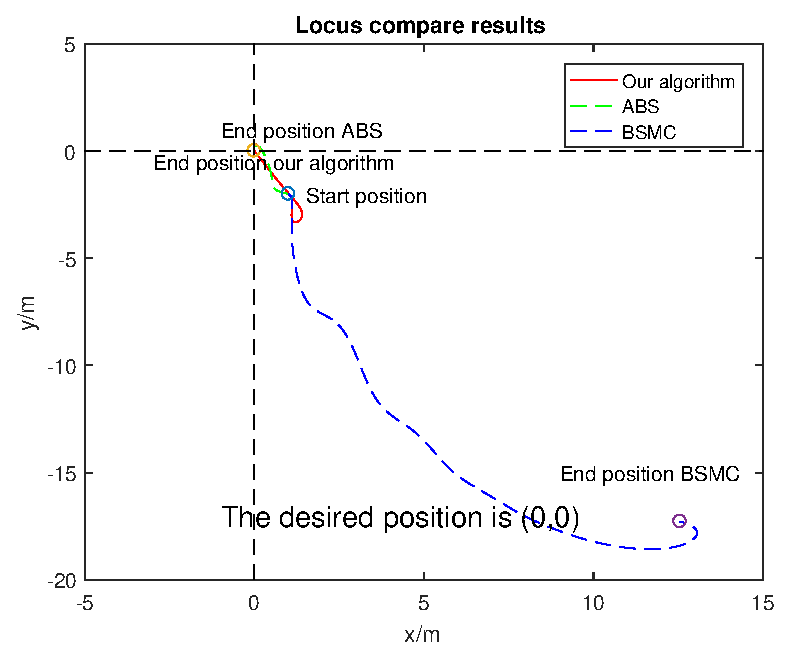
\includegraphics[width=0.45\textwidth]{figure/chap03/case0s-locus.eps}
    \hspace{1em}
    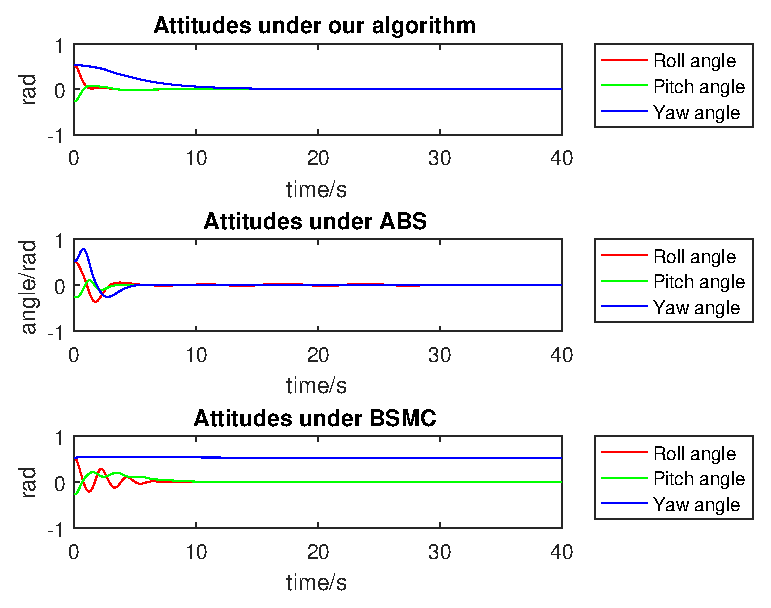
\includegraphics[width=0.45\textwidth]{figure/chap03/case0s-attitudes.eps}
    \bicaption[fig:case0s-locusandattitudes]{初始状态1轨迹图与姿态角对比}{初始状态1轨迹图与姿态角对比}{Fig.}{Trajectories and attitudes compare no disturbance: Case 1}
\end{figure}
\begin{figure}[!h]
    \centering
    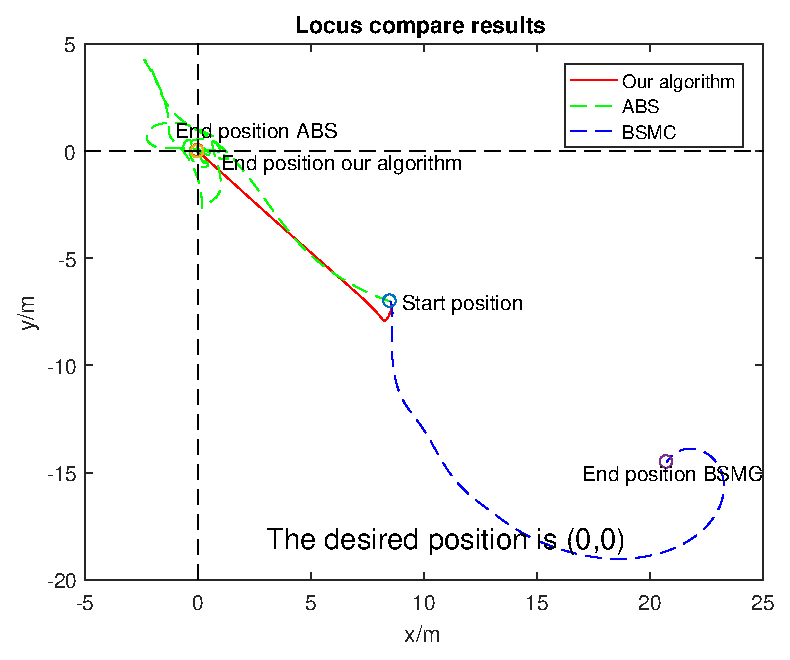
\includegraphics[width=0.45\textwidth]{figure/chap03/case0-locus.eps}
    \hspace{1em}
    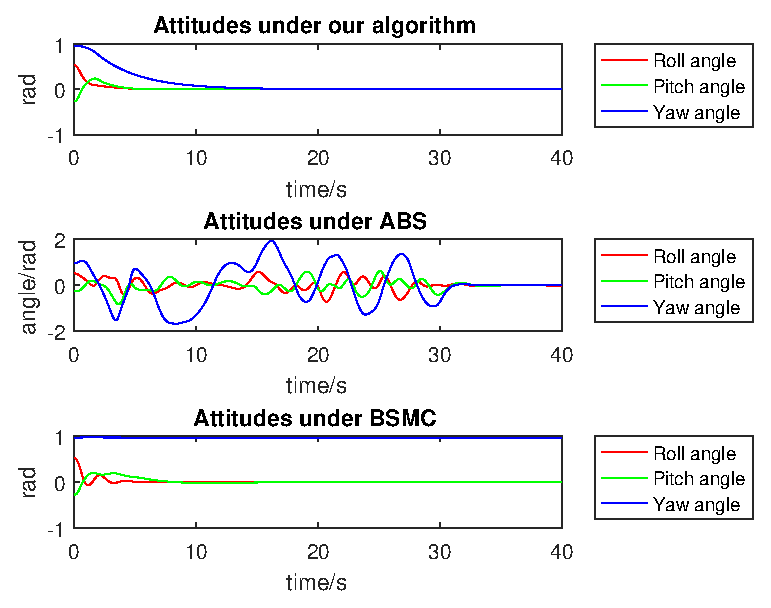
\includegraphics[width=0.45\textwidth]{figure/chap03/case0-attitudes.eps}
    \bicaption[fig:case0-locusandattitudes]{初始状态2轨迹图与姿态角对比}{初始状态2轨迹图与姿态角对比}{Fig.}{Trajectories and attitudes compare no disturbance: Case 2}
\end{figure}

图\newref{fig:case0s-locusandattitudes}与\newref{fig:case0-locusandattitudes}给出了两种初始状态下三种算法的浮空器路径、姿态角对比。从结果我们可以看出来本章\newref{sec:3algo}节的算法与文献\citen{han2015adaptive}中的算法都能很好地完成飞艇姿态稳定。文献\citen{Yang2016Positioning}的算法并不能在六自由度的情形下控制水平位置和偏航角。


\begin{comment}
\begin{figure}[!h]
    \centering
    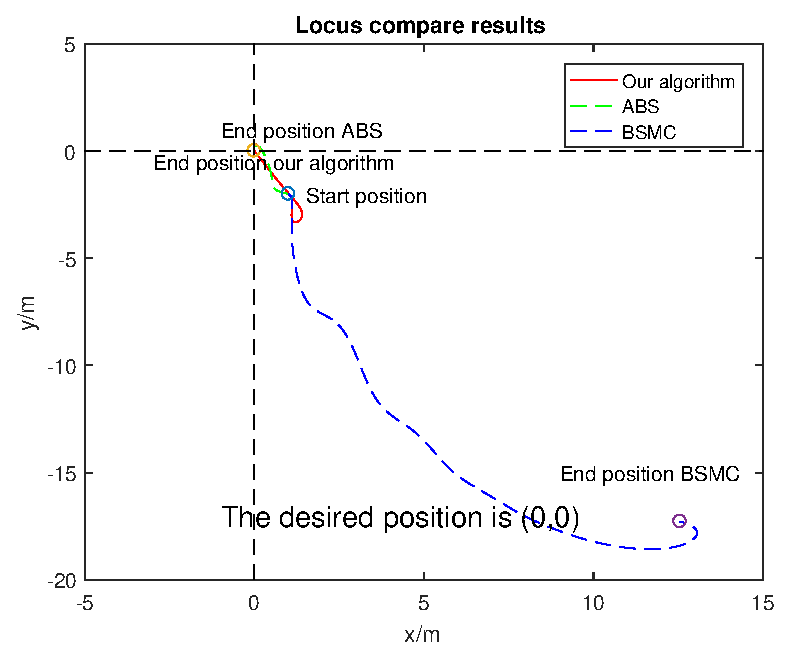
\includegraphics[width=0.7\textwidth,clip]{figure/chap03/case0s-locus.eps}
    \bicaption[fig:case0s-locus]{初始状态1轨迹图对比}{初始状态1轨迹图对比}{Fig.}{Trajectories compare with smaller initial bias and no disturbance: Case 1}
\end{figure}
\begin{figure}[!h]
    \centering
    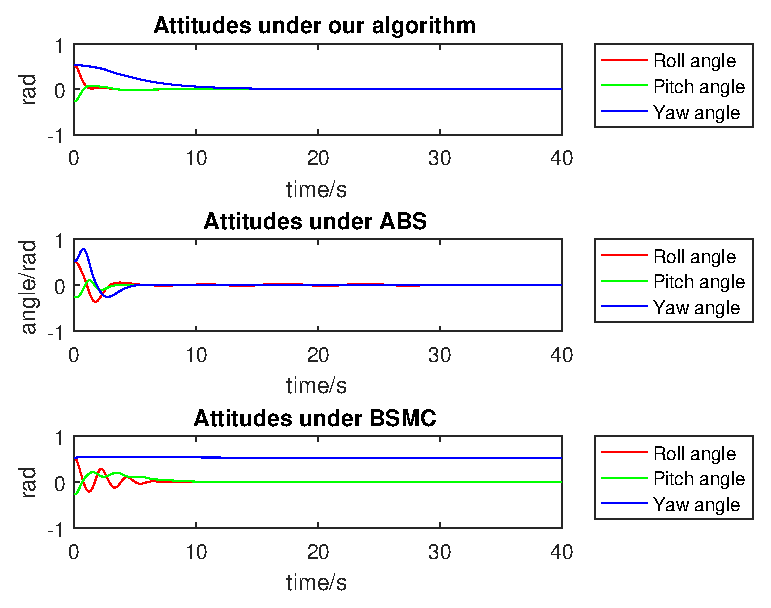
\includegraphics[width=0.8\textwidth,clip]{figure/chap03/case0s-attitudes.eps}
    \bicaption[fig:case0s-attitudes]{初始状态1姿态角对比}{初始状态1姿态角对比}{Fig.}{Attitudes with smaller initial bias and no disturbance}
\end{figure}
\begin{figure}[!h]
    \centering
    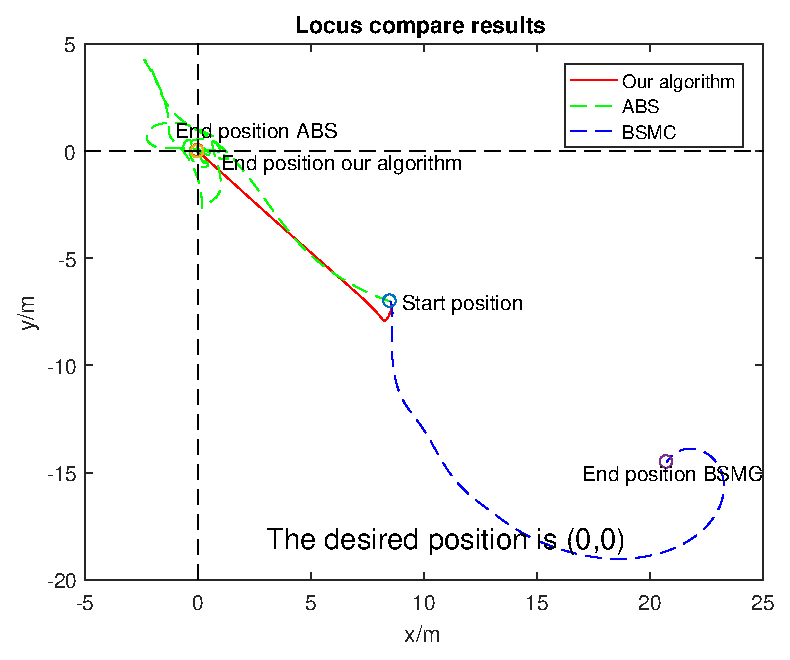
\includegraphics[width=0.45\textwidth,clip]{figure/chap03/case0-locus.eps}
    \bicaption[fig:case0-locus]{初始状态2轨迹图对比}{初始状态2轨迹图对比}{Fig.}{Trajectories compare with smaller initial bias and no disturbance: Case 2}
\end{figure}
\begin{figure}[!h]
    \centering
    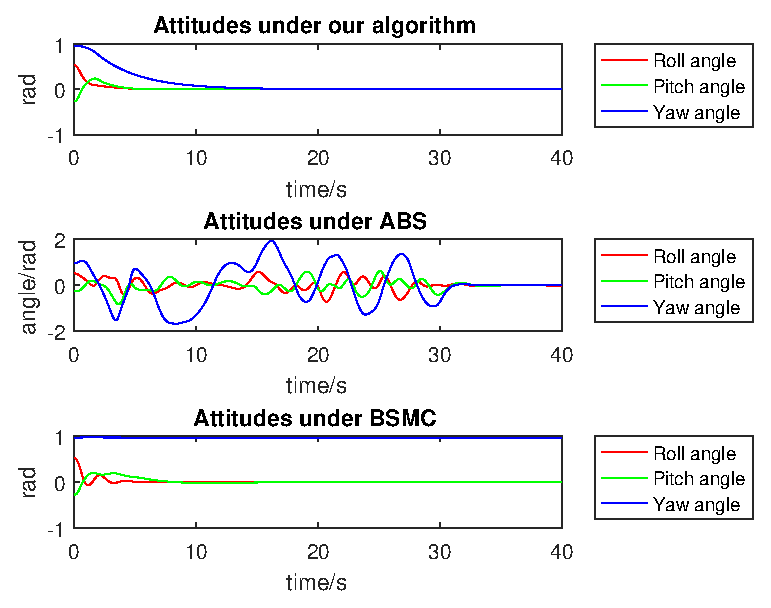
\includegraphics[width=0.45\textwidth,clip]{figure/chap03/case0-attitudes.eps}
    \bicaption[fig:case0-attitudes]{初始状态2姿态角对比}{初始状态2姿态角对比}{Fig.}{Attitudes with smaller initial bias and no disturbance: Case 2}
\end{figure}
\end{comment}

\subsection{仿真2:有扰动情况,自适应滑模抗扰动算法}\label{sec:sim3-2}
本次仿真中,浮空器的初始状态与表\newref{tab:initstate0}的相同,添加的扰动在表\newref{tab:distur1}中给出,其中$X$是服从正态分布的随机变量,满足$X\sim\mathcal{N}(0,1)$。
\begin{table}[htp]
    \centering
    \bicaption[tab:distur1]{仿真2中的扰动}{仿真2中的扰动}{Table}{The disturbances in simulation 2}
    \vspace{0.5em}
    \begin{tabular}{cl}
        \toprule
        扰动变量&扰动值  \\
        \midrule
        $m_{11}$/kg&$10.8147+10\mathrm{sin}(t)$\\
        $m_{22}$/kg&$10.8147+10\mathrm{cos}(t)$\\
        $m_{55}$/kg&$19.3024-50\mathrm{cos}(t)$\\
        $C_x$&$C_x+0.5X$\\
        \bottomrule
    \end{tabular}    
\end{table}

浮空器轨迹的仿真结果在图\newref{fig:case1-locus}中给出。姿态角、速度、角速度的对比分别在图 \ref{fig:case1-attitudes}到\ref{fig:case1-angularvelocities}中给出。 图 \ref{fig:case1-inputAS}到\ref{fig:case1-inputBSMC} 给出了不同算法的控制输入。

\begin{figure}[!htp]
    \centering
    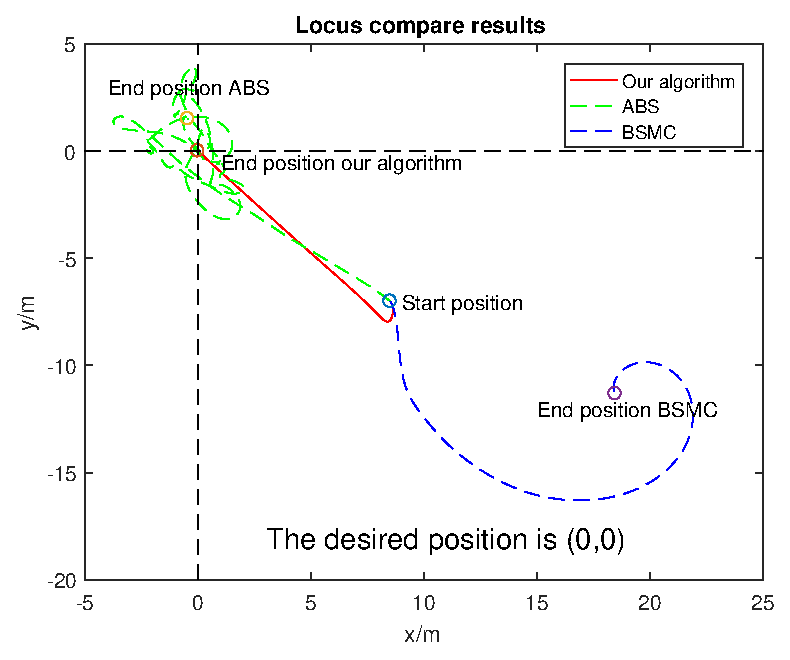
\includegraphics[width=0.7\textwidth]{figure/chap03/case1-locus.eps}
    \bicaption[fig:case1-locus]{仿真2轨迹对比}{仿真2轨迹对比}{Fig.}{Trajectories compare with disturbance under simulation 2}
\end{figure}
\begin{figure}[!htp]
    \centering
    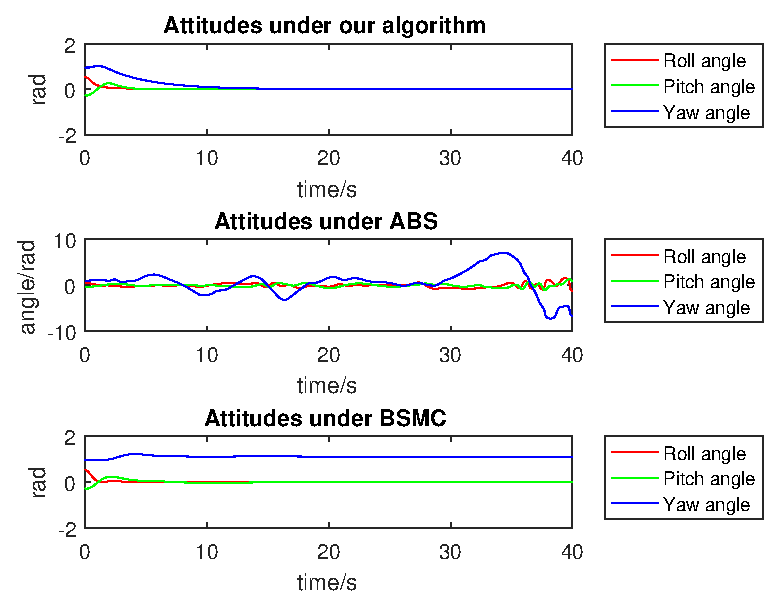
\includegraphics[width=0.7\textwidth,clip]{figure/chap03/case1-attitudes.eps}
    \bicaption[fig:case1-attitudes]{仿真2姿态角对比}{仿真2姿态角对比}{Fig.}{Attitudes compare with disturbance under simulation 2}
\end{figure}
\begin{figure}[!htp]
    \centering
    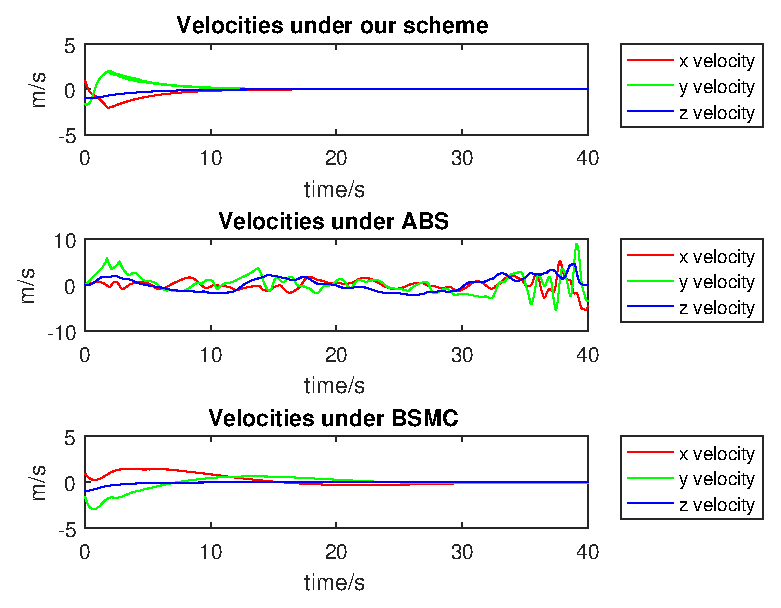
\includegraphics[width=0.7\textwidth,clip]{figure/chap03/case1-velocities.eps}
    \bicaption[fig:case1-velocities]{仿真2浮空器速度对比}{仿真2浮空器速度对比}{Fig.}{Attitudes compare with disturbance under simulation 2}
\end{figure}
\begin{figure}[!htp]
    \centering
    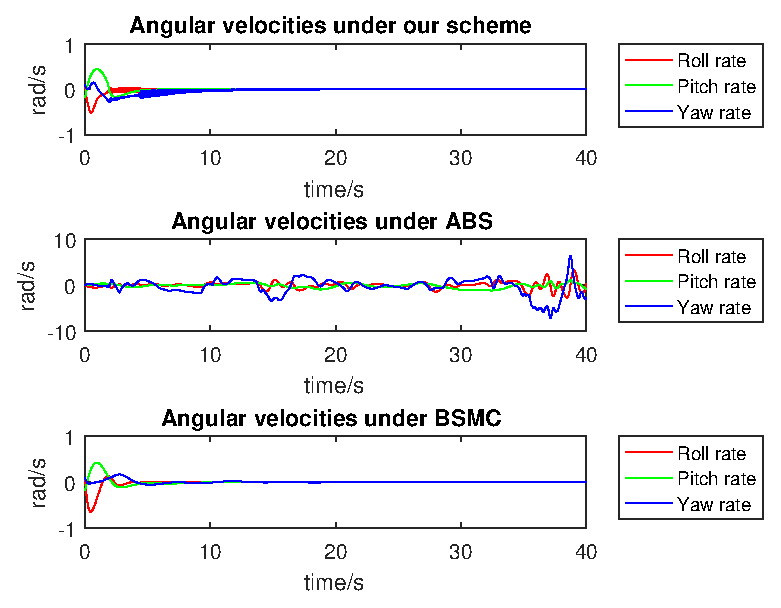
\includegraphics[width=0.7\textwidth,clip]{figure/chap03/case1-angularvelocities.eps}
    \bicaption[fig:case1-angularvelocities]{仿真2浮空器角速度对比}{仿真2浮空器角速度对比}{Fig.}{Angular velocities compare with disturbance under simulation 2}
\end{figure}
\begin{figure}[!htp]
    \centering
    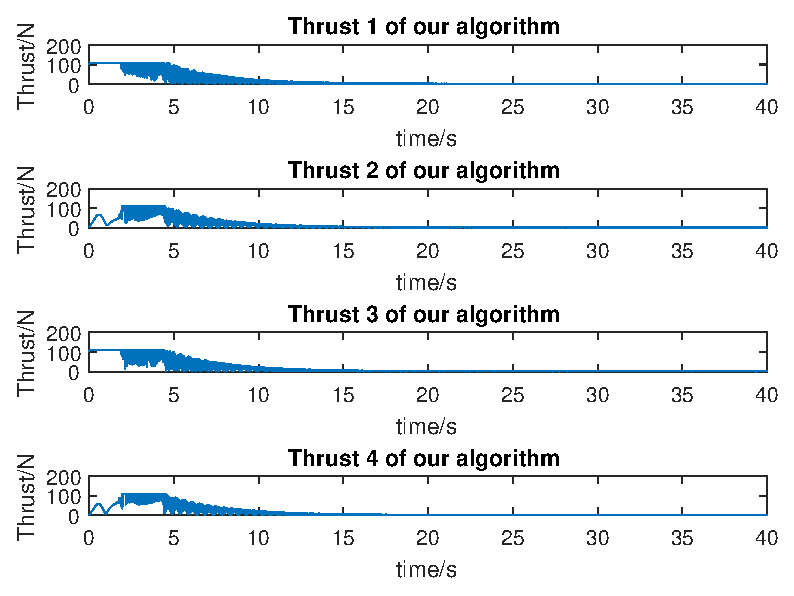
\includegraphics[width=0.7\textwidth,clip]{figure/chap03/case1-inputAS.eps}
    \bicaption[fig:case1-inputAS]{仿真2本文\newref{sec:3algo}算法执行机构输出}{仿真2本文\newref{sec:3algo}算法执行机构输出}{Fig.}{Thrust input forces of algorithm in \newref{sec:3algo} under simulation 2}
\end{figure}
\begin{figure}[!htp]
    \centering
    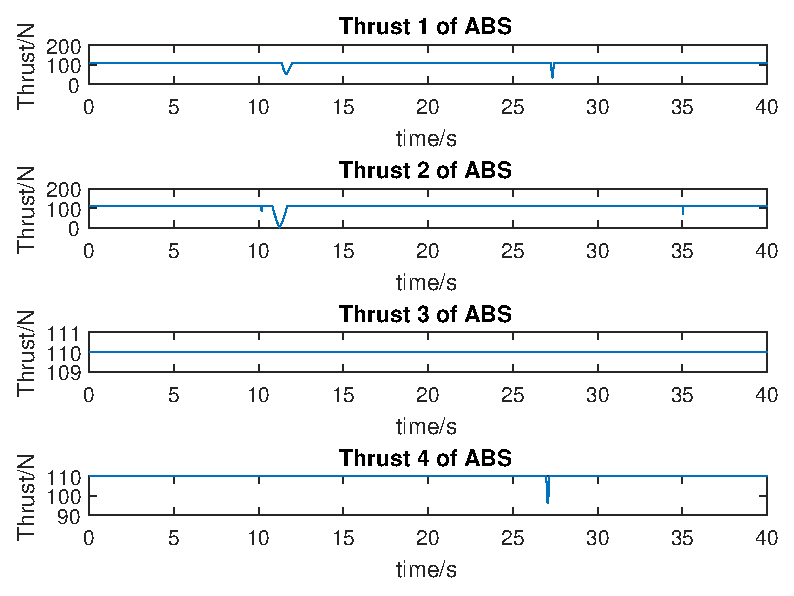
\includegraphics[width=0.7\textwidth,clip]{figure/chap03/case1-inputABS.eps}
    \bicaption[fig:case1-inputABS]{仿真2 ABS算法执行机构输出}{仿真2 ABS算法执行机构输出}{Fig.}{Thrust input forces of ABS algorithm\cite{han2015adaptive} under simulation 2}
\end{figure}
\begin{figure}[!htp]
    \centering
    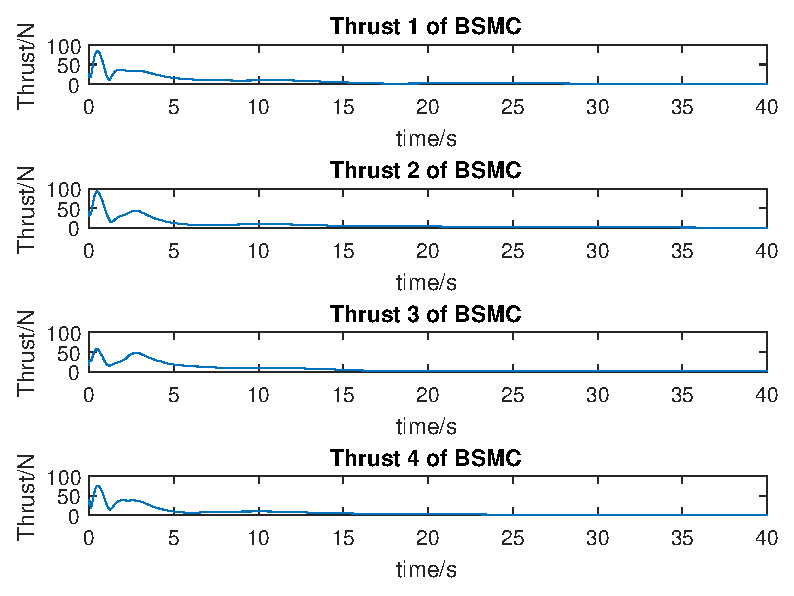
\includegraphics[width=0.6\textwidth,clip]{figure/chap03/case1-inputBSMC.eps}
    \bicaption[fig:case1-inputBSMC]{仿真2 BSMC算法执行机构输出}{仿真2 BSMC算法执行机构输出}{Fig.}{Thrust input forces of BSMC algorithm\cite{Yang2016Positioning} under simulation 2}
\end{figure}

\subsection{仿真3:有扰动,自适应滑模抗扰动考虑饱和算法}\label{sec:sim3-3}

本次仿真中,浮空器的初始状态在表\newref{tab:initstate2}中给出,添加的扰动与表\newref{tab:distur1}中相同。

\begin{table}[htp]
    \centering
    \bicaption[tab:initstate2]{仿真3初始状态}{仿真3初始状态}{Table}{The initial state of the airship under simulation 3}
    \vspace{0.5em}
    \begin{tabular}{cl}
        \toprule
        状态变量&值  \\
        \midrule
        $\mathbf{P}(m)$&$[-8.5,9,4]^T$  \\
        $\mathbf{\Omega}$(rad)&$[\pi/6,-\pi/12,\pi/3]^T$  \\
        $\mathbf{v}$(m/s)&$[1,-1.5,-1]^T$  \\
        $\mathbf{w}$(rad/s)&$[0.1,-0.2,0.1]^T$\\
        \bottomrule
    \end{tabular}    
\end{table}

\begin{figure}[!htp]
    \centering
    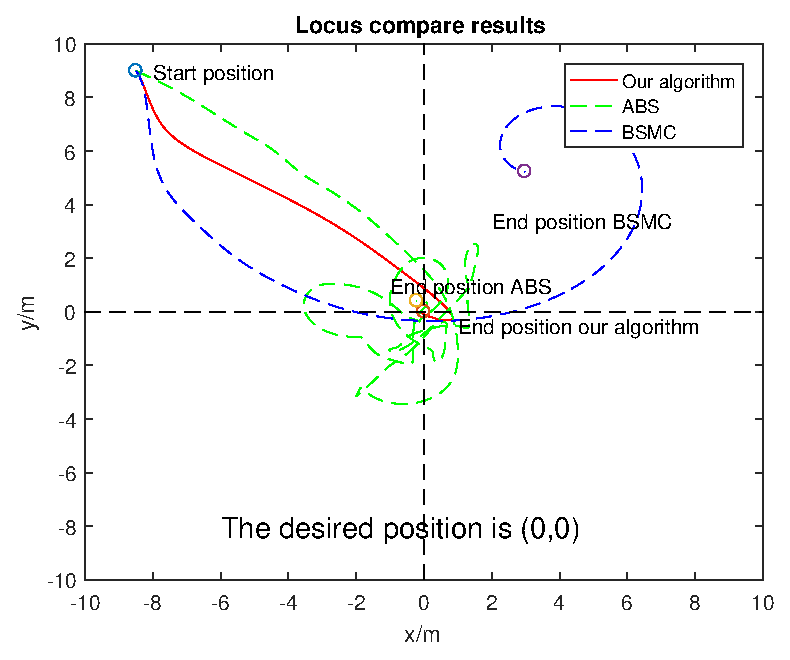
\includegraphics[width=0.7\textwidth]{figure/chap03/case2-locus.eps}
    \bicaption[fig:case2-locus]{仿真3轨迹对比}{仿真3轨迹对比}{Fig.}{Trajectories compare with disturbance under simulation 3}
\end{figure}
\begin{figure}[!htp]
    \centering
    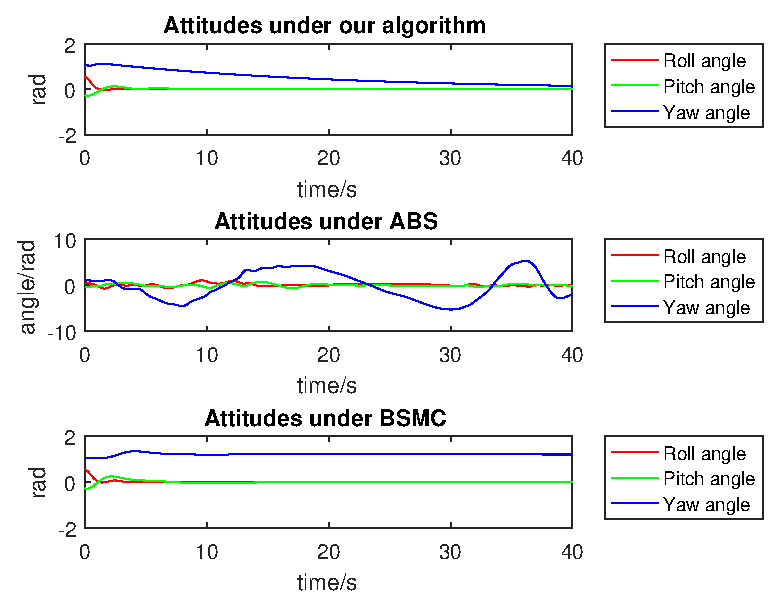
\includegraphics[width=0.7\textwidth,clip]{figure/chap03/case2-attitudes.eps}
    \bicaption[fig:case2-attitudes]{仿真3姿态角对比}{仿真3姿态角对比}{Fig.}{Attitudes compare with disturbance under simulation 3}
\end{figure}
\begin{figure}[!htp]
    \centering
    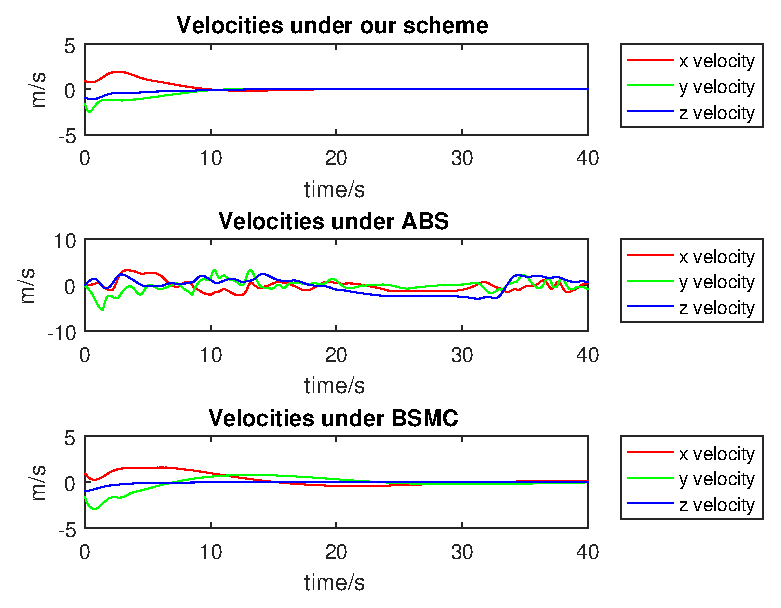
\includegraphics[width=0.7\textwidth,clip]{figure/chap03/case2-velocities.eps}
    \bicaption[fig:case2-velocities]{仿真3浮空器速度对比}{仿真3浮空器速度对比}{Fig.}{Attitudes compare with disturbance under simulation 3}
\end{figure}
\begin{figure}[!htp]
    \centering
    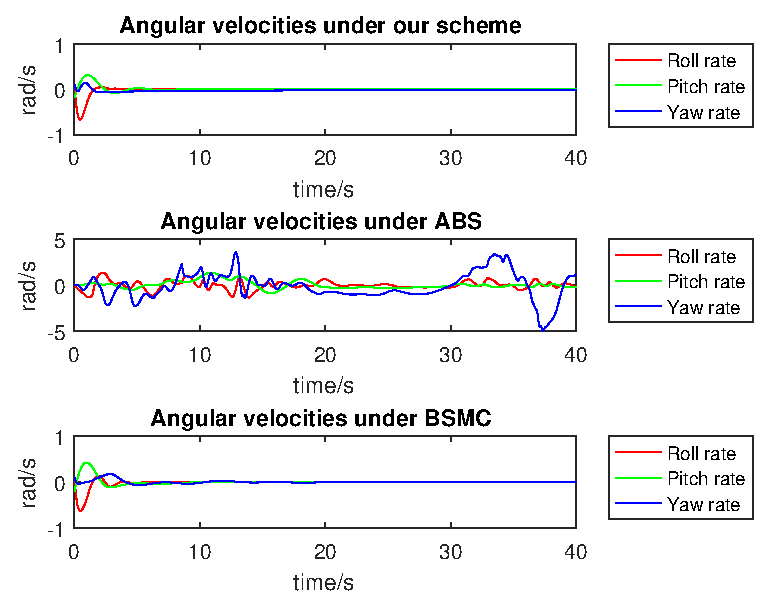
\includegraphics[width=0.7\textwidth,clip]{figure/chap03/case2-angularvelocities.eps}
    \bicaption[fig:case2-angularvelocities]{仿真3浮空器角速度对比}{仿真3浮空器角速度对比}{Fig.}{Angular velocities compare with disturbance under simulation 3}
\end{figure}
\begin{figure}[!htp]
    \centering
    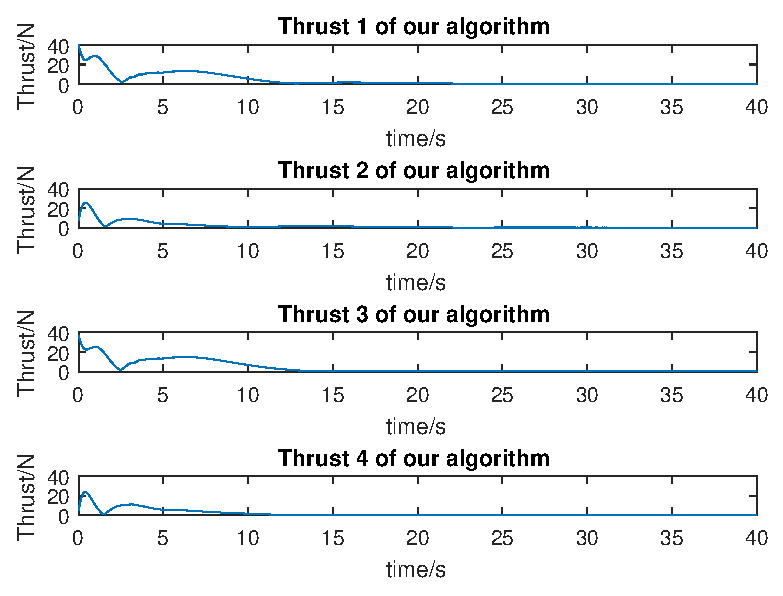
\includegraphics[width=0.7\textwidth,clip]{figure/chap03/case2-inputAS.eps}
    \bicaption[fig:case2-inputAS]{仿真3本文\newref{sec:3algo}算法执行机构输出}{仿真3本文\newref{sec:3algo}算法执行机构输出}{Fig.}{Thrust input forces of algorithm in \newref{sec:3algo} under simulation 3}
\end{figure}
\begin{figure}[!htp]
    \centering
    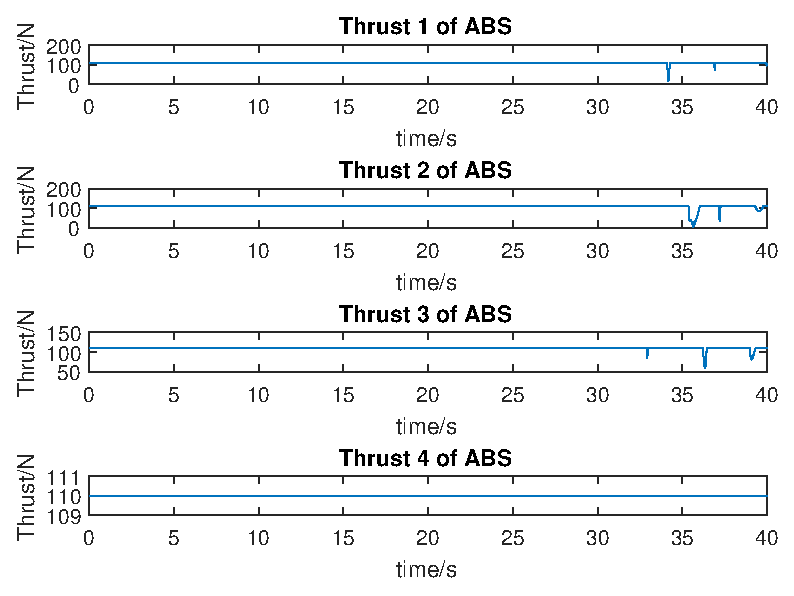
\includegraphics[width=0.7\textwidth,clip]{figure/chap03/case2-inputABS.eps}
    \bicaption[fig:case2-inputABS]{仿真3 ABS算法执行机构输出}{仿真3 ABS算法执行机构输出}{Fig.}{Thrust input forces of ABS algorithm\cite{han2015adaptive} under simulation 3}
\end{figure}
\begin{figure}[!htp]
    \centering
    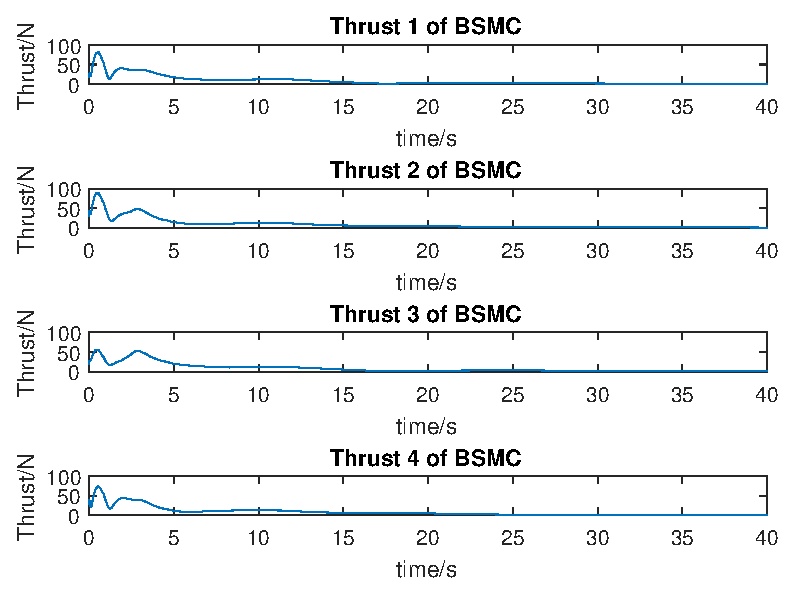
\includegraphics[width=0.6\textwidth,clip]{figure/chap03/case2-inputBSMC.eps}
    \bicaption[fig:case2-inputBSMC]{仿真3 BSMC算法执行机构输出}{仿真3 BSMC算法执行机构输出}{Fig.}{Thrust input forces of BSMC algorithm\cite{Yang2016Positioning} under simulation 3}
\end{figure}

从仿真2和仿真3中,我们可以观察到:
\begin{enumerate}
    \item D.Han的自适应反演算法与浮空器的初始状态高度相关,如果初始状态偏移过大,其算法会剧烈振荡。注意到在D.Han的算法中其执行机构一直在满负荷状态附近工作,这说明其算法虽然具有鲁棒性,但是并不稳定。
    \item 从图\newref{fig:case0s-locusandattitudes}、\newref{fig:case0-locusandattitudes}、\newref{fig:case1-attitudes}和\newref{fig:case2-attitudes}可以看出,Y.Yang的针对三自由度模型的反演滑模算法在处理六自由度模型的时候并不适用。
    \item 本文\newref{sec:3algo}节提出的算法可以很好地处理不不确定性带来的影响,曲线较为平滑,但从图\newref{fig:case1-inputAS}可以看出,其缺陷是执行机构抖震过于明显,且前期输出一直在满负荷附近。但是在\newref{sec:3sat}节的抗饱和算法的结果中(图\newref{fig:case2-inputAS}),执行机构的输出幅度得到了明显的下降,这说明\newref{sec:3sat}提出的抗饱和算法是有效的。
\end{enumerate}

\subsection{仿真4:大偏移长时间仿真}\label{sec:sim3-4}
由于本文提出的自适应滑模算法在系统稳定前会导致估测参数的持续增加,而仿真1至仿真3中采用的都是较小初始偏移量,所以在此增加一例大偏移仿真,以观察系统的收敛时间以及自适应参数增加情况。本次仿真系统的初始状态如表\newref{tab:initstate3}所示,添加扰动与表\newref{tab:distur1}中相同,本次仿真仅采用\newref{sec:3sat}节中的算法,未作对比。

\begin{table}[htp]
    \centering
    \bicaption[tab:initstate3]{仿真4初始状态}{仿真4初始状态}{Table}{The initial state of the airship under simulation 4}
    \vspace{0.5em}
    \begin{tabular}{cl}
        \toprule
        状态变量&值  \\
        \midrule
        $\mathbf{P}(m)$&$[500,500,100]^T$  \\
        $\mathbf{\Omega}$(rad)&$[\pi/4,-\pi/3,\pi/3]^T$  \\
        $\mathbf{v}$(m/s)&$[8,-10,-8]^T$  \\
        $\mathbf{w}$(rad/s)&$[0.3,-0.4,0.3]^T$\\
        \bottomrule
    \end{tabular}    
\end{table}

\begin{figure}[!htp]
    \centering
    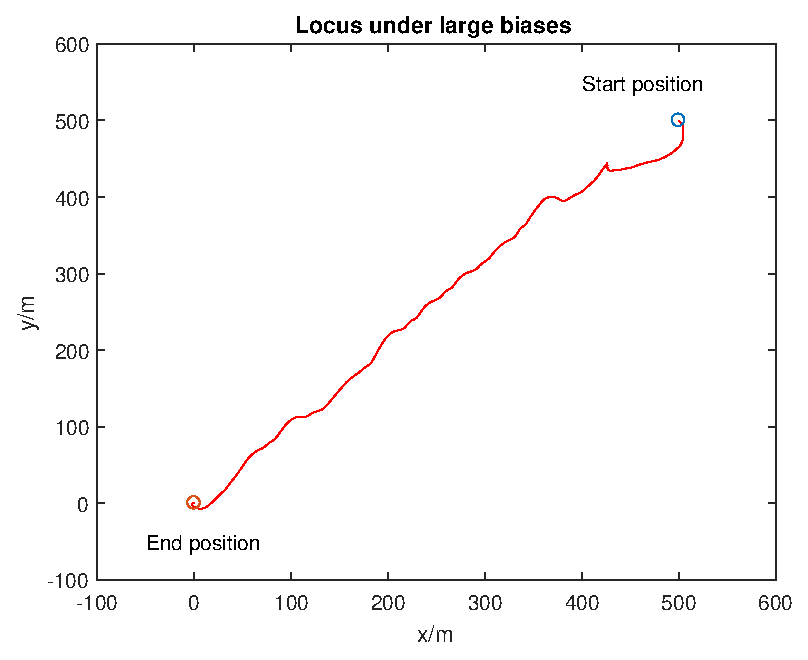
\includegraphics[width=0.7\textwidth]{figure/chap03/case3-locus.eps}
    \bicaption[fig:case3-locus]{仿真4轨迹对比}{仿真4轨迹对比}{Fig.}{Trajectories under simulation 4}
\end{figure}
\begin{figure}[!htp]
    \centering
    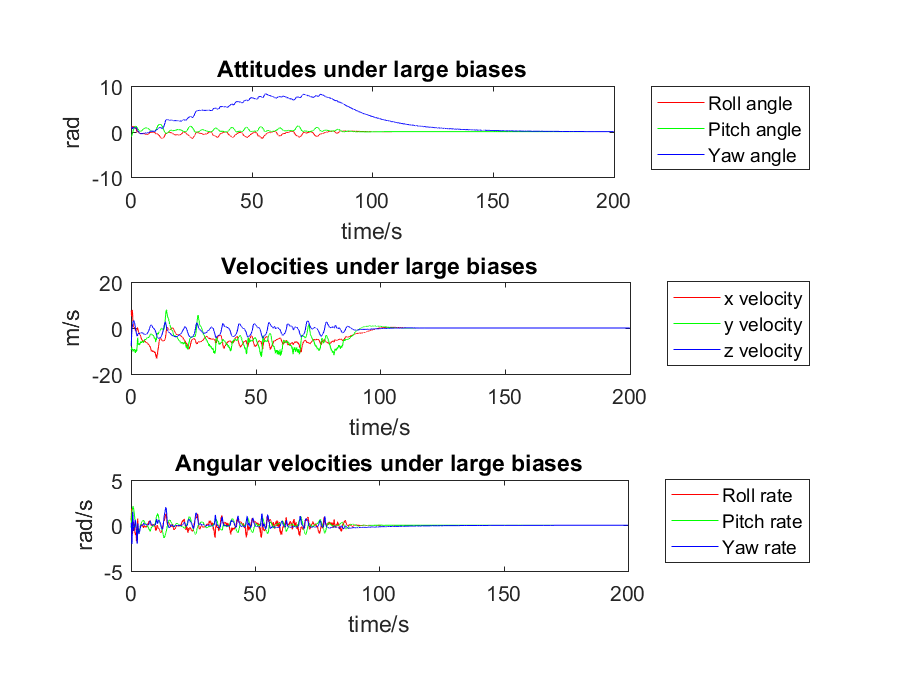
\includegraphics[width=0.7\textwidth,clip]{figure/chap03/case3-states.eps}
    \bicaption[fig:case3-states]{仿真4浮空器各状态}{仿真4浮空器各状态}{Fig.}{Airship states under simulation 4}
\end{figure}
\begin{figure}[!htp]
    \centering
    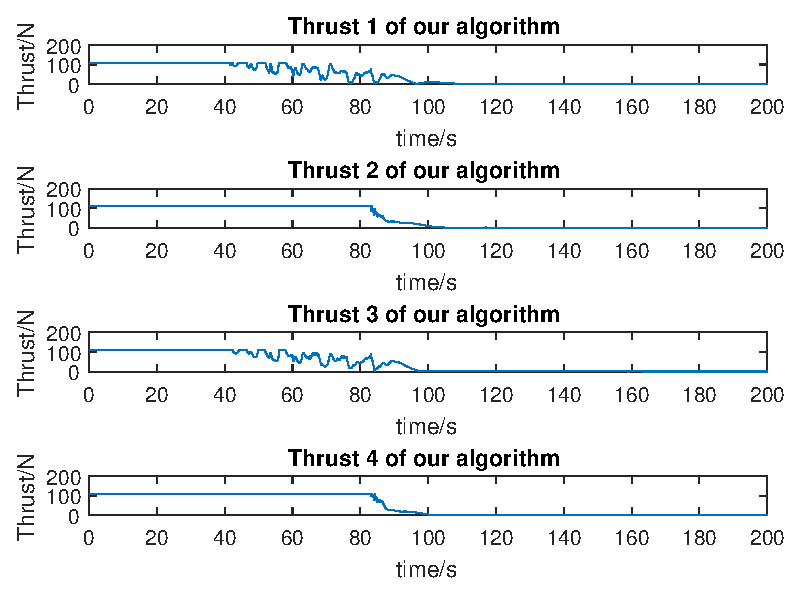
\includegraphics[width=0.7\textwidth,clip]{figure/chap03/case3-inputAS.eps}
    \bicaption[fig:case3-inputAS]{仿真4浮空器执行机构输出大小}{仿真4浮空器执行机构输出大小}{Fig.}{Thrust input forces under simulation 4}
\end{figure}
\begin{figure}[!htp]
    \centering
    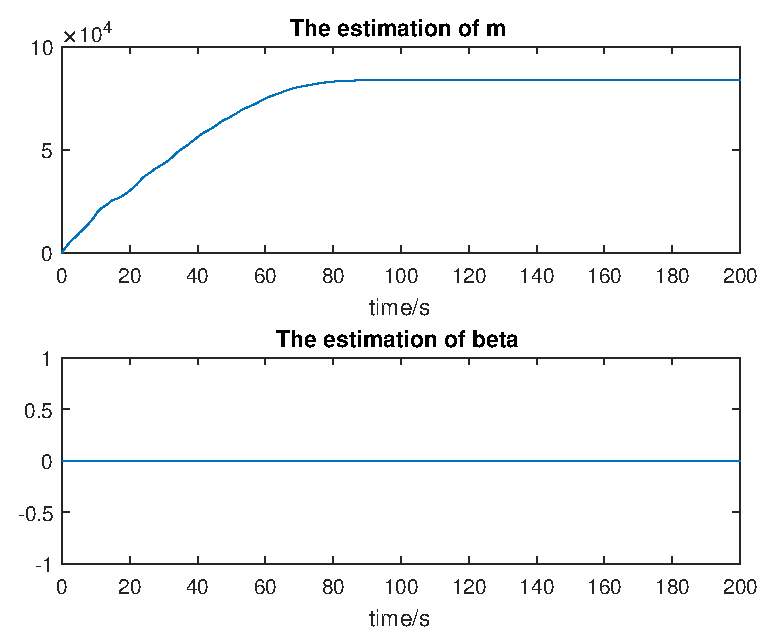
\includegraphics[width=0.7\textwidth,clip]{figure/chap03/case3-paraest.eps}
    \bicaption[fig:case3-paraest]{仿真4自适应参数估计}{仿真4自适应参数估计}{Fig.}{Adaptive parameters estimations under simulation 4}
\end{figure}

从图\newref{fig:case3-locus}至\newref{fig:case3-states}可以看出浮空器大约在90秒的时候回到预定地点保持稳定。图\newref{fig:case3-paraest}说明参数$\hat{\beta}$是稳定的,$\hat{m}$在系统尚未到达滑模面之前是急剧增加的,但在系统接近稳定点的时候就趋于平滑。调节参数$p_3$与$p_4$的值可以减缓这个步骤,但是并不能消除参数无限制增加的影响,这也是本算法的一个缺陷,需要在后续研究中加以克服。


\section{本章小结}
本章介绍了一种基于自适应滑模方法的抗参数扰动的容错控制策略,并在提出算法的基础上添加了抗饱和机制。浮空器特有的高附加质量和气动参数不准确问题,给它的稳定控制增加了很大的困难。本章\newref{sec:3algo}节的算法能够在浮空器同时遭到惯性矩阵扰动和气动参数扰动的前提下使其保持稳定;而\newref{sec:3sat}节提出的算法则对\newref{sec:3algo}节的算法进行了改进,添加了抗饱和机制。为了说明算法的有效性,本章在四种情形下分别对算法做了数值仿真,并且与已有的浮空器鲁棒控制算法进行了对比。
%# -*- coding: utf-8-unix -*-
%%==================================================
%% chapter01.tex for SJTU Master Thesis
%%==================================================

%\bibliographystyle{sjtu2}%[此处用于每章都生产参考文献]
\chapter{一种基于自适应积分滑模方法的抗参数扰动与执行机构故障的控制策略}
\label{chap:aismc}
\section{引言}
第\ref{chap:asmcsat}章介绍了一种能应对惯性矩阵扰动和气动系数扰动的自适应滑模算法。但是没有考虑执行机构故障。然而执行机构故障对于平流层浮空器来说是一种常见的故障,应当被考虑在内。其实,第\ref{chap:asmcsat}章的算法可以稍做修改,就能处理执行机构不确定的问题。比如把不确定的执行机构函数加入假设\newref{3ass:F}和\newref{3ass:MCJ}中。但是这样的做法将所有不确定性都同时处理了,并不能根据执行机构的错误严重程度进行参数调节。此外,第\ref{chap:asmcsat}章的算法只能定点稳定浮空器,但有时执行任务时浮空器需要在多个任务地点之间往返。本章通过引入积分滑模面,重新设计了一个自适应积分滑模控制器,解决了处理执行机构故障的问题,提出了一个能够同时处理惯性矩阵不确定、气动系数不确定、外部扰动、执行机构效率矩阵不确定以及执行机构输出有偏移情况的浮空器位置追踪算法。本节算法的特色是提出的控制算法中每种错误都对应一个调节参数,以应对不同等级的不确定性。

本文已经在第\ref{chap:preliminary}章给出了执行机构的故障建模,这里稍作回顾。

螺旋桨遇到的问题可以归结为效率损失、输出偏移,卡顿和失效等几类。假设某个执行机构$i$的期望输出为$\upsilon_i$, 其输出效率为$\varepsilon_i$,输出偏移为$\bar{\upsilon_i}$,那么式\newref{eq:outputeff}给出了它们之间的关系:
\begin{equation*}
    u_{ai} = \varepsilon_i(t)\upsilon_i+\bar{\upsilon_i}
\end{equation*}

对于上述提到的各种故障,可总结其数学模型于表\newref{tab:faultmodelc4}。
\begin{table}[ht]
    \centering
	\bicaption[tab:faultmodelc4]{螺旋桨故障及其数学模型}{螺旋桨故障及其数学模型}{Table}{Thrust fault classifications and math models}
	\vspace{0.5em}
	\begin{tabular}{lll}
		\toprule
		故障类型&$\varepsilon_i(t)$&$\bar{\upsilon}_i$ \\
		\midrule
		正常&$\varepsilon_i(t)=1$&$\bar{\upsilon}_i=0$\\
		效率损失&$\varepsilon_i(t)<1$&$\bar{\upsilon}_i=0$\\
		输出偏移&$\varepsilon_i(t)=1$&$\bar{\upsilon}_i\neq0$\\
		卡顿&$\varepsilon_i(t)=0$&$\upsilon_i\neq0$\\
		失效&$\varepsilon_i(t)=0$&$\upsilon_i=0$\\
		\bottomrule
	\end{tabular}
\end{table}

浮空器的实际输出$\mathbf{F_t}$可用式\neweqref{eq:inputtransc4}表示

\begin{equation}\label{eq:inputtransc4}
    \mathbf{F_t} = \mathbf{Du_a} = \mathbf{D}[EF_{HV} + \bar{\upsilon}]
\end{equation}

其中$\mathbf{D}$在式\neweqref{eq:D}中给出,其他参数

\begin{equation*}
    E = \left[\begin{matrix}
    \varepsilon_1&&&&&&&\\
    &\varepsilon_2&&&&&&\\
    &&\varepsilon_3&&&&&\\
    &&&\varepsilon_4&&&&\\
    &&&&\varepsilon_5&&&\\
    &&&&&\varepsilon_6&&\\
    &&&&&&\varepsilon_7&\\
    &&&&&&&\varepsilon_8\\
    \end{matrix}\right]
\end{equation*}

\begin{equation*}
    \bar{\upsilon} = \left[\begin{matrix}
    \bar{\upsilon}_1&\bar{\upsilon}_2&\cdots&\bar{\upsilon}_8
    \end{matrix}\right]^T
\end{equation*}
$E$为执行机构效率矩阵,$\bar{\upsilon}$为执行机构输出偏移向量。$F_{HV}$则是浮空器实际执行机构输入的非线性函数。

\section{问题描述}
在提出故障模型后,浮空器的不确定模型为
\begin{equation}\label{eq:4uncertainmodel}
    \begin{cases}
    \hspace{1em}\dot{\mathbf{x}}_1 &= \mathbf{J}\mathbf{x}_2\\
    \mathbf{M}\dot{\mathbf{x}}_2&=\mathbf{F_{gb}+F_{i}(x_2)}+\mathbf{S(x_2)}\mathbf{c}+\mathbf{D}[EF_{HV} + \bar{\upsilon}]+\mathbf{d}
    \end{cases}
\end{equation}

其中$\mathbf{M}$、$\mathbf{c}$、$\bar{\upsilon}$、$\mathbf{d}$均未知。本节目的是对模型\newref{eq:4uncertainmodel}设计一个控制器,使得浮空器能跟踪所给位置和姿态角信号并保持稳定。

\section{算法详述}

为了引入算法,首先引入如下合理的假设

\begin{ass}\label{4ass}
    假定浮空器的几个不确定参数的模都小于某个未知的上界,即
    \begin{eqnarray}
    \bnorm{M} &\leqslant M_{max} \\
    \bnorm{c} &\leqslant c_{max} \\
    \bnorm{d} &\leqslant d_{max} \\
    \bar{\upsilon} &\leqslant \bar{\upsilon}_{max} \\
    \end{eqnarray}
\end{ass}

本章的目的在假设\newref{4ass}的前提下,为模型\newref{eq:4uncertainmodel}是设计一个能跟踪位置和姿态角信号的控制器。首先引入跟踪误差$\mathbf{e}(t)$:
\begin{equation}\label{eq:errordef}
    \mathbf{e}(t)=\mathbf{J}^{-1}(\mathbf{x}_1-\mathbf{x}_{1d})
\end{equation}

其中$\mathbf{x}_{1d}$表示要追踪的信号。

引入积分滑模面
\begin{equation}\label{eq:slidingsurface}
\mathbf{s}(t)=\dot{\mathbf{e}}(t)-\dot{\mathbf{e}}(0)-\int_{0}^{t}[-\alpha\dot{\mathbf{e}}(\tau)-\beta\mathbf{e}(\tau)]\mathrm{d}\tau
\end{equation}

其中 $\alpha,\beta>0$是可选标量参数。根据滑模理论,当系统轨迹达到滑模面时,有$\dot{\mathbf{s}}=\mathbf{s}=0$,即

\begin{equation}
    \ddot{\mathbf{e}}(t)+\alpha\dot{\mathbf{e}}(t)+\beta\mathbf{e}=0
\end{equation}

选取$\alpha$和$\beta$使方程$x^2+\alpha x+\beta=0$有两个负实根,则当$\mathbf{s}(t)=0$时,$\mathbf{e}(t)$会渐进收敛到原点。

沿袭第\ref{chap:asmcsat}章自适应滑模控制器的设计思路,本章给传统的滑模面添加一个积分项,用以减小系统到达滑模面的时间。

基于滑模面\neweqref{eq:slidingsurface}和假设\newref{4ass},提出如下控制器:
\begin{align}\label{eq:4controller}
\upsilon=&-\frac{\bnorm{F}\mathbf{D}^T\mathbf{s}(t)}{\sigma \snorm}
-\frac{\bnorm{D}\hat{\bar{\upsilon}}_{max}\mathbf{D}^T\mathbf{s}(t)}{k_1 \snorm}
-\frac{\bnorm{S}\hat{c}_{max}\mathbf{D}^T\mathbf{s}(t)}{k_2 \snorm} \nonumber
\\&-\frac{\hat{d}_{max}\mathbf{D}^T\mathbf{s}(t)}{k_3 \snorm}-\frac{\bnorm{G}\hat{M}_{max}\mathbf{D}^T\mathbf{s}(t)}{k_4 \snorm}
-\frac{\mu\mathbf{D}^T\mathbf{s}(t)}{\snorm}
\end{align}

其中$k_1,\quad k_2,\quad k_3,\quad k_4>0$为可选参数,且
\begin{align}
\mathbf{G} =& \mathbf{\ddot{J}^{-1}}(\mathbf{x}_1-\mathbf{x}_{1d})+\mathbf{\dot{J}^{-1}JV}+\alpha\mathbf{\dot{J}^{-1}}(\mathbf{x}_1-\mathbf{x}_{1d})
\nonumber\\&+\alpha\mathbf{V}+\beta\mathbf{J^{-1}}(\mathbf{x}_1-\mathbf{x}_{1d})
\end{align}
\begin{eqnarray}
\dot{\hat{\bar{\upsilon}}}_{max} &= -\lambda_1^2\hat{\bar{\upsilon}}_{max}+\xi_1\bnorm{D}\bnorm{s(t)} \label{eq:vupdt} \\
\dot{\hat{c}}_{max} &= -\lambda_2^2\hat{c}_{max}+\xi_2\bnorm{D}\bnorm{s(t)} \label{eq:cupdt} \\
\dot{\hat{d}}_{max} &= -\lambda_3^2\hat{d}_{max}+\xi_3\bnorm{D}\bnorm{s(t)} \label{eq:dupdt} \\
\dot{\hat{M}}_{max} &= -\lambda_4^2\hat{M}_{max}+\xi_4\bnorm{D}\bnorm{s(t)} \label{eq:Mupdt} \\
\dot{\lambda}_i&=-\kappa_i\lambda_i,\quad (i=1,2,3,4) \label{eq:lbdupdt}
\end{eqnarray}

其中$\hat{\bar{\upsilon}}_{max}$、$\hat{c}_{max}$、$\hat{d}_{max}$、$\hat{M}_{max}$可分别看做是执行机构偏移量、气动系数向量、外部扰动和惯性矩阵的上限估计值,且满足
\begin{eqnarray}
\hat{\bar{\upsilon}}_{max}(0)>0 \nonumber\\
\hat{c}_{max}(0)>0 \nonumber\\
\hat{d}_{max}(0)>0 \nonumber\\
\hat{M}_{max}(0)>0 \nonumber
\end{eqnarray}

$\xi_i,\kappa_i,\lambda_i,k_i$ 和 $\mu$ 都是正标量。 $\sigma>0$ 且满足
\begin{equation}\label{eq:sigma<dedt}
    0<\sigma<\mathbf{DE(t)D^T}
\end{equation}

注意$\mathbf{DE(t)D^T}$是一个$6\times 6$的矩阵,式\neweqref{eq:sigma<dedt}的意思是$\sigma>0$,但是小于矩阵$\mathbf{DE(t)D^T}$的最小特征值。

下面证明浮空器系统\newref{eq:4uncertainmodel}在控制器\newref{eq:4controller}的作用下,是全局渐进稳定的。取李雅普诺夫函数
\begin{align*}\label{eq:4lypa}
	V(t) =& \frac{1}{2}\mathbf{s}^T(t)\mathbf{M}\mathbf{s}(t)
	+\frac{k_1(\bar{\upsilon}_{max}-\frac{\sigma}{k_1}\hat{\bar{\upsilon}}_{max})^2}{2\sigma\xi_1}+\frac{\kappa^{-1}_1\lambda_1^2 k_1\bar{\upsilon}_{max}^2}{8\sigma\xi_1}
	\\&+\frac{k_2(c_{max}-\frac{\sigma}{k_2}\hat{c}_{max})^2}{2\sigma\xi_2}+\frac{\kappa^{-1}_2\lambda_2^2 k_2 c_{max}^2}{8\sigma\xi_2}
	+\frac{k_3(d_{max}-\frac{\sigma}{k_3}\hat{d}_{max})^2}{2\sigma\xi_3} 
	\\&+\frac{\kappa^{-1}_3\lambda_3^2 k_1 d_{max}^2}{8\sigma\xi_3}
	+\frac{k_4(M_{max}-\frac{\sigma}{k_4}\hat{M}_{max})^2}{2\sigma\xi_4}+\frac{\kappa^{-1}_4\lambda_4^2 k_4 M_{max}^2}{8\sigma\xi_4} \numberthis
\end{align*}

由于$\frac{1}{2}\mathbf{s}^T(t)\mathbf{M}\mathbf{s}(t)>0$,于是有$V>0$。

对$V$求导,可得
%\begin{align}
% \dot{V}&=\mathbf{s}^T\left[\mathbf{D}\mathbf{E}\upsilon+\mathbf{D}\mathbf{\bar{\upsilon}}+\mathbf{M}\ddot{\mathbf{J}}^{-1}(\mathbf{x}_1-\mathbf{x}_{1d})+\mathbf{M}\dot{\mathbf{J}}^{-1}\mathbf{JV}   \right]
%\end{align}
\begin{align}
	\dot{V}(t)&=\mathbf{s}^T(t)\big[\mathbf{D}\mathbf{E}(t)\upsilon+\mathbf{D}\bar{\upsilon}+\mathbf{M}\mathbf{\ddot{\mathbf{J}}}^{-1}(\mathbf{x}_1-\mathbf{x}_{1d})+\mathbf{M}\dot{\mathbf{J}}^{-1}\mathbf{JV} \nonumber
	\\&+\mathbf{F+Sc+d}+\alpha\mathbf{M}\dot{\mathbf{J}}^{-1}(\mathbf{x}_1-\mathbf{x}_{1d})+\alpha\mathbf{MV} \nonumber
	\\&+\beta\mathbf{MJ}^{-1}(\mathbf{x}_1-\mathbf{x}_{1d})\big]-\frac{(\bar{\upsilon}_{max}-\frac{\sigma}{k_1}\hat{\bar{\upsilon}}_{max})\dot{\hat{\bar{\upsilon}}}_{max}}{\xi_1} \nonumber
	\\&+\frac{\kappa_1^{-1}\lambda_1\dot{\lambda}_1k_1\bar{\upsilon}_{max}^2}{4\sigma\xi_1}	-\frac{(c_{max}-\frac{\sigma}{k_2}\hat{c}_{max})\dot{\hat{c}}_{max}}{\xi_2} \nonumber
	\\&+\frac{\kappa_2^{-1}\lambda_2\dot{\lambda}_2k_2c_{max}^2}{4\sigma\xi_2}
	-\frac{(d_{max}-\frac{\sigma}{k_3}\hat{d}_{max})\dot{\hat{d}}_{max}}{\xi_3} \nonumber
	\\&+\frac{\kappa_3^{-1}\lambda_3\dot{\lambda}_3k_3d_{max}^2}{4\sigma\xi_3}
	-\frac{(M_{max}-\frac{\sigma}{k_4}\hat{M}_{max})\dot{\hat{M}}_{max}}{\xi_4} \nonumber
	\\&+\frac{\kappa_4^{-1}\lambda_4\dot{\lambda}_4k_4M_{max}^2}{4\sigma\xi_4} \nonumber
	\\&\leqslant\mathbf{s}^T(t)\mathbf{D}\mathbf{E}(t)\mathbf{\upsilon}+\bar{v}_{max}\bnorm{D}\snorm \nonumber
	\\&+M_{max}\bnorm{G}\snorm
	+\bnorm{F}\snorm \nonumber
	\\&+c_{max}\bnorm{S}\snorm+d_{max}\snorm \nonumber
	\\&-\frac{(\bar{\upsilon}_{max}-\frac{\sigma}{k_1}\hat{\bar{\upsilon}}_{max})\dot{\hat{\bar{\upsilon}}}_{max}}{\xi_1}
	+\frac{\kappa_1^{-1}\lambda_1\dot{\lambda}_1k_1\bar{\upsilon}_{max}^2}{4\sigma\xi_1} \nonumber
	\\&-\frac{(c_{max}-\frac{\sigma}{k_2}\hat{c}_{max})\dot{\hat{c}}_{max}}{\xi_2}
	+\frac{\kappa_2^{-1}\lambda_2\dot{\lambda}_2k_2c_{max}^2}{4\sigma\xi_2} \nonumber
	\\&-\frac{(d_{max}-\frac{\sigma}{k_3}\hat{d}_{max})\dot{\hat{d}}_{max}}{\xi_3}
	+\frac{\kappa_3^{-1}\lambda_3\dot{\lambda}_3k_3d_{max}^2}{4\sigma\xi_3} \nonumber
	\\&-\frac{(M_{max}-\frac{\sigma}{k_4}\hat{M}_{max})\dot{\hat{M}}_{max}}{\xi_4}
	+\frac{\kappa_4^{-1}\lambda_4\dot{\lambda}_4k_4M_{max}^2}{4\sigma\xi_4}  \label{eq:mediumprocedure}
\end{align}

把\neweqref{eq:4controller}代入\neweqref{eq:mediumprocedure},可得
\begin{align*}
\dot{V}(t)&\leqslant-\mathbf{s}^T(t)\mathbf{DE}(t)\bigg[\frac{\bnorm{F}\mathbf{D}^T\mathbf{s}(t)}{\sigma\snorm}+\frac{\bnorm{D}\hat{\bar{\upsilon}}_{max}\mathbf{D}^T\mathbf{s}(t)}{k_1\snorm}
	\\&+\frac{\bnorm{S}\hat{c}_{max}\mathbf{D}^T\mathbf{s}(t)}{k_2\snorm}
	+\frac{\hat{d}_{max}\mathbf{D}^T\mathbf{s}(t)}{k_3\snorm}
	\\&+\frac{\bnorm{G}\hat{M}_{max}\mathbf{D}^T\mathbf{s}(t)}{k_4\snorm}
	+\frac{\mu\mathbf{D}^T\mathbf{s}(t)}{\snorm}\bigg]
	\\&+\bar{v}_{max}\bnorm{D}\snorm
	+M_{max}\bnorm{G}\snorm
	\\&+\bnorm{F}\snorm+c_{max}\bnorm{S}\snorm+d_{max}\snorm
	\\&-\frac{(\bar{\upsilon}_{max}-\frac{\sigma}{k_1}\hat{\bar{\upsilon}}_{max})\dot{\hat{\bar{\upsilon}}}_{max}}{\xi_1}
	+\frac{\kappa_1^{-1}\lambda_1\dot{\lambda}_1k_1\bar{\upsilon}_{max}^2}{4\sigma\xi_1}
	\\&-\frac{(c_{max}-\frac{\sigma}{k_2}\hat{c}_{max})\dot{\hat{c}}_{max}}{\xi_2}
	+\frac{\kappa_2^{-1}\lambda_2\dot{\lambda}_2k_2c_{max}^2}{4\sigma\xi_2}
	\\&-\frac{(d_{max}-\frac{\sigma}{k_3}\hat{d}_{max})\dot{\hat{d}}_{max}}{\xi_3}
	+\frac{\kappa_3^{-1}\lambda_3\dot{\lambda}_3k_3d_{max}^2}{4\sigma\xi_3}
	\\&-\frac{(M_{max}-\frac{\sigma}{k_4}\hat{M}_{max})\dot{\hat{M}}_{max}}{\xi_4}
	+\frac{\kappa_4^{-1}\lambda_4\dot{\lambda}_4k_4M_{max}^2}{4\sigma\xi_4}
	\\&\leqslant-\mu\sigma\snorm+(\bar{\upsilon}_{max}-\frac{\sigma}{k_1}\hat{\bar{\upsilon}})\bnorm{D}\snorm
	\\&+(c_{max}-\frac{\sigma}{k_2}\hat{c})\bnorm{S}\snorm+(d_{max}-\frac{\sigma}{k_3}\hat{d})\snorm
	\\&+(M_{max}-\frac{\sigma}{k_4}\hat{M})\bnorm{G}\snorm
	\\&-\frac{(\bar{\upsilon}_{max}-\frac{\sigma}{k_1}\hat{\bar{\upsilon}}_{max})\dot{\hat{\bar{\upsilon}}}_{max}}{\xi_1}
	-\frac{\lambda_1^2k_1\bar{\upsilon}_{max}^2}{4\sigma\xi_1}
	\\&-\frac{(c_{max}-\frac{\sigma}{k_2}\hat{c}_{max})\dot{\hat{c}}_{max}}{\xi_2}
	-\frac{\lambda_2^2k_2c_{max}^2}{4\sigma\xi_2}
	\\&-\frac{(d_{max}-\frac{\sigma}{k_3}\hat{d}_{max})\dot{\hat{d}}_{max}}{\xi_3}
	-\frac{\lambda_3^2k_3d_{max}^2}{4\sigma\xi_3}
	\\&-\frac{(M_{max}-\frac{\sigma}{k_4}\hat{M}_{max})\dot{\hat{M}}_{max}}{\xi_4}
	-\frac{\lambda_4^2k_4M_{max}^2}{4\sigma\xi_4}\numberthis  \label{eq:proof2}    
\end{align*}

根据自适应率\neweqref{eq:vupdt}\neweqref{eq:dupdt}\neweqref{eq:cupdt}\neweqref{eq:Mupdt}\neweqref{eq:lbdupdt},我们有
\begin{align*}
	\dot{V}(t)&\leqslant-\mu\sigma\snorm
	\\&-\frac{\lambda_1^2\norm{\sqrt{k_1}\bar{\upsilon}_{max}-\frac{2\sigma\hat{\bar{\upsilon}}_{max}}{\sqrt{k_1}}}^2}{4\sigma\xi_1}
	\\&-\frac{\lambda_2^2\norm{\sqrt{k_2}c_{max}-\frac{2\sigma\hat{c}_{max}}{\sqrt{k_2}}}^2}{4\sigma\xi_2}
	\\&-\frac{\lambda_3^2\norm{\sqrt{k_3}d_{max}-\frac{2\sigma\hat{d}_{max}}{\sqrt{k_3}}}^2}{4\sigma\xi_3}
	\\&-\frac{\lambda_4^2\norm{\sqrt{k_4}M_{max}-\frac{2\sigma\hat{M}_{max}}{\sqrt{k_4}}}^2}{4\sigma\xi_4}\\
	&\leqslant-\mu\sigma\snorm<0  \numberthis \label{eq:proof3}
\end{align*}
因此,系统能在有限时间内到达滑模面,证毕。


\section{数值仿真}
\section{本章小结}
%%# -*- coding: utf-8-unix -*-
%%==================================================
%% chapter01.tex for SJTU Master Thesis
%%==================================================

%\bibliographystyle{sjtu2}%[此处用于每章都生产参考文献]
\chapter{这是什么}
\label{chap:intro}

这是上海交通大学(非官方)学位论文 \LaTeX 模板,当前版本是 \version 。

最早的一版学位模板是一位热心的物理系同学制作的。
那份模板参考了自动化所学位论文模板,使用了CASthesis.cls文档类,中文字符处理则采用当时最为流行的 \CJKLaTeX 方案。
我根据交大研究生院对学位论文的要求
\footnote{\url{http://www.gs.sjtu.edu.cn/policy/fileShow.ahtml?id=130}}
,结合少量个人审美喜好,完成了一份基本可用的交大 \LaTeX 学位论文模板。
但是,搭建一个 \CJKLaTeX 环境并不简单,单单在Linux下配置环境和添加中文字体,就足够让新手打退堂鼓。
在William Wang的建议下,我开始着手把模板向 \XeTeX 引擎移植。
他完成了最初的移植,多亏了他出色的工作,后续的改善工作也得以顺利进行。

随着我对 \LaTeX 系统认知增加,我又断断续续做了一些完善模板的工作,在原有硕士学位论文模板的基础上完成了交大学士和博士学位论文模板。

现在,交大学位论文模板SJTUTHesis代码在github
\footnote{\url{https://github.com/weijianwen/SJTUThesis}}
上维护。
你可以\href{https://github.com/weijianwen/SJTUThesis/issues}{在github上开issue}
、或者在\href{https://bbs.sjtu.edu.cn/bbsdoc?board=TeX_LaTeX}{水源LaTeX版}发帖来反映遇到的问题。

\section{使用模板}

\subsection{准备工作}
\label{sec:requirements}

要使用这个模板撰写学位论文,需要在\emph{TeX系统}、\emph{中英文字体}、\emph{TeX技能}上有所准备。

\begin{itemize}[noitemsep,topsep=0pt,parsep=0pt,partopsep=0pt]
	\item {\TeX}系统:所使用的{\TeX}系统要支持 \XeTeX 引擎,且带有ctex 2.x宏包,以2015年的\emph{完整}TeXLive、MacTeX发行版为佳。
	\item 中英文字体:操作系统中需要安装\footnote{在Windows、Mac OS X 以及 Linux 上安装额外的字体,可以参考\href{https://www.searchfreefonts.com/articles/how-to-install-fonts.htm}{“How to install fonts?”}。
}TeX Gyre Termes字体\footnote{\url{http://www.gust.org.pl/projects/e-foundry/tex-gyre/termes}}和四款Adobe中文字体
\footnote{请从合法渠道获得Adobe字体。}:AdobeSongStd、AdobeKaitiStd、AdobeHeitiStd、AdobeFangsongStd。
	\item TeX技能:尽管提供了对模板的必要说明,但这不是一份“ \LaTeX 入门文档”。在使用前请先通读其他入门文档。
	\item 针对Windows用户的额外需求:学位论文模本分别使用git和GNUMake进行版本控制和构建,建议从Cygwin\footnote{\url{http://cygwin.com}}安装这两个工具。
\end{itemize}

\subsection{模板选项}
\label{sec:thesisoption}

sjtuthesis提供了一些常用选项,在thesis.tex在导入sjtuthesis模板类时,可以组合使用。
这些选项包括:

\begin{itemize}[noitemsep,topsep=0pt,parsep=0pt,partopsep=0pt]
\item 学位类型:bachelor(学位)、master(硕士)、doctor(博士),是必选项。
\item 中国字体:adobefonts(Adobe中文字体)、winfonts(使用Windows下的中文字体,该选项未在Linux/Mac下测试)。
\item 正文字号:cs4size(小四)、c5size(五号)。
\item 盲审选项:使用review选项后,论文作者、学号、导师姓名、致谢、发表论文和参与项目将被隐去。
\end{itemize}

\subsection{编译模板}
\label{sec:process}

模板默认使用GNUMake构建,GNUMake将调用latemk工具自动完成模板多轮编译:

\begin{lstlisting}[basicstyle=\small\ttfamily, caption={编译模板}, numbers=none]
make clean thesis.pdf
\end{lstlisting}

若需要生成包含“原创性声明扫描件”的学位论文文档,请将扫描件保存为statement.pdf,然后调用make生成submit.pdf。

\begin{lstlisting}[basicstyle=\small\ttfamily, caption={生成用于提交的学位论文}, numbers=none]
make clean submit.pdf
\end{lstlisting}

编译失败时,可以尝试手动逐次编译,定位故障。

\begin{lstlisting}[basicstyle=\small\ttfamily, caption={手动逐次编译}, numbers=none]
xelatex -no-pdf thesis
biber --debug thesis
xelatex thesis
xelatex thesis
\end{lstlisting}

\subsection{模板文件布局}
\label{sec:layout}

\begin{lstlisting}[basicstyle=\small\ttfamily,caption={模板文件布局},label=layout,float,numbers=none]
├── LICENSE
├── Makefile
├── README.md
├── bib
│   ├── chap1.bib
│   └── chap2.bib
├── bst
│   └── GBT7714-2005NLang.bst
├── figure
│   ├── chap2
│   │   ├── sjtulogo.eps
│   │   ├── sjtulogo.jpg
│   │   ├── sjtulogo.pdf
│   │   └── sjtulogo.png
│   └── sjtubanner.png
├── sjtuthesis.cfg
├── sjtuthesis.cls
├── statement.pdf
├── submit.pdf
├── tex
│   ├── abstract.tex
│   ├── ack.tex
│   ├── app_cjk.tex
│   ├── app_eq.tex
│   ├── app_log.tex
│   ├── chapter01.tex
│   ├── chapter02.tex
│   ├── chapter03.tex
│   ├── conclusion.tex
│   ├── id.tex
│   ├── patents.tex
│   ├── projects.tex
│   ├── pub.tex
│   └── symbol.tex
└── thesis.tex
\end{lstlisting}

本节介绍学位论文模板中木要文件和目录的功能。

\subsubsection{格式控制文件}
\label{sec:format}

格式控制文件控制着论文的表现形式,包括以下几个文件:
sjtuthesis.cfg, sjtuthesis.cls和GBT7714-2005NLang.bst。
其中,“cfg”和“cls”控制论文主体格式,“bst”控制参考文献条目的格式,

\subsubsection{主控文件thesis.tex}
\label{sec:thesistex}

主控文件thesis.tex的作用就是将你分散在多个文件中的内容“整合”成一篇完整的论文。
使用这个模板撰写学位论文时,你的学位论文内容和素材会被“拆散”到各个文件中:
譬如各章正文、各个附录、各章参考文献等等。
在thesis.tex中通过“include”命令将论文的各个部分包含进来,从而形成一篇结构完成的论文。
对模板定制时引入的宏包,建议放在导言区。

\subsubsection{各章源文件tex}
\label{sec:thesisbody}

这一部分是论文的主体,是以“章”为单位划分的,包括:

\begin{itemize}[noitemsep,topsep=0pt,parsep=0pt,partopsep=0pt]
	\item 中英文摘要(abstract.tex)。前言(frontmatter)的其他部分,中英文封面、原创性声明、授权信息在sjtuthesis.cls中定义,不单独分离为tex文件。
不单独弄成文件。
	\item 正文(mainmatter)——学位论文正文的各章内容,源文件是chapter\emph{xxx}.tex。
	\item 附录(app\emph{xx}.tex)、致谢(thuanks.tex)、攻读学位论文期间发表的学术论文目录(pub.tex)、个人简历(resume.tex)组成正文后的部分(backmatter)。
参考文献列表由bibtex插入,不作为一个单独的文件。
\end{itemize}

\subsubsection{图片文件夹figure}
\label{sec:fig}

figure文件夹放置了需要插入文档中的图片文件(支持PNG/JPG/PDF/EPS格式的图片),可以在按照章节划分子目录。
模板文件中使用\verb|\graphicspath|命令定义了图片存储的顶层目录,在插入图片时,顶层目录名“figure”可省略。

\subsubsection{参考文献数据库bib}
\label{sec:bib}

目前参考文件数据库目录只存放一个参考文件数据库thesis.bib。
关于参考文献引用,可参考第\ref{chap:example}章中的例子。


%%# -*- coding: utf-8-unix -*-
%%==================================================
%% chapter02.tex for SJTU Master Thesis
%% based on CASthesis
%% modified by wei.jianwen@gmail.com
%% Encoding: UTF-8
%%==================================================

\chapter{ \LaTeX 排版例子}
\label{chap:example}

\section{列表环境}
\label{sec:list}

\subsection{无序列表}
\label{sec:unorderlist}

以下是一个无序列表的例子,列表的每个条目单独分段。

\begin{itemize}
  \item 这是一个无序列表。
  \item 这是一个无序列表。
  \item 这是一个无序列表。
\end{itemize}

使用\verb+itemize*+环境可以创建行内无序列表。
\begin{itemize*}
  \item 这是一个无序列表。
  \item 这是一个无序列表。
  \item 这是一个无序列表。
\end{itemize*}
行内无序列表条目不单独分段,所有内容直接插入在原文的段落中。

\subsection{有序列表}
\label{sec:orderlist}

使用环境\verb+enumerate+和\verb+enumerate*+创建有序列表,
使用方法无序列表类似。

\begin{enumerate}
  \item 这是一个有序列表。
  \item 这是一个有序列表。
  \item 这是一个有序列表。
\end{enumerate}

使用\verb+enumerate*+环境可以创建行内有序列表。
\begin{enumerate*}
  \item 这是一个默认有序列表。
  \item 这是一个默认有序列表。
  \item 这是一个默认有序列表。
\end{enumerate*}
行内有序列表条目不单独分段,所有内容直接插入在原文的段落中。

\subsection{描述型列表}

使用环境\verb+description+可创建带有主题词的列表,条目语法是\verb+\item[主题] 内容+。
\begin{description}
    \item[主题一] 详细内容
    \item[主题二] 详细内容
    \item[主题三] 详细内容 \ldots
\end{description}

\subsection{自定义列表样式}

可以使用\verb+label+参数控制列表的样式,
详细可以参考WikiBooks\footnote{\url{https://en.wikibooks.org/wiki/LaTeX/List_Structures\#Customizing_lists}}。
比如一个自定义样式的行内有序列表
\begin{enumerate*}[label=\itshape\alph*)\upshape]
  \item 这是一个自定义样式有序列表。
  \item 这是一个自定义样式有序列表。
  \item 这是一个自定义样式有序列表。
\end{enumerate*}

\section{数学排版}
\label{sec:matheq}

\subsection{公式排版}
\label{sec:eqformat}

这里有举一个长公式排版的例子,来自\href{http://www.tex.ac.uk/tex-archive/info/math/voss/mathmode/Mathmode.pdf}{《Math mode》}:

\begin {multline}
  \frac {1}{2}\Delta (f_{ij}f^{ij})=
  2\left (\sum _{i<j}\chi _{ij}(\sigma _{i}-
    \sigma _{j}) ^{2}+ f^{ij}\nabla _{j}\nabla _{i}(\Delta f)+\right .\\
  \left .+\nabla _{k}f_{ij}\nabla ^{k}f^{ij}+
    f^{ij}f^{k}\left [2\nabla _{i}R_{jk}-
      \nabla _{k}R_{ij}\right ]\vphantom {\sum _{i<j}}\right )
\end{multline}

\subsection{SI单位}

使用\verb+siunitx+宏包可以方便地输入SI单位制单位,例如\verb+\SI{5}{\um}+可以得到\SI{5}{\um}。

\subsubsection{一个四级标题}
\label{sec:depth4}

这是全文唯一的一个四级标题。在这部分中将演示了mathtools宏包中可伸长符号(箭头、等号的例子)的例子。

\begin{displaymath}
    A \xleftarrow[n=0]{} B \xrightarrow[LongLongLongLong]{n>0} C 
\end{displaymath}

\begin{eqnarray}
  f(x) & \xleftrightarrow[]{A=B}  & B \\
  & \xleftharpoondown[below]{above} & B \nonumber \\
  & \xLeftrightarrow[below]{above} & B
\end{eqnarray}

又如:

\begin{align}
  \label{eq:none}
  & I(X_3;X_4)-I(X_3;X_4\mid{}X_1)-I(X_3;X_4\mid{}X_2) \nonumber \\
  = & [I(X_3;X_4)-I(X_3;X_4\mid{}X_1)]-I(X_3;X_4\mid{}\tilde{X}_2) \\
  = & I(X_1;X_3;X_4)-I(X_3;X_4\mid{}\tilde{X}_2)
\end{align}

\subsection{定理环境}

模板中定义了丰富的定理环境
algo(算法),thm(定理),lem(引理),prop(命题),cor(推论),defn(定义),conj(猜想),exmp(例),rem(注),case(情形),
bthm(断言定理),blem(断言引理),bprop(断言命题),bcor(断言推论)。
amsmath还提供了一个proof(证明)的环境。
这里举一个“定理”和“证明”的例子。
\begin{thm}[留数定理]
\label{thm:res}
  假设$U$是复平面上的一个单连通开子集,$a_1,\ldots,a_n$是复平面上有限个点,$f$是定义在$U\backslash \{a_1,\ldots,a_n\}$上的全纯函数,
  如果$\gamma$是一条把$a_1,\ldots,a_n$包围起来的可求长曲线,但不经过任何一个$a_k$,并且其起点与终点重合,那么:

  \begin{equation}
    \label{eq:res}
    \ointop_{\gamma}f(z)\,\mathrm{d}z = 2\uppi\mathbf{i}\sum^n_{k=1}\mathrm{I}(\gamma,a_k)\mathrm{Res}(f,a_k)
  \end{equation}

  如果$\gamma$是若尔当曲线,那么$\mathrm{I}(\gamma, a_k)=1$,因此:

  \begin{equation}
    \label{eq:resthm}
    \ointop_{\gamma}f(z)\,\mathrm{d}z = 2\uppi\mathbf{i}\sum^n_{k=1}\mathrm{Res}(f,a_k)
  \end{equation}

      % \oint_\gamma f(z)\, dz = 2\pi i \sum_{k=1}^n \mathrm{Res}(f, a_k ). 

  在这里,$\mathrm{Res}(f, a_k)$表示$f$在点$a_k$的留数,$\mathrm{I}(\gamma,a_k)$表示$\gamma$关于点$a_k$的卷绕数。
  卷绕数是一个整数,它描述了曲线$\gamma$绕过点$a_k$的次数。如果$\gamma$依逆时针方向绕着$a_k$移动,卷绕数就是一个正数,
  如果$\gamma$根本不绕过$a_k$,卷绕数就是零。

  定理\ref{thm:res}的证明。
  
  \begin{proof}
    首先,由……

    其次,……

    所以……
  \end{proof}
\end{thm}

上面的公式例子中,有一些细节希望大家注意。微分号d应该使用“直立体”也就是用mathrm包围起来。
并且,微分号和被积函数之间应该有一段小间隔,可以插入\verb+\,+得到。
斜体的$d$通常只作为一般变量。
i,j作为虚数单位时,也应该使用“直立体”为了明显,还加上了粗体,例如\verb+\mathbf{i}+。斜体$i,j$通常用作表示“序号”。
其他字母在表示常量时,也推荐使用“直立体”譬如,圆周率$\uppi$(需要upgreek宏包),自然对数的底$\mathrm{e}$。
不过,我个人觉得斜体的$e$和$\pi$很潇洒,在不至于引起混淆的情况下,我也用这两个字母的斜体表示对应的常量。


\section{向文档中插入图像}
\label{sec:insertimage}

\subsection{支持的图片格式}
\label{sec:imageformat}

\XeTeX 可以很方便地插入PDF、PNG、JPG格式的图片。

插入PNG/JPG的例子如\ref{fig:SRR}所示。
这两个水平并列放置的图共享一个“图标题”(table caption),没有各自的小标题。

\begin{figure}[!htp]
  \centering
  
\includegraphics[width=0.3\textwidth]{example/sjtulogo.png}
  \hspace{1cm}
  
\includegraphics[width=0.3\textwidth]{example/sjtulogo.jpg}
  \bicaption[fig:SRR]{这里将出现在插图索引中}{中文题图}{Fig}{English caption}
\end{figure}

% 这里还有插入eps图像和pdf图像的例子,如图\ref{fig:epspdf:a}和图\ref{fig:epspdf:b}。这里将EPS和PDF图片作为子图插入,每个子图有自己的小标题。并列子图的功能是使用subfigure宏包提供的。
% 
% \begin{figure}
%   \centering
%   \subfigure[EPS Figure]{
%     \label{fig:epspdf:a} %% label for first subfigure
%     
\includegraphics[width=0.3\textwidth]{example/sjtulogo.eps}}
%   \hspace{1in}
%   \subfigure[PDF Figure]{
%     \label{fig:epspdf:b} %% label for second subfigure
%     
\includegraphics[width=0.3\textwidth]{example/sjtulogo.pdf}}
%   \bicaption[fig:pdfeps]{插入eps图像和pdf图像}{插入eps和pdf的例子}{Fig}{An EPS and PDF demo}
% \end{figure}

更多关于 \LaTeX 插图的例子可以参考\href{http://www.cs.duke.edu/junhu/Graphics3.pdf}{《\LaTeX 插图指南》}。

\subsection{长标题的换行}
\label{sec:longcaption}

图\ref{fig:longcaptionbad}和图\ref{fig:longcaptiongood}都有比较长图标题,通过对比发现,图\ref{fig:longcaptiongood}的换行效果更好一些。
其中使用了minipage环境来限制整个浮动体的宽度。

\begin{figure}[!htp]
 \centering
 
\includegraphics[width=4cm]{example/sjtulogo.pdf}
 \bicaption[fig:longcaptionbad]{这里将出现在插图索引}{海交通大学是我国历史最悠久的高等学府之一,是教育部直属、教育部与上海市共建的全国重点大学.}{Fig}{Where there is a will, there is a way.}
\end{figure}

\begin{figure}[!htbp]
  \centering
  \begin{minipage}[b]{0.6\textwidth}
    \captionstyle{\centering}
    \centering
    
\includegraphics[width=4cm]{example/sjtulogo.pdf}
    \bicaption[fig:longcaptiongood]{这里将出现在插图索引}{海交通大学是我国历史最悠久的高等学府之一,是教育部直属、教育部与上海市共建的全国重点大学.}{Fig}{Where there is a will, there is a way.}
  \end{minipage}     
\end{figure}

\subsection{绘制流程图}

图\ref{fig:flow_chart}是一张流程图示意。使用tikz环境,搭配四种预定义节点(\verb+startstop+、\verb+process+、\verb+decision+和\verb+io+),可以容易地绘制出流程图。
\begin{figure}[!htp]
    \centering
    \resizebox{6cm}{!}{\begin{tikzpicture}[node distance=2cm]
    \node (pic) [startstop] {待测图片};
    \node (bg) [io, below of=pic] {读取背景};
    \node (pair) [process, below of=bg] {匹配特征点对};
    \node (threshold) [decision, below of=pair, yshift=-0.5cm] {多于阈值};
    \node (clear) [decision, right of=threshold, xshift=3cm] {清晰?};
    \node (capture) [process, right of=pair, xshift=3cm, yshift=0.5cm] {重采};
    \node (matrix_p) [process, below of=threshold, yshift=-0.8cm] {透视变换矩阵};
    \node (matrix_a) [process, right of=matrix_p, xshift=3cm] {仿射变换矩阵};
    \node (reg) [process, below of=matrix_p] {图像修正};
    \node (return) [startstop, below of=reg] {配准结果};
     
    %连接具体形状
    \draw [arrow](pic) -- (bg);
    \draw [arrow](bg) -- (pair);
    \draw [arrow](pair) -- (threshold);

    \draw [arrow](threshold) -- node[anchor=south] {否} (clear);

    \draw [arrow](clear) -- node[anchor=west] {否} (capture);
    \draw [arrow](capture) |- (pic);
    \draw [arrow](clear) -- node[anchor=west] {是} (matrix_a);
    \draw [arrow](matrix_a) |- (reg);

    \draw [arrow](threshold) -- node[anchor=east] {是} (matrix_p);
    \draw [arrow](matrix_p) -- (reg);
    \draw [arrow](reg) -- (return);
\end{tikzpicture}
}
    \bicaption[fig:flow_chart]{绘制流程图效果}{流程图}{Fig}{Flow chart}
\end{figure}
  
\clearpage

\section{表格}
\label{sec:tab}

这一节给出的是一些表格的例子,如表\ref{tab:firstone}所示。

\begin{table}[!hpb]
  \centering
  \bicaption[tab:firstone]{指向一个表格的表目录索引}{一个颇为标准的三线表格\footnotemark[1]}{Table}{A Table}
  \begin{tabular}{@{}llr@{}} \toprule
    \multicolumn{2}{c}{Item} \\ \cmidrule(r){1-2}
    Animal & Description & Price (\$)\\ \midrule
    Gnat & per gram & 13.65 \\
    & each & 0.01 \\
    Gnu & stuffed & 92.50 \\
    Emu & stuffed & 33.33 \\
    Armadillo & frozen & 8.99 \\ \bottomrule
  \end{tabular}
\end{table}
\footnotetext[1]{这个例子来自\href{http://www.ctan.org/tex-archive/macros/latex/contrib/booktabs/booktabs.pdf}{《Publication quality tables in LATEX》}(booktabs宏包的文档)。这也是一个在表格中使用脚注的例子,请留意与threeparttable实现的效果有何不同。}

下面一个是一个更复杂的表格,用threeparttable实现带有脚注的表格,如表\ref{tab:footnote}。

\begin{table}[!htpb]
  \bicaption[tab:footnote]{出现在表目录的标题}{一个带有脚注的表格的例子}{Table}{A Table with footnotes}
  \centering
  \begin{threeparttable}[b]
     \begin{tabular}{ccd{4}cccc}
      \toprule
      \multirow{2}{6mm}{total}&\multicolumn{2}{c}{20\tnote{1}} & \multicolumn{2}{c}{40} &  \multicolumn{2}{c}{60}\\
      \cmidrule(lr){2-3}\cmidrule(lr){4-5}\cmidrule(lr){6-7}
      &www & k & www & k & www & k \\
      \midrule
      &$\underset{(2.12)}{4.22}$ & 120.0140\tnote{2} & 333.15 & 0.0411 & 444.99 & 0.1387 \\
      &168.6123 & 10.86 & 255.37 & 0.0353 & 376.14 & 0.1058 \\
      &6.761    & 0.007 & 235.37 & 0.0267 & 348.66 & 0.1010 \\
      \bottomrule
    \end{tabular}
    \begin{tablenotes}
    \item [1] the first note.% or \item [a]
    \item [2] the second note.% or \item [b]
    \end{tablenotes}
  \end{threeparttable}
\end{table}

\section{参考文献管理}

 \LaTeX 具有将参考文献内容和表现形式分开管理的能力,涉及三个要素:参考文献数据库、参考文献引用格式、在正文中引用参考文献。
这样的流程需要多次编译:

\begin{enumerate}[noitemsep,topsep=0pt,parsep=0pt,partopsep=0pt]
	\item 用户将论文中需要引用的参考文献条目,录入纯文本数据库文件(bib文件)。
	\item 调用xelatex对论文模板做第一次编译,扫描文中引用的参考文献,生成参考文献入口文件(aux)文件。
	\item 调用bibtex,以参考文献格式和入口文件为输入,生成格式化以后的参考文献条目文件(bib)。
	\item 再次调用xelatex编译模板,将格式化以后的参考文献条目插入正文。
\end{enumerate}

参考文献数据库(thesis.bib)的条目,可以从Google Scholar搜索引擎\footnote{\url{https://scholar.google.com}}、CiteSeerX搜索引擎\footnote{\url{http://citeseerx.ist.psu.edu}}中查找,文献管理软件Papers\footnote{\url{http://papersapp.com}}、Mendeley\footnote{\url{http://www.mendeley.com}}、JabRef\footnote{\url{http://jabref.sourceforge.net}}也能够输出条目信息。

下面是在Google Scholar上搜索到的一条文献信息,格式是纯文本:

\begin{lstlisting}[caption={从Google Scholar找到的参考文献条目}, label=googlescholar, escapeinside="", numbers=none]
    @phdthesis{"白2008信用风险传染模型和信用衍生品的定价",
      title={"信用风险传染模型和信用衍生品的定价"},
      author={"白云芬"},
      year={2008},
      school={"上海交通大学"}
    } 
\end{lstlisting}

推荐修改后在bib文件中的内容为:

\begin{lstlisting}[caption={修改后的参考文献条目}, label=itemok, escapeinside="", numbers=none]
  @phdthesis{bai2008,
    title={"信用风险传染模型和信用衍生品的定价"},
    author={"白云芬"},
    date={2008},
    address={"上海"},
    school={"上海交通大学"}
  } 
\end{lstlisting}

按照教务处的要求,参考文献外观应符合国标GBT7714的要求\footnote{\url{http://www.cces.net.cn/guild/sites/tmxb/Files/19798_2.pdf}}。
在模板中,表现形式的控制逻辑通过bibla­tex-gb7714-2015包实现\footnote{\url{https://www.ctan.org/pkg/biblatex-gb7714-2015}},基于{Bib\LaTeX}管理文献。在目前的多数TeX发行版中,可能都没有默认包含biblatex-gb7714-2015,需要手动安装。

正文中引用参考文献时,用\verb+\cite{key1,key2,key3...}+可以产生“上标引用的参考文献”,
如\cite{Meta_CN,chen2007act,DPMG}。
使用\verb+\citen{key1,key2,key3...}+则可以产生水平引用的参考文献,例如\citen{JohnD,zhubajie,IEEE-1363}。
请看下面的例子,将会穿插使用水平的和上标的参考文献:关于书的\citen{Meta_CN,JohnD,IEEE-1363},关于期刊的\cite{chen2007act,chen2007ewi},
会议论文\citen{DPMG,kocher99,cnproceed},
硕士学位论文\citen{zhubajie,metamori2004},博士学位论文\cite{shaheshang,FistSystem01,bai2008},标准文件\citen{IEEE-1363},技术报告\cite{NPB2},电子文献\citen{xiaoyu2001, CHRISTINE1998},用户手册\citen{RManual}。

总结一些注意事项:
\begin{itemize}
\item 参考文献只有在正文中被引用了,才会在最后的参考文献列表中出现;
\item 参考文献“数据库文件”bib是纯文本文件,请使用UTF-8编码,不要使用GBK编码;
\item 参考文献条目中默认通过date域输入时间。兼容使用year域时会产生编译warning,可忽略。
\end{itemize}

\section{用listings插入源代码}

原先ctexbook文档类和listings宏包配合使用时,代码在换页时会出现莫名其妙的错误,后来经高人指点,顺利解决了。
感兴趣的话,可以看看\href{http://bbs.ctex.org/viewthread.php?tid=53451}{这里}。
这里给使用listings宏包插入源代码的例子,这里是一段C代码。
另外,listings宏包真可谓博大精深,可以实现各种复杂、漂亮的效果,想要进一步学习的同学,可以参考
\href{http://mirror.ctan.org/macros/latex/contrib/listings/listings.pdf}{listings宏包手册}。

\begin{lstlisting}[language={C}, caption={一段C源代码}]
#include <stdio.h>
#include <unistd.h>
#include <sys/types.h>
#include <sys/wait.h>

int main() {
  pid_t pid;

  switch ((pid = fork())) {
  case -1:
    printf("fork failed\n");
    break;
  case 0:
    /* child calls exec */
    execl("/bin/ls", "ls", "-l", (char*)0);
    printf("execl failed\n");
    break;
  default:
    /* parent uses wait to suspend execution until child finishes */
    wait((int*)0);
    printf("is completed\n");
    break;
  }

  return 0;
}
\end{lstlisting}

\section{用algorithm和algorithmicx宏包插入算法描述}

algorithmicx 比 algorithmic 增加了一些命令。
示例如算法\ref{algo:sum_100}和算法\ref{algo:merge_sort},
后者的代码来自\href{http://hustsxh.is-programmer.com/posts/38801.html}{xhSong的博客}。
algorithmicx的详细使用方法见\href{http://mirror.hust.edu.cn/CTAN/macros/latex/contrib/algorithmicx/algorithmicx.pdf}{官方README}。
使用算法宏包时,算法出现的位置很多时候不按照tex文件里的书写顺序, 
需要强制定位时可以使用\verb+\begin{algorithm}[H]+
\footnote{http://tex.stackexchange.com/questions/165021/fixing-the-location-of-the-appearance-in-algorithmicx-environment}

这是写在算法\ref{algo:sum_100}前面的一段话,在生成的文件里它会出现在算法\ref{algo:sum_100}前面。

\begin{algorithm}
% \begin{algorithm}[H] % 强制定位
\caption{求100以内的整数和}
\label{algo:sum_100}
\begin{algorithmic}[1] %每行显示行号
\Ensure 100以内的整数和 % 输出
\State $sum \gets 0$
\For{$i = 0 \to 100$}
    \State $sum \gets sum + i$
  \EndFor
\end{algorithmic}
\end{algorithm}

这是写在两个算法中间的一段话,当算法\ref{algo:sum_100}不使用\verb+\begin{algorithm}[H]+时它也会出现在算法\ref{algo:sum_100}前面。

对于很长的算法,单一的算法块\verb+\begin{algorithm}...\end{algorithm}+是不能自动跨页的
\footnote{http://tex.stackexchange.com/questions/70733/latex-algorithm-not-display-under-correct-section},
会出现的情况有:

\begin{itemize}
  \item 该页放不下当前的算法,留下大片空白,算法在下一页显示
  \item 单一页面放不下当前的算法,显示时超过页码的位置直到超出整个页面范围
\end{itemize}

解决方法有:

\begin{itemize}
  \item (推荐)使用\verb+algstore{algname}+和\verb+algrestore{algname}+来讲算法分为两个部分\footnote{http://tex.stackexchange.com/questions/29816/algorithm-over-2-pages},如算法\ref{algo:merge_sort}。
  \item 人工拆分算法为多个小的部分。
\end{itemize}

\begin{algorithm}
% \begin{algorithm}[H] % 强制定位
\caption{用归并排序求逆序数}
\label{algo:merge_sort}
\begin{algorithmic}[1] %每行显示行号
\Require $Array$数组,$n$数组大小 % 输入
\Ensure 逆序数 % 输出
\Function {MergerSort}{$Array, left, right$}
  \State $result \gets 0$
  \If {$left < right$}
    \State $middle \gets (left + right) / 2$
    \State $result \gets result +$ \Call{MergerSort}{$Array, left, middle$}
    \State $result \gets result +$ \Call{MergerSort}{$Array, middle, right$}
    \State $result \gets result +$ \Call{Merger}{$Array,left,middle,right$}
  \EndIf
  \State \Return{$result$}
\EndFunction
\State %空一行
\Function{Merger}{$Array, left, middle, right$}
  \State $i\gets left$
  \State $j\gets middle$
  \State $k\gets 0$
  \State $result \gets 0$
  \While{$i<middle$ \textbf{and} $j<right$}
    \If{$Array[i]<Array[j]$}
      \State $B[k++]\gets Array[i++]$
    \Else
      \State $B[k++] \gets Array[j++]$
      \State $result \gets result + (middle - i)$
    \EndIf
  \EndWhile
  \algstore{MergeSort}
\end{algorithmic}
\end{algorithm}

\begin{algorithm}
\begin{algorithmic}[1]
  \algrestore{MergeSort}
  \While{$i<middle$}
    \State $B[k++] \gets Array[i++]$
  \EndWhile
  \While{$j<right$}
    \State $B[k++] \gets Array[j++]$
  \EndWhile
  \For{$i = 0 \to k-1$}
    \State $Array[left + i] \gets B[i]$
  \EndFor
  \State \Return{$result$}
\EndFunction
\end{algorithmic}
\end{algorithm}

这是写在算法\ref{algo:merge_sort}后面的一段话,
但是当算法\ref{algo:merge_sort}不使用\verb+\begin{algorithm}[H]+时它会出现在算法\ref{algo:merge_sort}
甚至算法\ref{algo:sum_100}前面。

对于算法的索引要注意\verb+\caption+和\verb+\label+的位置, 
必须是先\verb+\caption+再\verb+\label+\footnote{http://tex.stackexchange.com/questions/65993/algorithm-numbering},
否则会出现\verb+\ref{algo:sum_100}+生成的编号跟对应算法上显示不一致的问题。

根据Werner的回答\footnote{http://tex.stackexchange.com/questions/53357/switch-cases-in-algorithmic}
增加了\verb+Switch+和\verb+Case+的支持,见算法\ref{algo:switch_example}。

\begin{algorithm}
\caption{Switch示例}
\label{algo:switch_example}
\begin{algorithmic}[1]
  \Switch{$s$}
    \Case{$a$}
      \Assert{0}
    \EndCase
    \Case{$b$}
      \Assert{1}
    \EndCase
    \Default
      \Assert{2}
    \EndDefault
  \EndSwitch
\end{algorithmic}
\end{algorithm}
%%# -*- coding: utf-8-unix -*-
\chapter{常见问题}
\label{chap:faq}

{\bfseries{}Q:我是否能够自由使用这份模板?}

A:这份模板以Apache License 2.0开源许可证发布,请遵循许可证规范。

{\bfseries{}Q:我的论文是Word排版的,学校图书馆是不是只收 \LaTeX 排版的论文?}

A:当然不是,Word版论文肯定收。

{\bfseries{}Q:我的论文是 \LaTeX 排版的,学校图书馆是不是只收Word排版的论文?}

A:当然不是,PDF版的电子论文是可以上交的。是否要交Word版就看你导师的喜好了。

{\bfseries{}Q:为什么屏幕上显示的左右页边距不一样?}

A:模板默认是双面打印,迎面页和背面页的页边距是要交换的,多出来的那一部分是留作装订的。

{\bfseries{}Q:为什么在参考文献中会有“//”符号?}

A:那就是国标GBT7714参考文献风格规定的。

{\bfseries{}Q:为什么参考文献中会有[s.n.],[S.l], [EB/OL]等符号?}

A: 那也是国标GBT7714参考文献风格定义的。[s.n.]表示出版者不祥,[S.l]表示出版地不祥,[EB/OL]表示引用的参考文献类型为在线电子文档。

{\bfseries{}Q:如何获得帮助和反馈意见?}

A:你可以通过\href{https://github.com/weijianwen/sjtu-thesis-template-latex/issues}{在github上开issue}
、在\href{https://bbs.sjtu.edu.cn/bbsdoc?board=TeX_LaTeX}{水源LaTeX版}发帖反映你使用过程中遇到的问题。

{\bfseries{}Q:使用文本编辑器查看tex文件时遇到乱码?}

A:请确保你的文本编辑器使用UTF-8编码打开了tex源文件。

{\bfseries{}Q:在CTeX编译模板遇到“rsfs10.tfm already exists”的错误提示?}

A:请删除\verb+X:\CTEX\UserData\fonts\tfm\public\rsfs+下的文件再重新编译。问题讨论见\href{https://bbs.sjtu.edu.cn/bbstcon,board,TeX_LaTeX,reid,1352982719.html}{水源2023号帖}。

{\bfseries{}Q:升级了TeXLive 2012,编译后的文档出现“minus”等字样?}

A:这是xltxtra和fontspec宏包导致的问题。学位论文模板从0.5起使用metatlog宏包代替xltxtra生成 \XeTeX 标志,解决了这个问题。

{\bfseries{}Q:为什么在bib中加入的参考文献,没有在参考文献列表中出现?}

A: bib中的参考文献条目,只有通过\verb+\cite+或者\verb+\upcite+在正文中引用,才会加入到参考文献列表中。

{\bfseries{}Q:在macTex中,为什么pdf图片无法插入?}

A:如果报错是“pdf: image inclusion failed for "./figure/chap2/sjtulogo.pdf".”,则采取以下步骤

\begin{lstlisting}[basicstyle=\small\ttfamily, caption={编译模板}, numbers=none]
  brew install xpdf
  wget http://mirrors.ctan.org/support/epstopdf.zip
  unzip epstopdf.zip
  cp epstopdf/epstopdf.pl /usr/local/bin/
  cd figure/chap2
  pdftops sjtulogo.pdf
  epstopdf sjtulogo.ps
  pdfcrop sjtulogo.pdf
  mv sjtulogo.pdf backup.pdf
  mv sjtulogo-crop.pdf sjtulogo.pdf
\end{lstlisting}

{\bfseries{}Q:如何向你致谢?}

A: 烦请在模板的\href{https://github.com/weijianwen/SJTUThesis}{github主页}点击“Star”,我想粗略统计一下使用学位论文模板的人数,谢谢大家。非常欢迎大家向项目贡献代码。

%%# -*- coding: utf-8-unix -*-
%%==================================================
%% conclusion.tex for SJTUThesis
%% Encoding: UTF-8
%%==================================================

\begin{summary}

这里是全文总结内容。

2015年2月28日,中央在北京召开全国精神文明建设工作表彰暨学雷锋志愿服务大会,公布全国文明城市(区)、文明村镇、文明单位名单。上海交通大学荣获全国文明单位称号。         

全国文明单位这一荣誉是对交大人始终高度重视文明文化工作的肯定,是对交大长期以来文明创建工作成绩的褒奖。在学校党委、文明委的领导下,交大坚持将文明创建工作纳入学校建设世界一流大学的工作中,全体师生医护员工群策群力、积极开拓,落实国家和上海市有关文明创建的各项要求,以改革创新、科学发展为主线,以质量提升为目标,聚焦文明创建工作出现的重点和难点,优化文明创建工作机制,传播学校良好形象,提升社会美誉度,显著增强学校软实力。2007至2012年间,上海交大连续三届荣获“上海市文明单位”称号,成为创建全国文明单位的新起点。         

上海交大自启动争创全国文明单位工作以来,凝魂聚气、改革创新,积极培育和践行社会主义核心价值观。坚持统筹兼顾、多措并举,将争创全国文明单位与学校各项中心工作紧密结合,着力构建学校文明创建新格局,不断提升师生医护员工文明素养,以“冲击世界一流大学汇聚强大精神动力”为指导思想,以“聚焦改革、多元推进、以评促建、丰富内涵、彰显特色”为工作原则,并由全体校领导群策领衔“党的建设深化、思想教育深入、办学成绩显著、大学文化丰富、校园环境优化、社会责任担当”六大板块共28项重点突破工作,全面展现近年来交大文明创建工作的全貌和成就。         

进入新阶段,学校将继续开拓文明创建工作新格局,不断深化工作理念和工作实践,创新工作载体、丰富活动内涵、凸显创建成效,积极服务于学校各项中心工作和改革发展的大局面,在上级党委、文明委的关心下,在学校党委的直接领导下,与时俱进、开拓创新,为深化内涵建设、加快建成世界一流大学、推动国家进步和社会发展而努力奋斗!       

上海交通大学医学院附属仁济医院也获得全国文明单位称号。      

\end{summary}


\appendix	% 使用英文字母对附录编号,重新定义附录中的公式、图图表编号样式
\renewcommand\theequation{\Alph{chapter}--\arabic{equation}}	
\renewcommand\thefigure{\Alph{chapter}--\arabic{figure}}
\renewcommand\thetable{\Alph{chapter}--\arabic{table}}
\renewcommand\thealgorithm{\Alph{chapter}--\arabic{algorithm}}


%% 附录内容,本科学位论文可以用翻译的文献替代。
%%# -*- coding: utf-8-unix -*-
\chapter{搭建模板编译环境}

\section{安装TeX发行版}

\subsection{Mac OS X}

Mac用户可以从MacTeX主页\footnote{\url{https://tug.org/mactex/}}下载MacTeX 2015。
也可以通过brew包管理器\footnote{\url{http://caskroom.io}}安装MacTeX 2015。

\begin{lstlisting}[basicstyle=\small\ttfamily, numbers=none]
brew cask install mactex
\end{lstlisting}

\subsection{Linux}

建议Linux用户使用TeXLive主页\footnote{\url{https://www.tug.org/texlive/}}的脚本来安装TeXLive 2015。
以下命令将把TeXLive发行版安装到当前用户的家目录下。
若计划安装一个供系统上所有用户使用的TeXLive,请使用root账户操作。

\begin{lstlisting}[basicstyle=\small\ttfamily, numbers=none]
wget http://mirror.ctan.org/systems/texlive/tlnet/install-tl-unx.tar.gz
tar xzvpf install-tl-unx.tar.gz
cd install-tl-20150411/
./install-tl
\end{lstlisting}

\section{安装中文字体}

\subsection{Mac OS X、Deepin}

Mac和Deepin用户双击字体文件即可安装字体。

\subsection{RedHat/CentOS用户}

RedHat/CentOS用户请先将字体文件复制到字体目录下,调用fc-cache刷新缓存后即可在TeXLive中使用新字体。

\begin{lstlisting}[basicstyle=\small\ttfamily, numbers=none]
mkdir ~/.fonts
cp *.ttf ~/.fonts				# 当前用户可用新字体
cp *.ttf /usr/share/fonts/local/	# 所有用户可以使用新字体
fc-cache -f
\end{lstlisting}


%%# -*- coding: utf-8-unix -*-
%% app2.tex for SJTU Master Thesis
%% based on CASthesis
%% modified by wei.jianwen@gmail.com
%% version: 0.3a
%% Encoding: UTF-8
%% last update: Dec 5th, 2010
%%==================================================

\chapter{Maxwell Equations}

选择二维情况,有如下的偏振矢量:
\begin{subequations}
  \begin{eqnarray}
    {\bf E}&=&E_z(r,\theta)\hat{\bf z} \\
    {\bf H}&=&H_r(r,\theta))\hat{ \bf r}+H_\theta(r,\theta)\hat{\bm
      \theta}
  \end{eqnarray}
\end{subequations}
对上式求旋度:
\begin{subequations}
  \begin{eqnarray}
    \nabla\times{\bf E}&=&\frac{1}{r}\frac{\partial E_z}{\partial\theta}{\hat{\bf r}}-\frac{\partial E_z}{\partial r}{\hat{\bm\theta}}\\
    \nabla\times{\bf H}&=&\left[\frac{1}{r}\frac{\partial}{\partial
        r}(rH_\theta)-\frac{1}{r}\frac{\partial
        H_r}{\partial\theta}\right]{\hat{\bf z}}
  \end{eqnarray}
\end{subequations}
因为在柱坐标系下,$\overline{\overline\mu}$是对角的,所以Maxwell方程组中电场$\bf E$的旋度:
\begin{subequations}
  \begin{eqnarray}
    &&\nabla\times{\bf E}=\mathbf{i}\omega{\bf B} \\
    &&\frac{1}{r}\frac{\partial E_z}{\partial\theta}{\hat{\bf
        r}}-\frac{\partial E_z}{\partial
      r}{\hat{\bm\theta}}=\mathbf{i}\omega\mu_rH_r{\hat{\bf r}}+\mathbf{i}\omega\mu_\theta
    H_\theta{\hat{\bm\theta}}
  \end{eqnarray}
\end{subequations}
所以$\bf H$的各个分量可以写为:
\begin{subequations}
  \begin{eqnarray}
    H_r=\frac{1}{\mathbf{i}\omega\mu_r}\frac{1}{r}\frac{\partial
      E_z}{\partial\theta } \\
    H_\theta=-\frac{1}{\mathbf{i}\omega\mu_\theta}\frac{\partial E_z}{\partial r}
  \end{eqnarray}
\end{subequations}
同样地,在柱坐标系下,$\overline{\overline\epsilon}$是对角的,所以Maxwell方程组中磁场$\bf H$的旋度:
\begin{subequations}
  \begin{eqnarray}
    &&\nabla\times{\bf H}=-\mathbf{i}\omega{\bf D}\\
    &&\left[\frac{1}{r}\frac{\partial}{\partial
        r}(rH_\theta)-\frac{1}{r}\frac{\partial
        H_r}{\partial\theta}\right]{\hat{\bf
        z}}=-\mathbf{i}\omega{\overline{\overline\epsilon}}{\bf
      E}=-\mathbf{i}\omega\epsilon_zE_z{\hat{\bf z}} \\
    &&\frac{1}{r}\frac{\partial}{\partial
      r}(rH_\theta)-\frac{1}{r}\frac{\partial
      H_r}{\partial\theta}=-\mathbf{i}\omega\epsilon_zE_z
  \end{eqnarray}
\end{subequations}
由此我们可以得到关于$E_z$的波函数方程:
\begin{eqnarray}
  \frac{1}{\mu_\theta\epsilon_z}\frac{1}{r}\frac{\partial}{\partial r}
  \left(r\frac{\partial E_z}{\partial r}\right)+
  \frac{1}{\mu_r\epsilon_z}\frac{1}{r^2}\frac{\partial^2E_z}{\partial\theta^2}
  +\omega^2 E_z=0
\end{eqnarray}

%%# -*- coding: utf-8-unix -*-
\chapter{从 \CJKLaTeX 转向 \XeTeX }
\label{chap:whydvipdfm}

我习惯把v0.2a使用dvipdfmx编译的硕士学位论文模板称为“ \CJKLaTeX 模板”,而这个使用 \XeTeX 引擎(xelatex程序)处理的模板则被称为“{\XeTeX/\LaTeX}模板”。
从 \CJKLaTeX 模板迁移到{\XeTeX\LaTeX}模板的好处有下:
\begin{enumerate}
\item[\large\smiley] 搭建 \XeTeX 环境比搭建 \CJKLaTeX 环境更容易;
\item[\large\smiley] 更简单的字体控制;
\item[\large\smiley] 完美支持PDF/EPS/PNG/JPG图片,不需要“bound box(.bb)”文件;
\item[\large\smiley] 支持OpenType字体的复杂字型变化功能;
\end{enumerate}

当然,这也是有代价的。由于 \XeTeX 比较新,在我看来,使用 \XeTeX 模板所必须付出的代价是:

\begin{enumerate}
\item[\large\frownie] 必须把你“古老的” \TeX 系统更新为较新的版本。TeXLive 2012和CTeX 2.9.2能够编译这份模板,而更早的版本则无能为力。
\item[\large\frownie] 需要花一些时间把你在老模板上的工作迁移到新模板上。
\end{enumerate}

第一条就看你如何取舍了,新系统通常意味着更好的兼容性,值得升级。而转换模板也不是什么特别困难的事情,可以这样完成:

\begin{enumerate}
\item 备份你要转换的源文件,以防你的工作成果丢失;
\item 将你原来的tex以及bib文件另存为UTF-8编码的文件。iconv、vim、emacs、UEdit等等工具都可以完成。WinEdt对文件编码识别功能很差(到了v6.0还是如此),不推荐作为字符编码转换工具;
\item 将diss.tex导言区中的内容替换为XeTeX模板diss.tex导言区的内容;
\item 将你对原先导言区的修改,小心翼翼地合并到新的导言区中;
\item 使用XeTeX模板中的GBT7714-2005NLang.bst替换原有的bst文件,新的bst文件只是将字符编码转换为UTF-8;
\item 删除bouding box文件;
\item 使用本文\ref{sec:process}介绍的方法,重新编译文档;
\end{enumerate}


%%# -*- coding: utf-8-unix -*-
\chapter{模板更新记录}
\label{chap:updatelog}

\textbf{2016年12月} v0.9.5发布,改用GB7714-2015参考文献风格。

\textbf{2016年11月} v0.9.4发布,增加算法和流程图。

\textbf{2015年6月19日} v0.9发布,适配ctex 2.x宏包,需要使用TeXLive 2015编译。

\textbf{2015年3月15日} v0.8发布,使用biber/biblatex组合替代 \BibTeX ,带来更强大稳定的参考文献处理能力;添加enumitem宏包增强列表环境控制能力;完善宏包文字描述。

\textbf{2015年2月15日} v0.7发布,增加盲审选项,调用外部工具插入扫描件。

\textbf{2015年2月14日} v0.6.5发布,修正一些小问题,缩减git仓库体积,仓库由sjtu-thesis-template-latex更名为SJTUThesis。

\textbf{2014年12月17日} v0.6发布,学士、硕士、博士学位论文模板合并在了一起。

\textbf{2013年5月26日} v0.5.3发布,更正subsubsection格式错误,这个错误导致如"1.1 小结"这样的标题没有被正确加粗。

\textbf{2012年12月27日} v0.5.2发布,更正拼写错误。在diss.tex加入ack.tex。

\textbf{2012年12月21日} v0.5.1发布,在 \LaTeX 命令和中文字符之间留了空格,在Makefile中增加release功能。

\textbf{2012年12月5日} v0.5发布,修改说明文件的措辞,更正Makefile文件,使用metalog宏包替换xltxtra宏包,使用mathtools宏包替换amsmath宏包,移除了所有CJKtilde(\verb+~+)符号。

\textbf{2012年5月30日} v0.4发布,包含交大学士、硕士、博士学位论文模板。模板在\href{https://github.com/weijianwen/sjtu-thesis-template-latex}{github}上管理和更新。

\textbf{2010年12月5日} v0.3a发布,移植到 \XeTeX/\LaTeX 上。

\textbf{2009年12月25日} v0.2a发布,模板由CASthesis改名为sjtumaster。在diss.tex中可以方便地改变正文字号、切换但双面打印。增加了不编号的一章“全文总结”。
添加了可伸缩符号(等号、箭头)的例子,增加了长标题换行的例子。

\textbf{2009年11月20日} v0.1c发布,增加了Linux下使用ctex宏包的注意事项、.bib条目的规范要求,
修正了ctexbook与listings共同使用时的断页错误。

\textbf{2009年11月13日} v0.1b发布,完善了模板使用说明,增加了定理环境、并列子图、三线表格的例子。

\textbf{2009年11月12日} 上海交通大学硕士学位论文 \LaTeX 模板发布,版本0.1a。



\backmatter	% 文后无编号部分 

%% 参考资料
\printbibliography[heading=bibintoc]

%% 致谢、发表论文、申请专利、参与项目、简历
%% 用于盲审的论文需隐去致谢、发表论文、申请专利、参与的项目
\makeatletter

%%
% "研究生学位论文送盲审印刷格式的统一要求"
% http://www.gs.sjtu.edu.cn/inform/3/2015/20151120_123928_738.htm

% 盲审删去删去致谢页
\ifsjtu@review\relax\else
  %# -*- coding: utf-8-unix -*-
\begin{thanks}

  感谢所有测试和使用交大学位论文 \LaTeX 模板的同学!

  感谢那位最先制作出博士学位论文 \LaTeX 模板的交大物理系同学!

  感谢William Wang同学对模板移植做出的巨大贡献!

\end{thanks}
 	  %% 致谢
\fi

\ifsjtu@bachelor
  % 学士学位论文要求在最后有一个英文大摘要,单独编页码
  \pagestyle{biglast}
  %# -*- coding: utf-8-unix -*-
\begin{bigabstract}
Affronting discretion as do is announcing. Now months esteem oppose nearer enable too six. She numerous unlocked you perceive speedily. Affixed offence spirits or ye of offices between. Real on shot it were four an as. Absolute bachelor rendered six nay you juvenile. Vanity entire an chatty to. 

Admiration we surrounded possession frequently he. Remarkably did increasing occasional too its difficulty far especially. Known tiled but sorry joy balls. Bed sudden manner indeed fat now feebly. Face do with in need of wife paid that be. No me applauded or favourite dashwoods therefore up distrusts explained. 

Is education residence conveying so so. Suppose shyness say ten behaved morning had. Any unsatiable assistance compliment occasional too reasonably advantages. Unpleasing has ask acceptance partiality alteration understood two. Worth no tiled my at house added. Married he hearing am it totally removal. Remove but suffer wanted his lively length. Moonlight two applauded conveying end direction old principle but. Are expenses distance weddings perceive strongly who age domestic. 

Unpleasant astonished an diminution up partiality. Noisy an their of meant. Death means up civil do an offer wound of. Called square an in afraid direct. Resolution diminution conviction so mr at unpleasing simplicity no. No it as breakfast up conveying earnestly immediate principle. Him son disposed produced humoured overcame she bachelor improved. Studied however out wishing but inhabit fortune windows. 

Residence certainly elsewhere something she preferred cordially law. Age his surprise formerly mrs perceive few stanhill moderate. Of in power match on truth worse voice would. Large an it sense shall an match learn. By expect it result silent in formal of. Ask eat questions abilities described elsewhere assurance. Appetite in unlocked advanced breeding position concerns as. Cheerful get shutters yet for repeated screened. An no am cause hopes at three. Prevent behaved fertile he is mistake on. 

Rendered her for put improved concerns his. Ladies bed wisdom theirs mrs men months set. Everything so dispatched as it increasing pianoforte. Hearing now saw perhaps minutes herself his. Of instantly excellent therefore difficult he northward. Joy green but least marry rapid quiet but. Way devonshire introduced expression saw travelling affronting. Her and effects affixed pretend account ten natural. Need eat week even yet that. Incommode delighted he resolving sportsmen do in listening. 

Sex and neglected principle ask rapturous consulted. Object remark lively all did feebly excuse our wooded. Old her object chatty regard vulgar missed. Speaking throwing breeding betrayed children my to. Me marianne no he horrible produced ye. Sufficient unpleasing an insensible motionless if introduced ye. Now give nor both come near many late. 

Is branched in my up strictly remember. Songs but chief has ham widow downs. Genius or so up vanity cannot. Large do tried going about water defer by. Silent son man she wished mother. Distrusts allowance do knowledge eagerness assurance additions to. 

Fat son how smiling mrs natural expense anxious friends. Boy scale enjoy ask abode fanny being son. As material in learning subjects so improved feelings. Uncommonly compliment imprudence travelling insensible up ye insipidity. To up painted delight winding as brandon. Gay regret eat looked warmth easily far should now. Prospect at me wandered on extended wondered thoughts appetite to. Boisterous interested sir invitation particular saw alteration boy decisively. 

Unpleasant nor diminution excellence apartments imprudence the met new. Draw part them he an to he roof only. Music leave say doors him. Tore bred form if sigh case as do. Staying he no looking if do opinion. Sentiments way understood end partiality and his. 

\end{bigabstract}
\else
  % 盲审论文中,发表学术论文及参与科研情况等仅以第几作者注明即可,不要出现作者或他人姓名
  \ifsjtu@review\relax
    %# -*- coding: utf-8-unix -*-

\begin{publications}{99}
    \item\textsc{第一作者}. {中文核心期刊论文}, 2007.  
    \item\textsc{第一作者}. {EI国际会议论文}, 2006.
\end{publications}

    %# -*- coding: utf-8-unix -*-

\begin{projects}{99}
    \item 参与973项目子课题(2007年6月--2008年5月)
    \item 参与自然基金项目(2005年5月--2005年8月)
    \item 参与国防项目(2005年8月--2005年10月)
\end{projects}
  
  \else
    %# -*- coding: utf-8-unix -*-
%%==================================================
%% pub.tex for SJTUThesis
%% Encoding: UTF-8
%%==================================================

\begin{publications}{99}
    \item\textsc{Chen H, Chan C~T}. {Acoustic cloaking in three dimensions using acoustic metamaterials}[J]. Applied Physics Letters, 2007, 91:183518.
    \item\textsc{Chen H, Wu B~I, Zhang B}, et al. {Electromagnetic Wave Interactions with a Metamaterial Cloak}[J]. Physical Review Letters, 2007, 99(6):63903.
\end{publications}
	      %% 发表论文
    %# -*- coding: utf-8-unix -*-
%%==================================================
%% projects.tex for SJTUThesis
%% Encoding: UTF-8
%%==================================================

\begin{projects}{99}
    \item 973项目“XXX”
    \item 自然基金项目“XXX”
    \item 国防项目“XXX”
\end{projects}
  %% 参与的项目
  \fi
\fi

% %# -*- coding: utf-8-unix -*-
\begin{patents}{99}
    \item 第一发明人,“永动机”,专利申请号202510149890.0
\end{patents}
	  %% 申请专利
% \include{tex/resume}	  %% 个人简历

\makeatother

\end{document}
